%!TEX TS-program = xelatex
\documentclass[en]{uet-awesome-thesis} % use [vi] for vietnamese

\usepackage{blindtext}

\title{Đặc điểm màu răng theo bảng màu VITA 3D Master\\ và xác định nhu cầu làm trắng răng ở sinh viên \\trường đại học y dược - đại học quốc gia hà nội }
\author{Nguyễn Thu Trà}
\major{Công Nghệ Thông Tin}
\advisor{PGS.TS. Phạm Như Hải}
\university{Đại học Quốc gia Hà Nội}
\universitycity{Hà Nội}
\degreeyear{2023}

\renewcommand{\glsmcols}{2}
\setglossarystyle{mcolindex}
\vspace{2.5cm}

\newacronym{a*}{a*}{Green - red axis (a*) (Trục đỏ - xanh lá cây)}
\newacronym{b*}{b*}{Blue - yellow axis (b*) (Trục vàng - xanh da trời)}
\newacronym{L}{L}{Colorless black - white axis (L) (Trục sáng - tối)}
\newacronym{R}{R}{Răng}
\newacronym{RHN}{RHN}{Răng hàm nhỏ}



\newglossary[nlg]{notation}{not}{ntn}{Notation}

\newglossaryentry{not:eth}{
    name=\ensuremath{\tilde{E}_{td}},
    description={energy requesting threshold},
    type=notation}
    
\newglossaryentry{not:bs}{
    name=\ensuremath{p_0},
    description={base station},
    type=notation}
    
\newglossaryentry{not:snset}{
    name=\ensuremath{\mathcal{P}},
    description={a set of deployed sensors},
    type=notation}

\newglossaryentry{not:num:sn}{
    name=\ensuremath{n},
    description={number of deployed sensors},
    type=notation}
    
\newglossaryentry{not:sn}{
    name=\ensuremath{p},
    description={a sensor},
    type=notation}
    

\makeglossaries 

\begin{document}

%%%%%%%%%%%%%%%%%%%%%%%%%%%%%%%%
%title 
%%%%%%%%%%%%%%%%%%%%%%%%%%%%%%%%
\maketitle
% 
\makesidecover 

\authorship

\approval

\input{frontmatter/thanks}
\pagenumbering{roman}

% \glsaddall
\printglossary[type=\acronymtype,title=DANH MỤC KÝ HIỆU VIẾT TẮT, toctitle=DANH MỤC KÝ HIỆU VIẾT TẮT]

\tableofcontents

\listoftables
\addcontentsline{toc}{chapter}{DANH MỤC BẢNG BIỂU}
\listoffigures
\addcontentsline{toc}{chapter}{DANH MỤC HÌNH ẢNH}


\newpage
\pagenumbering{arabic}

\addcontentsline{toc}{chapter}{ĐẶT VẤN ĐỀ}
\abstractpage{
\par
\quad Trong xã hội hiện đại, thẩm mỹ và ngoại hình, đặc biệt là khuôn mặt, đóng vai trò vô cùng quan trọng trong việc tạo dựng ấn tượng ban đầu và tăng khả năng tự tin của các cá nhân. Cảm quan thị giác của con người thường được sử dụng để đánh giá và tạo ra những đánh giá ban đầu về một người, một nơi hoặc một vật. Vì vậy, có một diện mạo hài hoà và hấp dẫn có thể tạo ra một ấn tượng mạnh mẽ từ ban đầu. Thẩm mỹ không chỉ ảnh hưởng đến sự tự tin và hài lòng về bản thân, mà còn có thể tác động đến khả năng giao tiếp và tương tác xã hội. Ngoài ra, thẩm mỹ cũng là yếu tố quan trọng trong nghệ thuật và thiết kế và được thể hiện trong nhiều lĩnh vực khác nhau.\par
\quad Hàm răng đóng vai trò quan trọng trong thẩm mỹ của khuôn mặt. Nó tạo nên khung xương cơ bản và hỗ trợ các cơ mặt, giữ cho hình dạng và độ căng của môi và khuôn mặt. Răng và hàm răng khoẻ mạnh giúp duy trì một khuôn mặt đầy đặn. Trong số các yếu tố thẩm mỹ của khuôn mặt, màu sắc răng đóng vai trò quan trọng trong việc tạo nên một nụ cười hấp dẫn và có thể ảnh hưởng đáng kể đến cảm giác tự tin và sự hài lòng về bản thân. Màu sắc răng không chỉ tạo nên một nụ cười đẹp, mà nó còn mang theo thông điệp về sức khoẻ và chăm sóc cá nhân. Răng trắng và đều màu thường được coi là dấu hiệu sức khoẻ và làm tăng sự tự tin khi cười. Ngược lại, răng có màu sậm, vết ố vàng, hoặc màu không đồng đều có thể làm giảm sự tự tin và gây ngại khi cười. \par
\quad Có nhiều nghiên cứu đã chứng minh tầm quan trọng của màu sắc răng trong thẩm mỹ và tự tin. Một nghiên cứu được công bố trong tạp chí "Journal of Dentistry" đã khảo sát ý kiến của người tham gia về thẩm mỹ của màu sắc răng. Màu sắc răng có thể ảnh hưởng đến việc đánh giá vẻ ngoài và sự tự tin của người khác. Nghiên cứu cũng chỉ ra mối liên quan giữa màu sắc răng và sự cảm nhận về tuổi tác. Một khảo sát ý kiến của bác sĩ nha khoa và người dùng cũng xác nhận vai trò quan trọng của màu sắc răng trong thẩm mỹ và sự hài lòng của bệnh nhân. \par
\quad Hiện nay ở Việt Nam, tỷ lệ nhiễm sắc khá cao trong cộng đồng. Theo Đỗ Quang Trung và cộng sự (CS) (2010), có 86,9\% người dân có răng bị nhiễm sắc và 89,97\% người dân mong muốn có hàm răng trắng đẹp\cite{NguyenThiChau}. Màu sắc của răng được quyết định bởi yếu tố màu sắc bên trong của răng và cả nhiễm màu do các yếu tố bên ngoài gây ra. Do vậy, với tầm quan trọng này, nhu cầu làm trắng răng ngày càng được quan tâm và phát triển.\par
\quad Có nhiều nghiên cứu về màu sắc răng ở Việt Nam, tuy nhiên, hiện vẫn thiếu nghiên cứu đi sâu đánh giá màu sắc răng và nhu cầu làm trắng răng đặc biệt là ở sinh viên đại học ở Việt Nam. Vì vậy, chúng tôi tiến hành luận án: \textbf{“Đặc điểm màu răng theo bảng màu Vita 3D và xác định nhu cầu làm trắng răng ở sinh viên trường Đại học Y Dược - Đại học Quốc gia Hà Nội”} với hai mục tiêu sau: \par
\begin{enumerate}
\setlength{\itemsep}{0pt}
    \item \textbf{Xác định đặc điểm màu răng theo bảng Vita 3D ở sinh viên trường Đại học Y Dược - Đại học Quốc Gia Hà Nội năm 2023.}
    \item \textbf{Xác định nhu cầu làm trắng răng ở đối tượng trên.}
\end{enumerate}
}

\chapter{TỔNG QUAN}
\textbf{
\section{Màu sắc răng}}
\vspace{-5pt}
\subsection{Màu sắc răng tự nhiên}
\vspace{-5pt}
\qquad Màu sắc là đặc tính ba chiều không gian được xác định bởi: tông màu, độ đậm nhạt của màu, độ sáng tối của màu. Khi đánh giá màu răng bình thường: tông màu do ngà quyết định, độ sáng tối do men quyết định.\cite{sachchuarangnoinha}\par
\vspace{-5pt}
\subsection{Các thành phần chi phối màu sắc}
\par
\vspace{-5pt}
\qquad Có ba yếu tố ảnh hưởng đến màu sắc bao gồm: tông màu (Hue), độ bão hoà (Saturation/Chroma), giá trị màu (Value/Brightness).\cite{TruongDinhKhoi}\par
\vspace{-5pt}
\quad \textit{Hue:} là một trong những đặc tính chính của màu sắc thể hiện mức độ khác nhau của màu sắc. Hue đóng vai trò là màu căn bản thường là tổ hợp 12 màu đậm nhạt trên vòng tuần hoàn màu - Color Wheel.\cite{TruongDinhKhoi}\par
\vspace{-5pt}
\quad \textit{Saturation/Chroma:} là độ rực rỡ của màu sắc hoặc độ bão hoà của màu đề cập đến cường độ của màu sắc trong hình ảnh. Khi độ bão hoà tăng lên, màu sắc được đẩy mạnh hơn mang đến màu sắc sống động, phong phú và tươi sáng. Ngược lại, khi độ bão hoà giảm xuống, màu sắc có vẻ nhợt nhạt hơn.\cite{TruongDinhKhoi}\par
\vspace{-5pt}
\quad \textit{Value/Brightness:} Còn được gọi là giá trị màu, chỉ độ sáng tối của màu sắc, cũng có thể là một thước đo ánh sáng về màu sắc. Theo đó, giá trị của màu sắc được thay đổi bằng cách thêm màu trắng hoặc đen vào màu sắc.\cite{TruongDinhKhoi}

%chèn hình ảnh yếu tố chi phối màu sắc răng ở đây ạaa
\begin{figure}[h]
\centering
    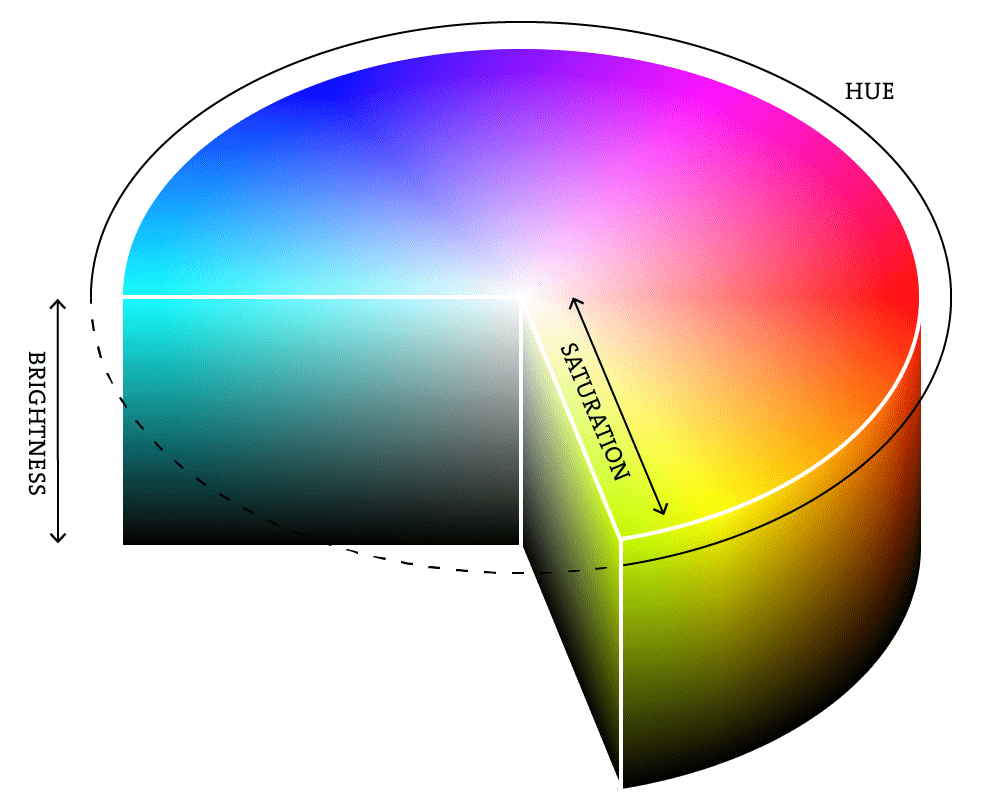
\includegraphics[width=0.6\columnwidth]{pictures/nguyen-tac-phoi-mau-18.png}
    \caption{Ba yếu tố chi phối màu sắc răng}
    \label{fig:nguyen-tac-phoi-mau}
\end{figure}

\textbf{
\section{Các yếu tố ảnh hưởng đến so màu trong nha khoa}}
\vspace{-5pt}
\subsection{Ánh sáng}
\vspace{-5pt}
\qquad Không thể so màu chính xác khi thiếu hoặc thừa ánh sáng, ánh sáng khi so màu răng phụ thuộc vào nguồn sáng và cường độ sáng khi ánh sáng chiếu đến vật thể so màu và phản xạ lại mắt người so màu.\par
\vspace{-5pt}
\quad Cường độ ánh sáng (độ sáng) ảnh hưởng đến đường kính giãn đồng tử của người so màu, ảnh hưởng đến kết quả so màu. Cường độ thích hợp để so màu trong nha khoa là vừa đủ để đồng tử giãn và ánh sáng phản xạ từ vật thể tập trung vào hố thị giác của võng mạc, từ 1000-2000 lux, được xác định bằng dụng cụ ánh sáng kế.\par
\vspace{-5pt}
\quad Hiện nay, trong nha khoa thường dùng ánh sáng lý tưởng để so màu là ánh sáng hiệu chỉnh (Color-corrected light) với cường độ sáng khoảng 1000-2000 lux và nguồn màu từ 5500-6500K.\cite{TruongDinhKhoi}

%chèn ảnh bảng nhiệt độ màu K
\begin{figure}[h]
    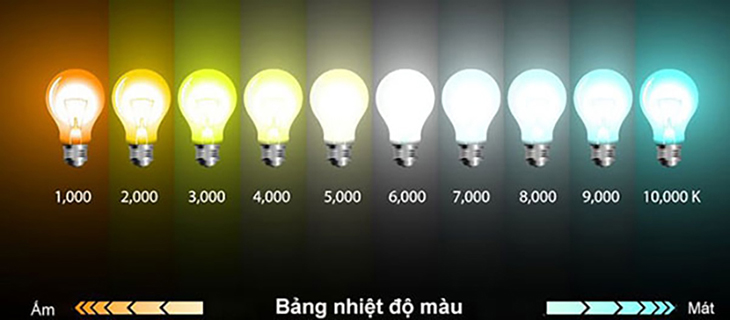
\includegraphics[width=1\columnwidth]{pictures/bảng nhiệt độ màu K.jpeg}
    \caption{Dải màu nhiệt của nguồn sáng}
    \label{fig:bảng nhiệt độ màu K}
\end{figure}

\subsection{Sự xung đột ánh sáng trong không gian so màu}
\vspace{-5pt}
\qquad Trong không gian phòng khám để so màu, nơi pha trộn giữa nhiều nguồn sáng như ánh sáng tự nhiên, ánh sáng đèn chiếu sáng, ánh sáng từ nguồn hiệu chỉnh so màu, vì vậy cần hạn chế sử dụng nhiều nguồn sáng, các nguồn sáng hỗ trợ cần có màu tương thích với màu hiệu chỉnh khi so màu hoặc màu trung tính như màu xám. Màu ánh sáng hiệu chỉnh cần thống nhất và theo chuẩn hoá hiệu chỉnh để kết quả được chính xác và tương đồng nhau. Khi màu nguồn sáng khác nhau sẽ cho ra những kết quả so màu khác nhau (hiện tượng metame so màu).\cite{TruongDinhKhoi}


%chèn ảnh màu sắc răng khác nhau 
\begin{figure}[h]
    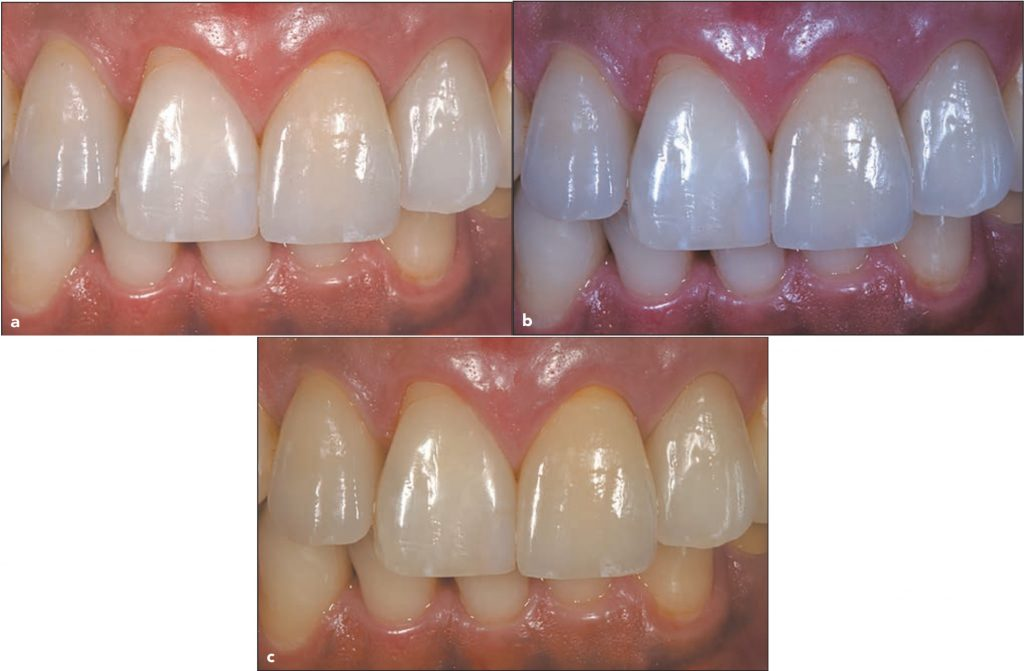
\includegraphics[width=1\columnwidth]{pictures/màu sắc răng khác nhau khi nguồn màu khác nhau.jpeg}
    \caption{Màu răng khác nhau khi nguồn màu khác nhau}
    \label{fig:màu sắc răng khác nhau khi nguồn màu khác nhau}
\end{figure}

\subsection{Hiệu ứng tương phản đồng thời trong so màu nha khoa}
\vspace{-5pt}
\qquad Tương phản đồng thời khi quan sát và so sánh màu sắc của hai hay nhiều màu cùng một lúc, khi đó mắt và não có xu hướng cân bằng và trung bình màu. Sự tương phản đồng thời ảnh hưởng bởi ba yếu tố: Cường độ sáng xung quanh (vật thể sẽ có màu tối hơn nếu vật thể xung quanh sáng hơn và ngược lại); màu của môi trường xung quanh (vật thể có xu hướng ảnh hưởng cân bằng với các màu xung quanh); độ bão hoà môi trường xung quanh (màu của vật thể có xu hướng sẫm hơn nếu môi trường ít bão hoà hơn và ngược lại).
\vspace{-5pt}
\setlength{\parskip}{-1pt}
\begin{itemize}
    \item{Tương phản đồng thời về giá trị cường độ sáng (tương phản Value)}
\end{itemize}
\vspace{-5pt}
\qquad Độ sáng của vật thể so màu bị ảnh hưởng bởi những màu nền xung quanh, màu nền tối thì vật sẽ nhìn sáng hơn và ngược lại. Mắt thích nghi với sự thay đổi màu nền từ tối sang sáng nhạy hơn so với chuyển màu nền từ sáng sang tối. Trong nha khoa, khi viền lợi bị viêm thì cổ răng sẽ sáng hơn hơn so với màu thật vì viền lợi viêm sẽ sưng và đỏ hơn so với màu lợi bình thường. Để khắc phục tương phản value thì nên chọn màu răng sáng với những bệnh nhân có tông màu sáng của răng xung quanh hoặc mô mềm xung quanh, và ngược lại.\cite{TruongDinhKhoi}

%ảnh màu sắc răng trên nền sáng tối
\begin{figure}[h]
 \centering
    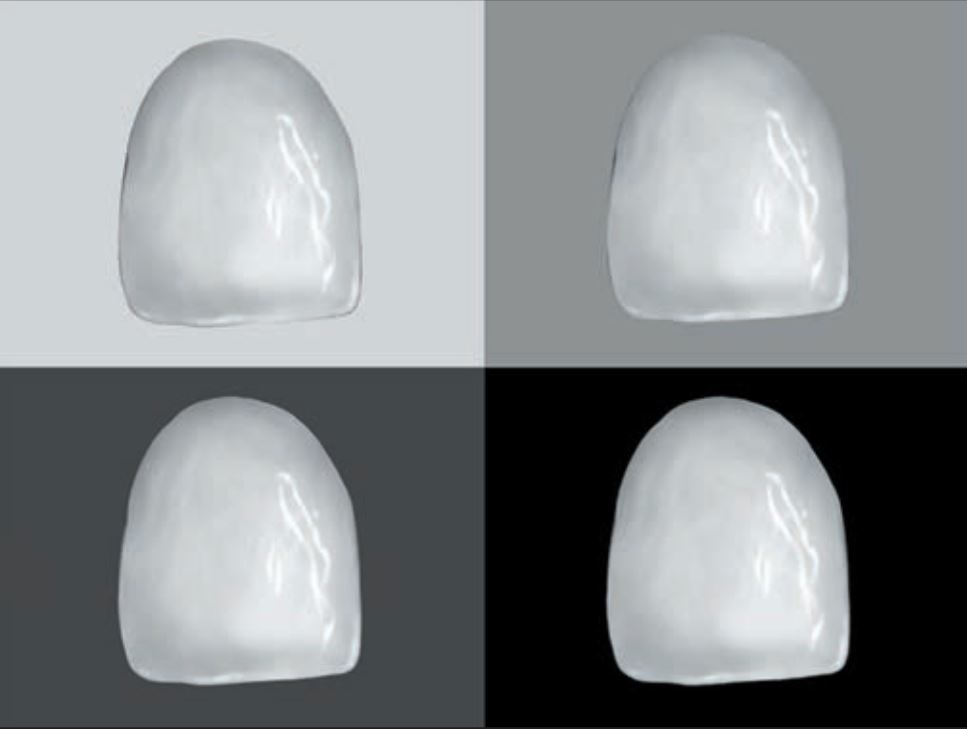
\includegraphics[width=0.8\columnwidth]{pictures/ảnh màu sắc răng trên nền sáng tối.jpeg}
    \caption{Răng sẽ sáng hơn nếu màu nền tối hơn}
    \label{fig:ảnh màu sắc răng trên nền sáng tối}
\end{figure}

\begin{itemize}
    \item{Tương phản đồng thời về màu (tương phản Hue)}
\end{itemize}
\vspace{-5pt}
\qquad Màu của vật thể có thể bị ảnh hưởng bởi màu của màu nền xung quanh. Ví dụ, răng hoặc miếng trám sẽ xanh hơn khi màu nền màu cam hoặc sẽ tím hơn nếu màu nền màu vàng. Như vậy, màu vật thể có xu hướng trung hòa với màu nền của môi trường xung quanh. Khi quan sát một màu cùng lúc với màu khác thì hue cảm nhận đầu tiên nhận được sẽ giống với màu bổ sung thứ 2, do vậy bác sĩ nên nhìn vào màu bổ sung trước khi nhìn vào màu của răng. Hầu hết màu răng đều nằm trong nhóm màu cam nên bác sĩ nên nhìn vào màu xanh dương trước khi so màu để giảm tương phản hue.\cite{TruongDinhKhoi}
\vspace{-5pt}
%chèn ảnh hue ạ


\begin{itemize}
    \item{Tương phản đồng thời về độ bão hoà (tương phản Chroma)}
\end{itemize}
\vspace{-5pt}
\qquad Độ bão hoà của vật thể sẽ lớn hơn nếu độ bão hoà của nền thấp hơn và ngược lại. Như vậy, nếu hue và chroma của vật thể càng giống với hue và chroma của màu nền thì càng khó so và phân biệt màu của vật thể đó. Trong nha khoa, không nên chọn màu nền có hue và chroma giống với hue và chroma của răng.\cite{TruongDinhKhoi}
\begin{figure}[h!]
  \centering
    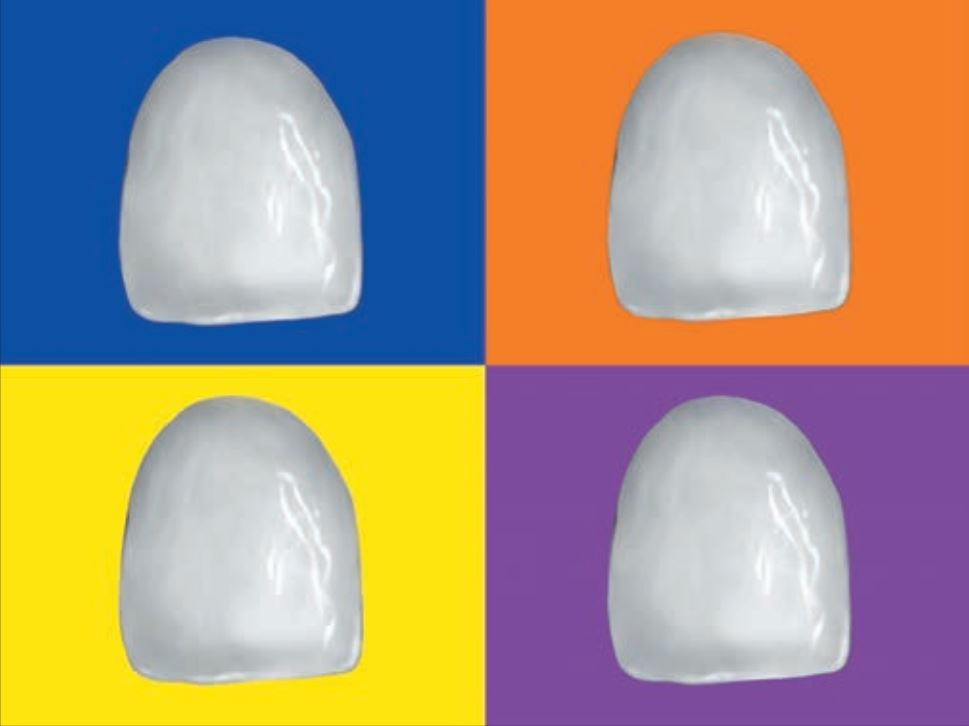
\includegraphics[width=0.6\columnwidth]{pictures/hue.jpeg}
    \caption{Răng có xu hướng trung hòa với màu nền, răng tím hơn nếu nền màu vàng, màu cam hơn nếu nền màu xanh dương, vàng hơn nếu màu nền màu tím và tím hơn nếu nền màu vàng}
    \label{fig:hue}
\end{figure}
%chèn ảnh chroma :3 lại còn có cái mông =))))) cho nó cute á, đỡ bị chán ạ
\begin{figure}[h!]
   \centering
    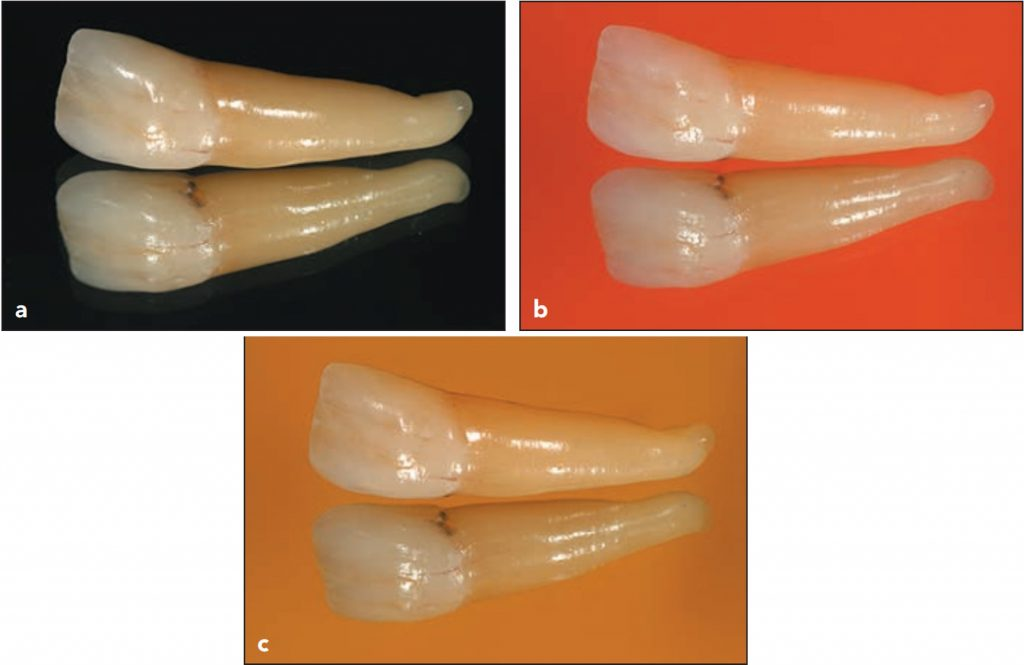
\includegraphics[width=0.7\columnwidth]{pictures/chroma.jpeg}
    \caption{a – màu răng không bị ảnh hưởng bởi chroma, b- nền màu đỏ-cam thì khó xác định màu hơn, c- nền màu vàng – cam còn khó xác định hơn nữa}
    \label{fig:chroma}
\end{figure}

\subsection{Hiệu ứng tương phản vùng khi so màu nha khoa}
\qquad Kích thước của vật thể cũng ảnh hưởng đến màu quan sát được, kích thước lớn hơn thì cảm nhận màu sáng hơn so với vật thể có kích thước nhỏ. Trong thực hành nha khoa, nếu răng có kích thước lớn thì màu chọn thường sẽ nên tối hơn so với mức bình thường vì cảm nhận màu của người quan sát sẽ thấy sáng hơn và ngược lại. Nếu răng hoặc miếng trám lớn thì nên tăng độ hue và ngược lại.\cite{TruongDinhKhoi}

\subsection{Hiệu ứng không gian khi so màu nha khoa}
\qquad Vật thể càng gần mắt người quan sát thì càng sáng hơn và lớn hơn, và ngược lại, càng ở xa thì càng nhỏ và tối hơn. Trong nha khoa, răng phía trước có xu hướng sáng hơn răng phía sau, răng chen chúc thì phía trước sáng hơn răng chen chúc phía sau. Vì vậy, bác sĩ nên giữ đồng nhất khoảng cách từ mắt đến răng so màu, và có kế hoạch bù trừ màu với răng thụt vào thì màu nên cho sáng hơn so với răng nhô ra so với cung hàm.\cite{TruongDinhKhoi}

%chèn ảnh không gian so màu
\begin{figure}[h]
\centering
    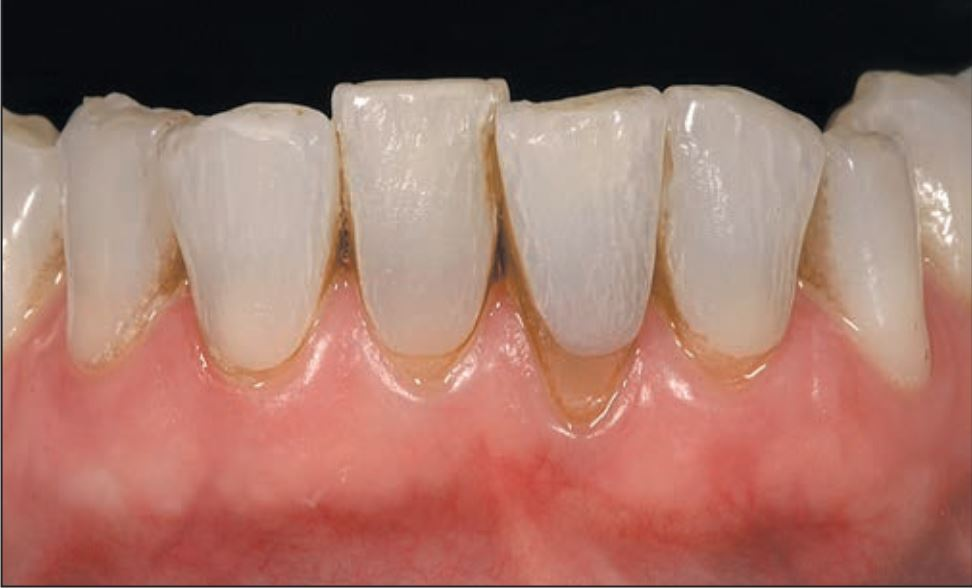
\includegraphics[width=0.7\columnwidth]{pictures/không gian so màu.jpeg}
    \caption{Răng 41 có vẻ tối hơn so với răng 31 do hiệu ứng không gian}
    \label{fig:không gian so màu}
\end{figure}

\subsection{Hiệu ứng tương phản dư ảnh khi so màu nha khoa}
\qquad Xảy ra khi vừa quan sát một màu trong một khoảng thời gian đủ lâu sau đó ngay lập tức quan sát một màu khác, màu quan sát trước đó sẽ dư ảnh và ảnh hưởng thành màu tương phản khi quan sát trên nền trắng. Có hai loại dư ảnh: Dư ảnh âm bản (tương phản màu thực) và dư ảnh dương bản (trở lại màu thực).\cite{TruongDinhKhoi}


\subsection{Nhận thức màu kém}
\qquad Những người có khiếm khuyết trong nhận thức màu sắc thì khó khăn trong việc xác định màu của vật thể, có thể kém nhận thức một hoặc nhiều màu, mức độ có thể từ nhẹ đến mức hoàn toàn không nhận thức màu sắc.\cite{TruongDinhKhoi}\par

%ảnh mù màu
\begin{figure}[h]
\centering
    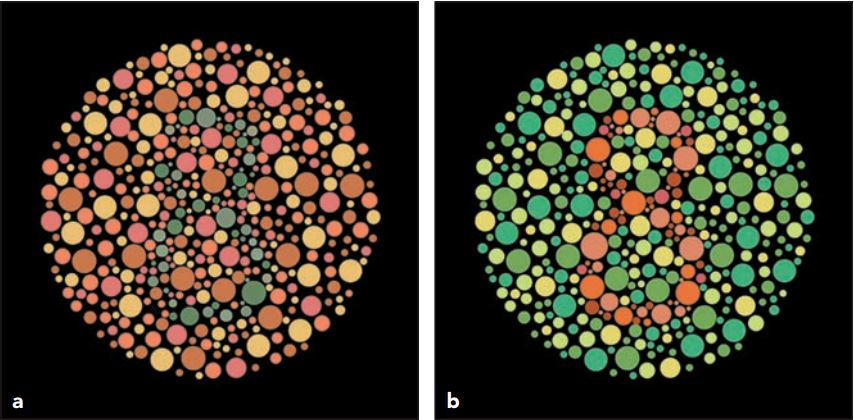
\includegraphics[width=0.8\columnwidth]{pictures/mù màu.jpeg}
    \caption{Bảng test màu a): test độ nhạy với màu xanh lá và màu vàng để phát hiện số 8; b): test ngược, số 8 dễ nhận thấy hơn với màu tím- đỏ}
    \label{fig:mù màu}
\end{figure}


\quad Khi bị khiếm khuyết về màu thì cảm nhận hue bị sai lệch so với chuẩn của người bình thường, giảm khả năng phân biệt màu, độ bão hoà hoặc độ sáng tối của màu.\cite{TruongDinhKhoi}

%ảnh mắt??
\begin{figure}[h!]
\centering
    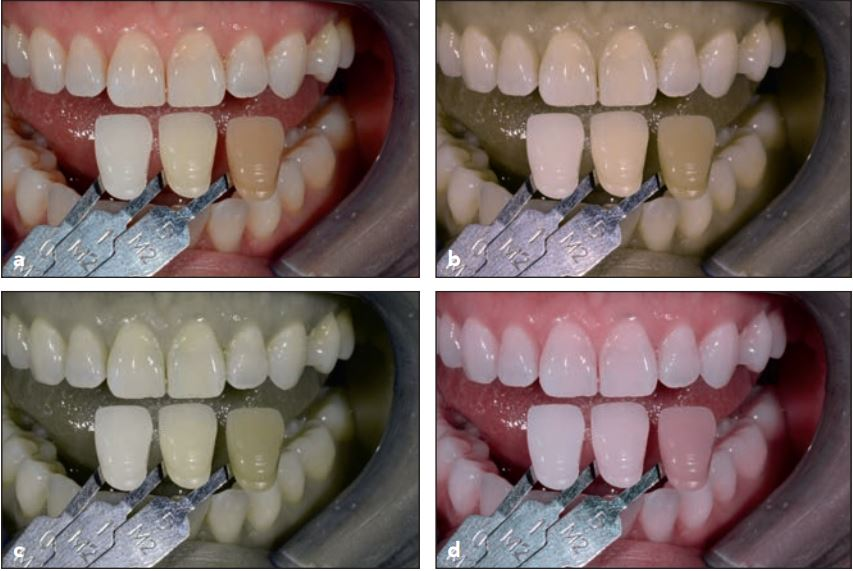
\includegraphics[width=0.8\columnwidth]{pictures/mắt.jpeg}
    \caption{a): Hình ảnh so màu của người bình thường, b): so màu của người mù màu đỏ, c): so màu của người mù màu xanh lá, d): so màu của người mù màu xanh dương}
    \label{fig:mắt}
\end{figure}

\subsection{Tuổi}
\qquad Tuổi ảnh hưởng đến kết quả so màu khi thuỷ tinh thể và giác mạc sẽ đục dần theo tuổi, có xu hướng nghiêng dần về màu vàng-nâu theo tuổi nên khó phân biệt hơn giữa mùa trắng và màu vàng. Quá trình giảm nhạy cảm màu sau tuổi 30 và rõ ràng khi bước sang tuổi 60, nhiều người ở tuổi 60 gặp khó khăn với màu tím và màu xanh dương.\cite{TruongDinhKhoi}

\subsection{Sức khoẻ thể chất của người quan sát}
\qquad Sự mệt mỏi có thể ảnh hưởng đến quá trình so màu, mệt mỏi ở mắt và toàn thân có sự ảnh hưởng khác nhau, khi mắt mệt mỏi thì người so màu có xu hướng thích nghi với màu sắc. Sự thích nghi phần lớn là điều chỉnh độ nhạy với màu sắc của các thụ thể nhận cảm. Sự nhận cảm của tế bào nón chia thành ba cặp màu đối lặp: xanh dương-vàng, đỏ-xanh lá, đen-trắng. Sự kích thích một màu bất kỳ sẽ gây ức chế các cặp còn lại, như vậy khi mắt mệt mỏi thì không thể đưa ra phán đoán chính xác về màu sắc, đặc biệt sau khi bị kích thích bởi một màu quá nhiều. Sự mệt mỏi toàn thân cũng gậy ra những sai lệch trong nhận thức màu sắc.\cite{TruongDinhKhoi}

 \subsection{Sự thích nghi ánh sáng và bóng tối của người quan sát}
 \qquad Sự thích nghi ánh sáng và bóng tối là khả năng ít bị nhạy cảm trước kích thích của màu sắc khi thay đổi về các đặc tính của màu như giá trị màu, độ sáng và độ bão hòa của màu. Có ba sự thích nghi ảnh hưởng đến nhận thức màu là thích nghi ánh sáng, bóng tối và màu sắc. Thích nghi với ánh sáng là sự giảm độ nhạy cảm của thị giác khi mức độ chiếu sáng tổng thể tăng lên. Ví dụ, khi bước vào căn phòng chiếu sáng tốt ngay sau khi rời khỏi căn phòng tối, thích nghi bằng cách ít nhạy cảm hơn, thường mất khoảng 5 phút để thiết lập hoàn toàn sự thích nghi này. Sự thích nghi bóng tối là quá trình ngược lại với thích nghi ánh sáng, trở nên nhạy cảm hơn với ánh sáng, thường mất khoảng 30 phút để thiết lập hoàn toàn. Sự thích nghi màu sắc là ít nhạy cảm khi có sự thay đổi màu sắc liên tục.\cite{TruongDinhKhoi}

 \subsection{Dinh dưỡng}
 \qquad Chế độ dinh dưỡng đóng một vai trò quan trọng đối với người so màu nói riêng và con người nói chung, trong đó vitamin A có vai trò ảnh hưởng trực tiếp đến thị lực, lượng vitamin A cần thiết mỗi ngày trong khoảng từ 900-3000 microgram (mcg)/ngày.\cite{TruongDinhKhoi}

\subsection{Cảm xúc}
\qquad Trạng thái cảm xúc của con người có ảnh hưởng đến quá trình xác định và đánh giá màu sắc, ngoài cảm xúc hoặc tâm trạng thì sở thích về màu sắc cũng có liên quan đến chọn lựa màu sắc. Do vậy, trong thực hành nha khoa, trước khi so màu, người quan sát cần thư giãn và mời thêm cộng sự so màu cùng để đưa ra những kết luận chính xác hơn.\cite{TruongDinhKhoi}

\subsection{Rối loạn nhận thức màu do thuốc}
\qquad Thuốc có thể thay đổi nhận thức về màu sắc do làm thay đổi về chất dẫn truyền thần kinh, thay đổi độ nhạy về màu do liên quan đến chuỗi phản ứng hóa học của các thụ thể võng mạc. Ví dụ, thuốc nhóm phosphodiesterase như sildenafil làm sai lệch nhận thức màu xanh dương. Thuốc điều hòa nhịp tim như amiodarone hoặc thuốc điều trị bệnh lao như ethambutol gây rối loạn màu sắc.\cite{TruongDinhKhoi}

\subsection{Sự khác biệt giữa hai mắt người quan sát}
\qquad Màu sắc được sự phối hợp và thống nhất giữa hai mắt khi cùng nhìn về vật thể, sự chênh lệch thị lực giữa hai mắt có thể gây ra những sai lệch khi so màu. Khi đặt hai vật thể giống nhau cạnh nhau thì thấy khác nhau về màu sắc, điều đó chứng tỏ hai mắt không tương đồng về cảm nhận màu sắc.\cite{TruongDinhKhoi} 

\subsection{Các đặc tính quang học của men và ngà}
\par 
\qquad Các thuộc tính của men/ngà ảnh hưởng đến nhận thức màu sắc của răng bao gồm độ trong/mờ (translucency/opacity), độ huỳnh quang (fluorescence), độ trắng đục (opalescence) và độ sáng bóng (gloss). Độ trong/mờ tuyệt đối gọi là transparency, cho ánh ánh sáng truyền qua hoàn toàn, không xảy ra hiện tượng phản xạ hay hấp thụ ánh sáng, tương ứng độ đục bằng 0. \cite{TruongDinhKhoi}

\textbf{
\section{Bảng so màu Vita 3D Master}}
\quad Bảng so màu Vita 3D Master được ký hiệu theo thứ tự số - chữ cái - số (ví dụ 3M2), trong đó thể hiện theo thứ tự giá trị của hue, value và chroma.\cite{TruongDinhKhoi} Theo thứ tự value, chia thành sáu nhóm có giá trị value giảm dần từ nhóm 0 đến nhóm 5:\par
\quad \textit{Nhóm 0:} Nhóm có value cao nhất, chỉ có một hue ký hiệu M (màu trung tính) có 3 cây 0M1, 0M2, 0M3 theo thứ tự tăng dần chroma từ nhạt đến sẫm màu hơn 0M1<0M2<0M3.\par
\quad \textit{Nhóm 1:} 2 cây 1M1 và 1M2, có cùng hue màu trung tính ký hiệu M, có thứ tự tăng dần chroma 1M1<1M2.\par
\quad \textit{Nhóm 2, 3 và 4:} Có 7 cây, chia thành 3 phân nhóm nhỏ theo thứ tự thay đổi hue gồm: nhóm L (left) - màu vàng, nhóm M (medium) - màu trung tính, nhóm R (right) - màu đỏ. Trong nhóm L, độ chroma tăng dần 2L1<2L2; 3L1<3L2; 4L1<4L2. Trong nhóm M, độ chroma tăng dần 2M1<2M2<2M3; 3M1<3M2<3M3; 4M1<4M2<4M3. Trong nhóm R, độ chroma tăng dần 2R1<2R2; 3R1<3R2; 4R1<4R2.\par
\quad \textit{Nhóm 5:} Có 3 cây, nhóm có value thấp nhất, chỉ có một hue ký hiệu M tương tự nhóm 0 (màu trung tính), 3 cây gồm 5M1, 5M2, 5M3 theo thứ tự tăng dần chroma 5M1<5M2<5M3.\par

%chèn ảnh bảng so màu vào đây nháaa
\begin{figure}[h]
\centering
    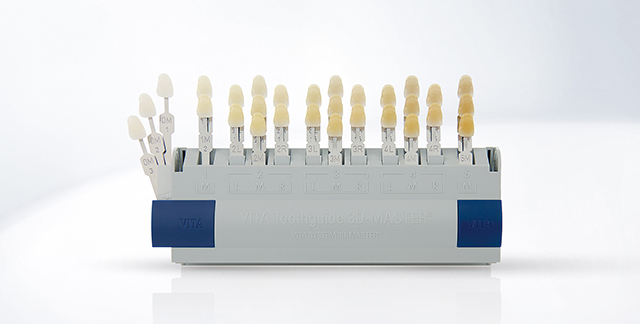
\includegraphics[width=0.7\columnwidth]{pictures/anh-vita-3d.jpeg}
    \caption{Bảng so màu Vita 3D Master}
    \label{fig:anh-vita-3d}
\end{figure}

\quad \textbf{Các bước so màu sử dụng bảng màu Vita:}\par
\quad \textit{Bước 1: }Chọn value, chọn một trong sáu nhóm sao cho độ sáng của răng giống nhất với độ sáng của các cây loại M trong bảng so màu từ nhóm value đã chọn được.\par
\quad \textit{Bước 2:} Chọn chroma, từ các cây loại M đã chọn xác định cây có chroma gần giống nhất với răng được so màu.\par
\quad \textit{Bước 3:} Chọn hue, từ các cây có cùng value và chroma, so sánh với các cây loại L và R có cùng value và chroma với cây loại M vừa chọn, từ đó chọn ra cây có hue gần giống nhất với răng so màu, viết ký hiệu màu chọn theo quy ước của bảng so màu.
\vspace{5pt}
\textbf{
\section{Các nguyên tắc khi so màu}}
\quad Trước khi so màu cần đảm bảo đủ tiêu chuẩn về nguồn sáng, lý tưởng nhất dưới ánh sáng tự nhiên và đủ tiêu chuẩn kỹ thuật trên. Loại bỏ màu sắc gây nhiễu xung quanh răng so màu, tránh sử dụng màu sắc khác gây nhiễu loạn và mỏi mắt trước và trong khi so màu.\cite{TruongDinhKhoi}\par

\quad Vị trí đặt bảng so màu phụ thuộc vào phương pháp so màu và mục đích so màu, so màu pha macro thì đặt bảng so màu, sau đó chọn các cây tiếp tục cho pha sau như pha mini và pha micro.\par

\quad Có thể đặt giữa răng hàm trên và hàm dưới hoặc kế bên ngang mức rìa cắn răng cần so màu, tránh đặt chồng lên phía trước hoặc phía sau răng cần so màu\par

%ảnh nguyên tắc so màu 
\begin{figure}  [h]
    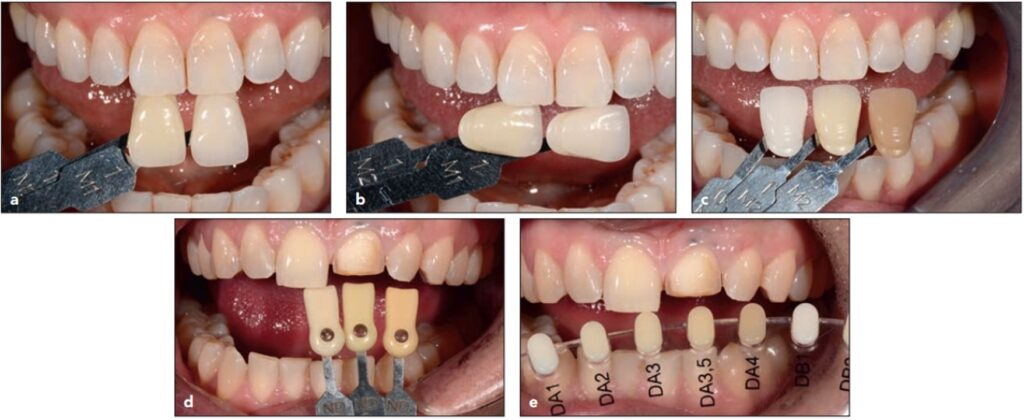
\includegraphics[width=1\columnwidth]{pictures/nguyên tắc so màu.jpeg}
    \caption{a): đặt cổ - rìa cắn, b): đặt nằm ngang, c): đặt đối đầu, d và e): so màu cùi răng}
    \label{fig:nguyên tắc so màu}
    \end{figure}
    
\quad Phương pháp so màu theo mô hình ba pha macro - mini - micro, bắt đầu bằng pha macro bằng cách sử dụng toàn bộ bảng so màu, chọn và đặt sang một bên các màu được lựa chọn để dùng cho pha sau, loại bỏ các màu không phù hợp. Ở pha mini, các cây được lựa chọn thì chọn tiếp sao cho phù hợp về màu của cổ, thân và rìa cắn gần nhất với răng cần so màu. Ở pha micro thì so sánh chi tiết về hue, value và chroma. Không đặt rìa cắn hướng về phía kim loại của bảng so màu.\par
\quad Nên so màu răng cả cùi răng và so màu từng phần của răng thành ba phần rìa cắn, thân và cổ răng. Kết quả so màu cần ghi ký hiệu màu dưới dạng “ngôn ngữ màu (color language)” theo từng loại bảng so màu của nhà sản xuất nhằm thống nhất màu giữa bác sĩ và labo răng.\par
\vspace{-5pt}
\textbf{
\section{Các phương pháp so màu}}
\quad Hiện nay có nhiều phương pháp đánh giá màu răng như sử dụng bảng so màu băng giấy, sứ có màu hoặc nhựa acrylic, sử dụng quang phổ kế, sắc kế và kỹ thuật phân tích hình ảnh.\cite{NguyenThiChau}\par
\quad Việc xác định màu bằng cách so màu răng với màu răng mẫu trên bảng so màu là ứng dụng phổ biến nhất trong nha khoa. Răng và bảng so màu được quan sát cùng lúc dưới điều kiện ánh sáng như nhau. Ánh sáng bên ngoài, kinh nghiệm, tuổi, sự mỏi mắt và vấn đề sinh lý (mù màu) có thể dẫn tới mâu thuẫn và sai lệch. Mặt khác tiêu chuẩn hóa thuộc tính màu sắc được đánh giá bằng thị giác bị giới hạn. Theo Joiner (2004), màu cơ bản của một răng được xác định ở một phần ba giữa răng bởi vì dải màu thay đổi từ rìa cắn tới viền lợi và quan sát viên phải tập trung vào vùng này. \par
\quad Xác định màu bằng quang phổ kế: Theo Andjelkovic (2010) và Lenhmann (2010) là đo một độ dài bước sóng tại thời điểm từ khi truyền ánh sáng của một đối tượng và được sử dụng để đo quang phổ hữu hình của những răng đã nhổ và răng sống. Theo Corciolani (2007), sử dụng quang phổ kế đo màu sắc là chính xác nhất.\cite{NguyenThiChau}	\par	
\quad Sắc kế có bộ lọc màu xấp xỉ chức năng quang phổ của mắt quan sát viên đạt tiêu chuẩn và được đo màu trong 3 nhóm màu cơ bản trong hệ thống màu CIE L, a*, b*. Phép đo bằng sắc kế đã được so sánh với sự ghi quang phổ kế là đáng tin cậy và chính xác để đo lường màu sắc.\cite{NguyenThiChau}\par
\vspace{-5pt}
\textbf{
\section{Chỉ số nhu cầu điều trị làm trắng răng}}
\quad Khi xây dựng chỉ số nhu cầu điều trị tẩy trắng răng, điều quan trọng là phải xem xét nhu cầu điều trị dựa trên nhiều tình huống bao gồm các vấn đề bẩm sinh như khuyết tật di truyền của răng hoặc khuyết tật bẩm sinh như mảng trắng hoặc nâu.\cite{LindaGreenwall2019}\par
\quad Theo Whitening Group, giới hạn được thiết lập bởi các quy định hiện hành gây khó khăn cho việc điều trị bệnh nhân một cách dễ dàng và tiết kiệm chi phí; tuy nhiên, những người có các chỉ định sau nên được ưu tiên\cite{LindaGreenwall2019}:\par
\begin{enumerate}
    \setlength{\itemsep}{0pt}
    \item Sự đổi màu nghiêm trọng và trung bình.
    \item Điều kiện tráng men.
    \item Đốm trắng và vết trắng nhỏ.
    \item Nhuộm màu nâu, cam và vàng.
    \item Khiếm khuyết về mặt thẩm mỹ.
    \item Răng cửa mọc lệch lạc.
    \item Thiểu sản răng cửa hàm.
    \item Chấn thương.
    \item Yếu tố di truyền, ví dụ: sự tạo men răng bất toàn.
    \item Có răng trước bị đổi màu không còn sức sống.
\end{enumerate}
\par
\quad Các cân nhắc khác nhau được đưa ra khi đánh giá các chỉ định cho nhu cầu điều trị\cite{LindaGreenwall2019}:\par
\begin{itemize}
\setlength{\itemsep}{0pt}
    \item Sắc thái của sự đổi màu (ví dụ: các sắc thái rất đậm—A4, C4, B4): sự đổi màu như vậy (dấu hiệu 1) được chia thành nghiêm trọng, trung bình và nhẹ. Điều trị tẩy trắng nên được thực hiện nếu loại đổi màu có thể được xếp vào loại nghiêm trọng hoặc trung bình, trẻ nhận thức được sự đổi màu và sự đổi màu có ảnh hưởng đến cuộc sống của trẻ.
    \item Tính chất và mức độ biến màu.
    \item Sự đổi màu có lan rộng trên răng hay không hoặc có lốm đốm trên răng hay không.
    \item Răng có màu sắc bình thường nhưng có vết trắng, lốm đốm hoặc vệt trắng.
    \item Sự hiện diện của sự đổi màu nâu trên bề mặt môi trong của răng, có thể do chấn thương (chảy máu vào răng trước đó) hoặc dấu hiệu nhiễm fluorosis. Đôi khi không rõ nguyên nhân. \item Thông thường, phần đổi màu nâu sẽ được loại bỏ đầu tiên khi quá trình điều trị làm trắng bắt đầu và là phần làm sáng nhanh nhất. Đôi khi có thể mất nhiều thời gian hơn để điều trị làm trắng loại bỏ hoàn toàn đốm nâu. Nó có thể mờ dần thành một vết màu vàng nhạt. Khi màu nền được làm sáng, dấu hiệu sẽ ít được chú ý hơn. Các vết đổi màu nâu có thể được loại bỏ khoảng 80\% thời gian (Haywood 2006). Chỉ có một số vùng màu nâu cần xử lý lại sau 1-3 năm (Haywood 2006).
    \item Xuất hiện các mảng trắng trên răng cửa và răng hàm. Ngày càng có nhiều đốm trắng trên răng. Các đốm và mảng trắng có thể lan rộng trên các răng trước cũng như các răng hàm đầu tiên. Nếu có tình trạng này thì chỉ định can thiệp phục hồi răng hàm sớm cũng như điều trị tẩy trắng răng để giảm ảnh hưởng của các vết trắng trên bề mặt môi trong của răng.
    \item Ảnh hưởng của sự đổi màu đối với trẻ.
    \item Sự đổi màu có dễ dàng được tẩy trắng hay có thể yêu cầu nhiều lựa chọn xử lý như tẩy trắng, xử lý bề mặt men răng như xử lý Sylc, phun cát, mài mòn siêu nhỏ (12–26 micron men được loại bỏ sau 5 giây sử dụng; Haywood 2006), hoặc xâm nhập nhựa.
    \item Liệu có sự đổi màu răng đơn lẻ chẳng hạn như răng chết do chấn thương hay không.
    \item Có nhiều vết đổi màu trên toàn bộ răng hay không. Bệnh nhân với các điều kiện được đề cập bởi Nhóm làm việc nên được điều trị với kế hoạch điều trị thích hợp theo chẩn đoán.
\end{itemize}

\quad \textbf{Chỉ số về nhu cầu điều trị tẩy trắng răng cho bệnh nhân dưới 18 tuổi:}\cite{LindaGreenwall2019}\par
\textbf{Loại 1 - Cao}
\begin{enumerate}
\setlength{\itemsep}{0pt}
    \item Sự đổi màu: nghiêm trọng
    \item Vị trí vết: phân bố nhiều đậm nhạt đồng đều
    \item Ảnh hưởng đến trẻ em: nghiêm trọng
    \item Nhu cầu làm trắng: cao
\end{enumerate}

\textbf{Loại 2 - Trung bình}
\begin{enumerate}
\setlength{\itemsep}{0pt}
    \item Sự đổi màu: vừa phải
    \item Vị trí: phân bố đều
    \item Ảnh hưởng đến đứa trẻ: có ảnh hưởng đến đứa trẻ
    \item Nhu cầu làm trắng: vừa phải
\end{enumerate}

\textbf{Loại 3 — Mong muốn}
\begin{enumerate}
\setlength{\itemsep}{0pt}
    \item Sự đổi màu: nhẹ
    \item Vị trí: ít răng trước
    \item Tác động đến trẻ em: một số tác động
    \item Nhu cầu làm trắng: mong muốn; điều này sẽ dễ dàng làm giảm bớt các vấn đề đổi màu
\end{enumerate}

\textbf{Loại 4 — Khuyến cáo}
\begin{enumerate}
\setlength{\itemsep}{0pt}
    \item Sự đổi màu: các khu vực bị đổi màu bị cô lập
    \item Vị trí: phân bố ngẫu nhiên trên răng
    \item Ảnh hưởng đến trẻ em: vừa phải
    \item Nhu cầu làm trắng: khuyến cáo
\end{enumerate}

\textbf{Loại 5 — Có thể}
\begin{enumerate}
\setlength{\itemsep}{0pt}
    \item Sự đổi màu: đổi màu nhẹ hoặc đốm trắng
    \item Vị trí: ít răng hoặc một răng
    \item Ảnh hưởng đến trẻ em: không ảnh hưởng đến trẻ em
    \item Nhu cầu làm trắng: có thể thực hiện được; có thể được mong muốn, nhưng có thể đợi cho đến khi đứa trẻ trên 18 tuổi.
\end{enumerate}
\vspace{-5pt}
\textbf{
\section{Các nghiên cứu trên thế giới và Việt Nam về màu sắc răng và nhu cầu làm trắng răng}}
\subsection{Trên thế giới}
\qquad Trong bài viết “Dental Whitening: Self-Referred Needs versus Professional Indication” của Renata Pedrosa Guimarães (2021) đã có những thảo luận như sau:\par
\quad Về các câu hỏi liên quan đến tẩy trắng răng, đáng chú ý là: chỉ có 15,5\% trả lời khẳng định là đã thực hiện tẩy trắng răng rồi. Trong số này, 6,9\% đã trải qua tẩy trắng răng bằng cách sử dụng kỹ thuật tại phòng khám, 5,2\% đã trải qua quá trình làm trắng có giám sát và một cá nhân đã sử dụng thuốc không kê đơn sọc trắng. Đa số (63,8\%) cho biết cần tẩy trắng răng trong câu hỏi về ai hoặc cái gì đưa ra các tiêu chuẩn liên quan đến màu sắc lý tưởng của nụ cười, hơn một nửa (56,9\%) đã trả lời rằng đó là “Phương tiện truyền thông”, tiếp theo là 19,0\% là “Lòng tự trọng” và 10,3\% cho rằng đó là “Xã hội”.\cite{Renata2021} \par
\quad Sự so sánh giữa tần suất học sinh đã tẩy trắng răng theo độ tuổi và giới tính, nơi có thể quan sát thấy tỷ lệ đã trải qua răng nhóm tuổi từ 20 đến 46 làm trắng cao hơn so với nhóm tuổi từ 18 đến 19 (22,2\% so với 9,7\%) và điều này tỷ lệ phần trăm chỉ cao hơn 1,3\% ở nữ (16,1\% so với 14,8\%), tuy nhiên đối với biên độ sai số của thống kê kiểm tra (5\%) không có mối liên hệ đáng kể nào giữa câu hỏi với bất kỳ biến nào trong hai biến được phân tích (p>0,05).\cite{Renata2021}\par
\quad Trong nghiên cứu về câu hỏi "Bạn có nghĩ rằng bạn cần phải làm trắng răng?" Tỷ lệ trả lời khẳng định là: nữ cao hơn nhiều so với nam (p=0,001). Các câu trả lời là khẳng định đối với hầu hết sinh viên trong tất cả các khóa học, ngoại trừ những người trong các khóa học y khoa, với sự nhấn mạnh về dinh dưỡng học sinh (70,0\%) và học thể dục (63,6\%). Sự liên kết giữa câu hỏi là
kiểm chứng cho cả hai biến (p<0,05). Tám (88,9\%) trong số chín cá thể được chụp ảnh có màu tối hơn trên thang đo so với màu thực tế được hiển thị bởi máy đo quang phổ kỹ thuật số. Chỉ dành cho một trong số họ (11,1\%), các giá trị này trùng nhau.\cite{Renata2021}\par
\quad Kết quả của 180 đánh giá được thực hiện bởi 20 nha sĩ ở chín cá nhân ai nói cần tẩy trắng, tùy chuyên ngành, thời gian tốt nghiệp và giảng dạy cơ sở giáo viên đã tham gia khóa học. Từ bảng này, có thể nhấn mạnh rằng: hơn một nửa (53,9\%) câu trả lời là tẩy trắng răng; có một mối liên quan đáng kể giữa chỉ định của làm trắng với chuyên ngành và thời gian kể từ khi ra trường. Tỷ lệ các dấu hiệu tích cực cao hơn trong số bác sỹ thuộc các chuyên khoa: Răng Hàm Mặt, Răng Hàm Mặt + Chỉnh Nha và Răng Hàm Mặt + Cấy Ghép Implant, và thấp hơn giữa các chuyên khoa Răng Hàm Mặt + Nội Nha, Nội Nha, Nhi Khoa và Nha Chu. Cao nhất phần trăm phản hồi có chỉ định tẩy trắng xảy ra ở những người có hơn 20 năm tốt nghiệp (65,3\%) và thấp nhất là nhóm từ 10 đến 19 tuổi (35,6\%).\cite{Renata2021}\par
\quad Hiện nay, các chuyên gia và bệnh nhân chia sẻ lý tưởng thẩm mỹ liên quan trực tiếp đến răng nhẹ. Các nhận thức về những gì là thẩm mỹ hoặc không thẩm mỹ, liên quan đến màu sắc của răng, thay đổi tùy thuộc vào bối cảnh của hiệu suất của mỗi người, bệnh nhân và các chuyên gia. Ý kiến về màu sắc của răng có một cực kỳ tính chất chủ quan và rất khác nhau giữa chuyên gia này và chuyên gia khác. Đa số bệnh nhân tự nhận thấy màu răng của họ tối hơn so với thực tế. Bệnh nhân nữ thường mong muốn có hàm răng sáng màu hơn.\cite{Renata2021}\par
\quad Cuối cùng, phương tiện truyền thông có vai trò quyết định trong việc xác định tiêu chuẩn thẩm mỹ của nụ cười.\par
\subsection{Ở Việt Nam}
\qquad Trong “Nghiên cứu hiệu quả điều trị tẩy trắng răng sống Tetracycline" của Nguyễn Thị Châu (2013) cho thấy phân bố màu sắc nhóm răng theo phổ màu Munsell: Điểm màu Vita V, độ bão hòa màu C: Cao nhất là răng nanh và thấp nhất là răng hàm nhỏ, sự khác biệt có ý nghĩa thống kê. Tông màu h: Răng nanh thấp nhất và răng hàm nhỏ là cao nhất, sự khác biệt có ý nghĩa thống kê. \par
\quad Bảng Vita cổ điển chia làm 4 nhóm màu: Nhóm A đặc trưng cho màu vàng đỏ hoặc nâu đỏ, nhóm B đặc trưng cho màu vàng, nhóm C đặc trưng cho màu xám, nhóm D đặc trưng cho màu vàng ánh đỏ theo thang điểm độ sáng tối. Màu sắc ở răng cửa (tương ứng B4) có màu vàng nâu xám nhẹ. Răng nanh (tương ứng C4 - A4) có màu vàng xám đỏ. Răng hàm nhỏ tương ứng B3 - A3.5 có màu vàng cam đỏ. Theo tông màu h xác định màu sắc trên tọa độ cực răng nanh (75,9) tương ứng màu vàng xám đỏ, răng cửa (79,4) tương ứng vàng đỏ và răng hàm nhỏ (81,7) tương ứng vàng cam, cũng tương đồng với điểm màu Vita\cite{NguyenThiChau}. \par
\quad Như vậy, màu sắc răng không đồng nhất giữa nhóm răng cửa, nanh và răng hàm nhỏ, trong đó nhóm răng phía trước màu đậm hơn so với răng phía sau, sự khác biệt có ý nghĩa thống kê. Điểm màu Vita của răng hàm nhỏ là thấp nhất, sau đó đến răng cửa, cuối cùng là răng nanh. Ngoài ra độ bão hòa màu của răng nanh là cao nhất, thấp nhất là răng hàm nhỏ.\cite{NguyenThiChau}\par



\chapter{ĐỐI TƯỢNG VÀ PHƯƠNG PHÁP NGHIÊN CỨU}

\textbf{
\section{Địa điểm và thời gian nghiên cứu}}
\qquad Địa điểm: Trường Đại học Y Dược - Đại học Quốc gia Hà Nội\par
\quad Thời gian nghiên cứu: Tháng 3 - tháng 5 năm 2023

\textbf{
\section{Đối tượng nghiên cứu}}
\subsection{Tiêu chuẩn lựa chọn đối tượng nghiên cứu:}
\qquad Sinh viên trong độ tuổi từ 18 – 25.\par
\quad Hàm răng tự nhiên, chưa được thực hiện các điều trị nha khoa trước đó như tẩy trắng răng, hàn răng hay hoặc răng giả, nắn chỉnh răng ....\par
\quad Có sức khỏe răng miệng tốt, không viêm lợi, không có cao răng mảng bám, không có  bệnh lý nội sinh và ngoại sinh ảnh hưởng đến màu sắc của răng.\par

\subsection{Tiêu chuẩn loại trừ:}
\begin{enumerate}
\setlength{\itemsep}{0pt}
    \item Người có vấn đề sức khỏe răng miệng nghiêm trọng: bệnh lý nha khoa nặng, viêm nhiễm hoặc sâu răng không điều trị.
    \item Đang được điều trị nha khoa liên quan đến màu sắc răng, chẳng hạn như tẩy trắng răng hoặc làm răng giả
    \item Những người có các yếu tố khác ảnh hưởng đến màu sắc răng, như hút thuốc lá, sử dụng các loại thức ăn, nước uống hoặc các biện pháp làm nhuộm màu răng như: cà phê, trà,...
    \item Bệnh nhân có tiền sử hoặc đang bị chấn thương răng dẫn đến thay đổi màu sắc răng.
    \item Không đồng thuận tham gia nghiên cứu hoặc không đáp ứng đầy đủ yêu cầu nghiên cứu, chẳng hạn như không hoàn thành câu hỏi khảo sát, không thực hiện các quy trình đo lường, hoặc không tuân thủ theo quy định và hướng dẫn của nghiên cứu.
\end{enumerate}
\vspace{-5pt}
\textbf{
\section{Phương pháp nghiên cứu}}
\quad Thiết kế nghiên cứu mô tả cắt ngang
\vspace{5pt}
\textbf{
\section{Phương pháp chọn mẫu}}
\quad Áp dụng công thức tính cỡ mẫu cho ước lượng một tỷ lệ:\par

\begin{equation*}
    \Large n = \mathrm{Z}_{1-\alpha/2}^{2}\frac{p(1-p)}{d^{2}}
\end{equation*}\par
%chèn công thức
\quad Trong đó:

\begin{itemize}[label={}, itemsep=-4pt]
    \item \textbf{n:} cỡ mẫu nghiên cứu cần có
    \item \textbf{p:} tỷ lệ răng có màu sáng theo Nguyễn Thị Châu (2013)\cite{NguyenThiChau} là 85\%
    \item \textbf{d:} khoảng sai lệch mong muốn tức tỷ lệ tuyệt đối được chúng tôi quy ước bằng 0,09
    \item \textbf{$\alpha$:} mức ý nghĩa thống kê được chúng tôi quy ước bằng 0.01 ứng với độ tin cậy 95\%  
    \item \textbf{$z^{2}_{1-\alpha/2}$:} giá trị Z tương ứng thu được bằng 1,96.
\end{itemize}

\par
\quad Thay vào công thức, có 
$n=1.96^{2}\times 0.85\times (1-0.85):0.09^{2}\approx 64$
\par  
\quad Cỡ mẫu tối thiểu cần cho điều tra nghiên cứu là 64 sinh viên, chúng tôi lấy 65.

\textbf{
\section{Quy trình tiến hành nghiên cứu}}
\subsection{Vật liệu và công cụ thu thập thông tin}
\qquad Bộ dụng cụ khám\par
\quad Ghế răng\par
\quad Bảng so màu Vita 3D\par

\begin{figure}  [h]
    \centering
    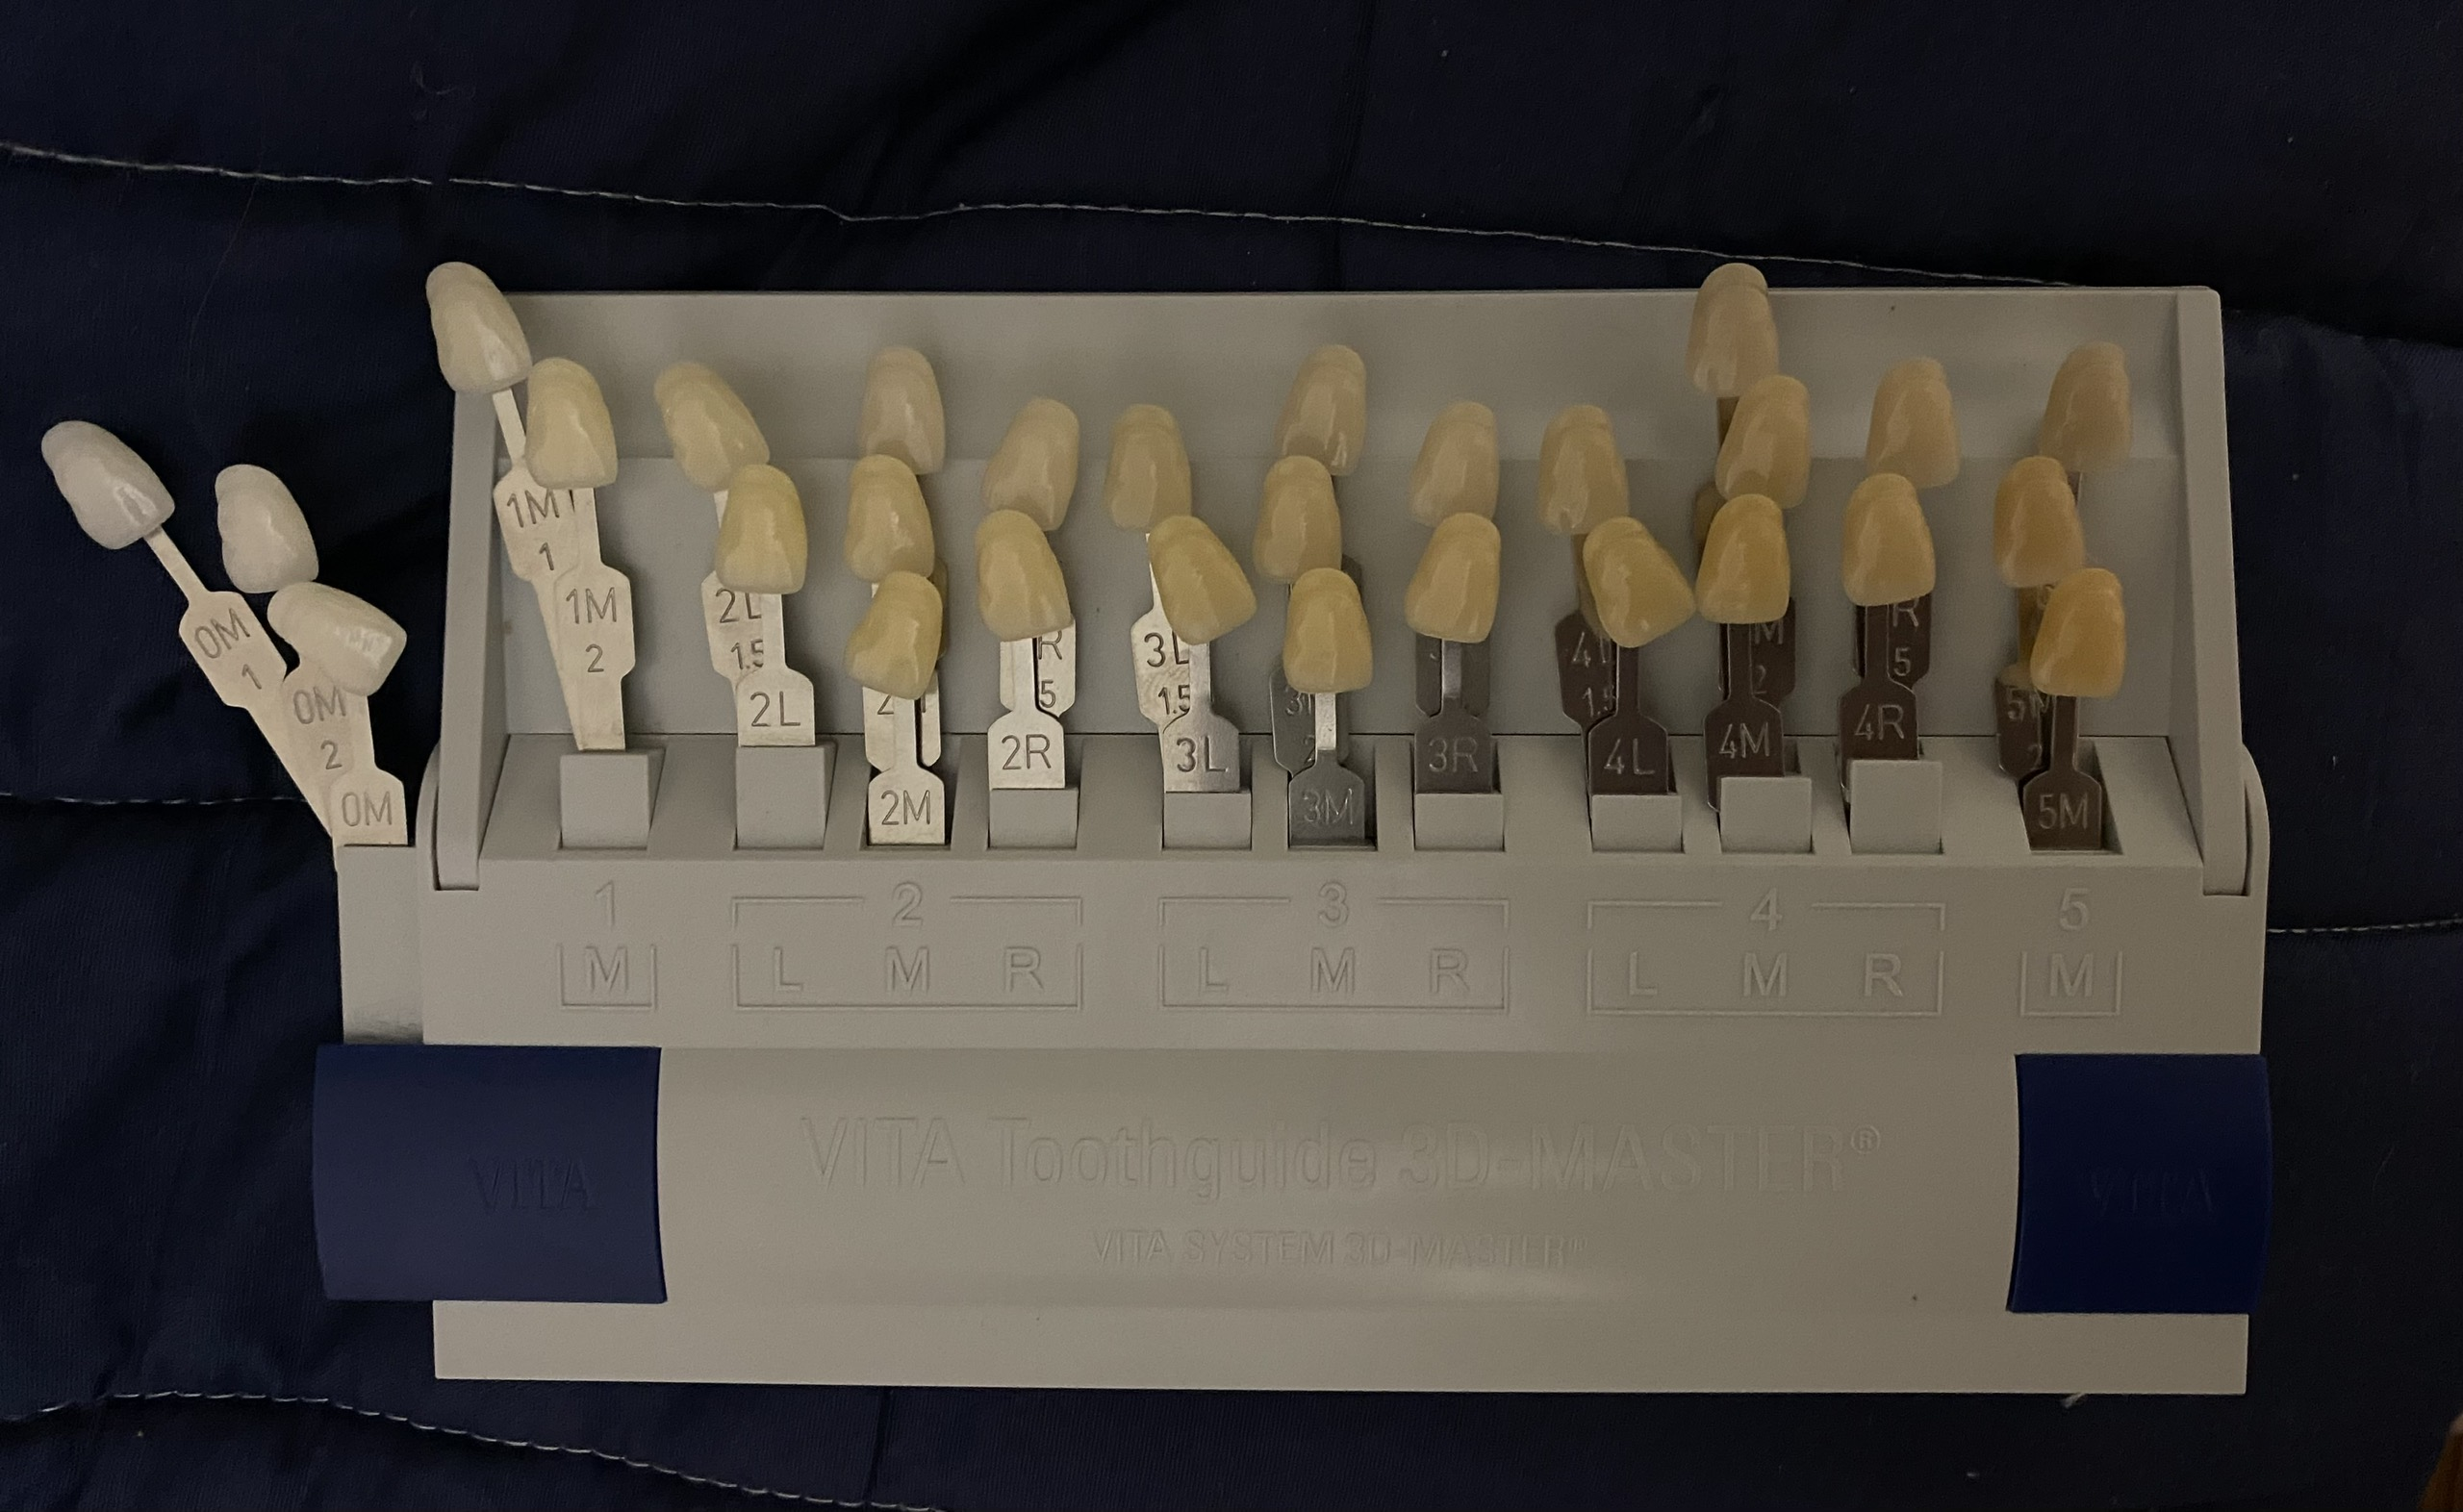
\includegraphics[width=0.7\columnwidth]{pictures/anh-bang-mau.jpeg}
    \caption {Ảnh bảng màu Vita 3D}
    \label{fig:anh-bang-mau}
    \end{figure}

\quad Bảng so màu Vita 3D được thiết kế theo ký hiệu theo thứ tự số - chữ cái - số (ví dụ 3M2), trong đó thể hiện theo thứ tự giá trị của Value, Chroma và Hue. Theo thứ tự value, chia thành 5 nhóm có giá trị value giảm dần từ nhóm 0 đến nhóm 5:\par
\quad Nhóm 0: Nhóm có value cao nhất, chỉ có một hue ký hiệu M (màu trung tính) có 3 cây 0M1, 0M2, 0M3 theo thứ tự tăng dần chroma từ nhạt đến sẫm màu hơn 0M1<0M2<0M3.\par
\quad Nhóm 1: 2 cây 1M1 và 1M2, có cùng hue màu trung tính ký hiệu M, có thứ tự tăng dần chroma 1M1<1M2.\par 
\quad Nhóm 2, 3 và 4: Có 7 cây, chia thành 3 phân nhóm nhỏ theo thứ tự thay đổi hue gồm: nhóm L (left) - màu vàng, nhóm M (medium) - màu trung tính, nhóm R (right) - màu đỏ. Trong nhóm L, độ chroma tăng dần 2L1<2L2; 3L1<3L2; 4L1<4L2. Trong nhóm M, độ chroma tăng dần 2M1<2M2<2M3; 3M1<3M2<3M3; 4M1<4M2<4M3. Trong nhóm R, độ chroma tăng dần 2R1<2R2; 3R1<3R2; 4R1<4R2.\par
\quad Nhóm 5: Có 3 cây, nhóm có value thấp nhất, chỉ có một hue ký hiệu M tương tự nhóm 0 (màu trung tính), 3 cây gồm 5M1, 5M2, 5M3 theo thứ tự tăng dần chroma 5M1<5M2<5M3.\par

\subsection{Lập phiếu thu thập thông tin}
\qquad Theo phụ lục 1

\subsection{Khám lâm sàng}
\textit{
\qquad Thực hiện so màu răng theo các bước sau:}\par
\begin{enumerate}
\setlength{\itemsep}{0pt}
\item Bước 1: Chọn value (Xác định độ sáng tối), chọn một trong năm nhóm sao cho độ sáng tối của răng giống nhất với độ sáng tối của các cây loại M trong bảng so màu từ nhóm value đã chọn được.
Giữ bảng so màu trên tay cạnh miệng bệnh nhân (đặt bên phải)
Chọn nhóm 0, 1, 2, 3, 4 hoặc 5 (0 là sáng nhất và 5 là tối nhất)
Bắt đầu so với với nhóm tối nhất trước.\par 
\item Bước 2: Chọn chroma (Chọn độ tương phản), dùng tông màu trung gian nhóm (M) để xác định độ tương phản bằng cách xòe que mẫu M như rẻ quạt. Chọn một trong ba màu sắc tương tự, gần giống nhất với răng được so màu.\par 
\item Bước 3: Chọn tông màu hue ( Kiểm trả xem răng tự nhiên vàng (bên trái L), trung tính (M) hay đỏ (bên phải R) hơn so với bảng màu: so sánh với các cây loại L và R có cùng nhóm với  cây loại M vừa chọn (cùng độ value và chroma), từ đó chọn ra cây có hue gần giống nhất với răng so màu, viết ký hiệu màu chọn theo quy ước của bảng so màu.\par 
\end{enumerate}
\textit{
\qquad So màu răng tuân thủ theo nguyên tắc sau đây:}\par 
\begin{itemize}
\setlength{\itemsep}{0pt}
    \item Đảm bảo đủ tiêu chuẩn về nguồn sáng, dùng ánh sáng hiệu chỉnh (color-corrected lighting) với nhiệt độ màu từ 5500 (D55) - 6500K (D65), chỉ số hoàn màu (color-rendering index) >=90; độ rọi (illuminance) từ 1000 đến 2000 lux, lý tưởng nhất dưới ánh sáng tự nhiên và đủ tiêu chuẩn kỹ thuật trên. Loại bỏ màu sắc gây nhiễu xung quanh răng so màu như son môi, đèn chiếu sáng khác, nên dùng nền tường không gian so màu là màu xám nhạt, tránh sử dụng màu sắc khác gây nhiễu loạn và mỏi mắt trước và trong khi so màu.\par 
\item Khi so màu, mắt người so màu để ngang mức răng, khoảng cách từ răng đến mắt khoảng từ 25-35cm (tương ứng 10-14 inch). Góc chiếu sáng và góc nhìn của người so màu phù hợp nhất là 45 độ/0 độ hoặc 0 độ/45 độ; mắt người quan sát thường ở vị trí trung tâm và nguồn chiếu sáng từ 1 hướng, 2 hướng và xung quanh.\par
\item Răng so màu cần được làm sạch, để ở trạng thái tự nhiên, không quá khô hoặc không quá ướt. Thời gian so màu từ 5-7 giây để tránh mỏi mắt và quen màu, tránh nhìn liên tục và cần cho mắt nghỉ ngơi, thời gian nghỉ ngơi tối thiểu là 5 phút, nên nhìn vào màu xám nhạt khi thư giãn mắt giữa những lần so màu.\par 
\item Vị trí đặt bảng so màu phụ thuộc vào phương pháp so màu và mục đích so màu, so màu pha macro thì đặt bảng so màu, sau đó chọn các cây tiếp tục cho pha sau như pha mini và pha micro.\par 
\item Đặt giữa răng hàm trên và hàm dưới hoặc kế bên ngang mức rìa cắn răng cần so màu, tránh đặt chồng lên phía trước hoặc phía sau răng cần so màu:\par 
\begin{itemize}
\setlength{\itemsep}{0pt}
\item Đặt đối đầu (rìa cắn - rìa cắn): Để so màu rìa cắn, nhưng không thể so màu cổ và thân răng.
\item Đặt cổ - rìa cắn: ít khi thực hiện.
\item Đặt nằm ngang: Để so màu thân răng.
\end{itemize}\par
\item Nếu đặt cây so màu bên cạnh răng cần so thì phải nghiêng tạo thành một góc 120 độ so với bề mặt răng thật, và quan sát từ hướng phân giác của góc này đến hai bề mặt răng thật và răng trên bảng so màu.\par 
\item Phương pháp so màu theo mô hình ba pha macro - mini - micro, bắt đầu bằng pha macro bằng cách sử dụng toàn bộ bảng so màu, chọn và đặt sang một bên các màu được lựa chọn để dùng cho pha sau, loại bỏ các màu không phù hợp. Ở pha mini, các cây được lựa chọn thì chọn tiếp sao cho phù hợp về màu của cổ, thân và rìa cắn gần nhất với răng cần so màu. Ở pha micro thì so sánh chi tiết về hue, value và chroma. Không đặt rìa cắn hướng về phía kim loại của bảng so màu.\par 
\item Nên so màu răng cả cùi răng và so màu từng phần của răng thành ba phần rìa cắn, thân và cổ răng. Nên thay đổi thêm góc độ để quan sát màu và nếu khó khăn trong việc quyết định màu thì nên mời thêm những chuyên gia khác cùng so màu và đưa ra kết luận chung một cách khách quan. Kết quả so màu cần ghi ký hiệu màu dưới dạng “ngôn ngữ màu (color language)” theo từng loại bảng so màu của nhà sản xuất nhằm thống nhất màu giữa bác sĩ và labo răng.\par 
\item Chụp hình màu được chọn nhằm tăng thêm dữ liệu đáng tin cậy cho sự giao tiếp màu giữa bác sĩ và labo, bác sĩ cần chụp ảnh kèm thêm hai màu gần nhất với màu được chọn đặt ở giữa so với hai màu lân cận (một màu sáng và một màu tối hơn so với màu được chọn). Đèn flash để chụp ảnh cần đảm bảo trong khoảng nhiệt trung tính (khoảng 5500K) để màu hình ảnh tự nhiên.\par

\end{itemize}

\vspace{-5pt}
\textbf{
\section{ Biến số, chỉ số nghiên cứu}}
\noindent
\textbf{Mục tiêu 1: Mô tả thực trạng nhiễm màu răng ở sinh viên trường đại học Y dược - Đại học Quốc gia Hà Nội năm 2023}

%chèn bảng biến số vô đây
\begin{longtable}{|l|l|l|l|l|} 
\hline
\textbf{STT} & \textbf{Biến số} & \textbf{Loại biến số} & \textbf{Định nghĩa biến} & \textbf{Phân tích}  \endfirsthead 
\hline
1            & Giới             & Định tính             & Nam hay nữ               & Tính tỷ lệ \%       \\ 
\hline
2            & Tuổi             & Định lượng            & Số tuổi                  & Tính tỷ lệ \%       \\ 
\hline
3            & Màu sắc răng     & Định tính             & Màu sắc răng             & Tính tỷ lệ \%       \\
\hline
\end{longtable}
\noindent
\textbf{Mục tiêu 2: Xác định nhu cầu điều trị ở nhóm đối tượng trên}

%chèn bảng biến số tiếp
\begin{longtblr}[
  label = none,
  entry = none,
]{
  width = \linewidth,
  colspec = {Q[54]Q[265]Q[138]Q[340]Q[127]},
  hlines,
  vlines,
}
\textbf{STT} & \textbf{Biến số}           & \textbf{Loại biến số} & \textbf{Định nghĩa biến}        & \textbf{Phân tích} \\
1            & Sự đổi màu răng            & Định tính             & Mức độ đổi màu răng             & Tính tỷ lệ \%      \\
2            & Vị trí phân bố đổi màu sắc & Định tính             & Vị trí phân bố vết đổi màu      & Tính tỷ lệ \%      \\
3            & Ảnh hưởng tới người bệnh   & Định tính~            & Mức độ ảnh hưởng tới người bệnh & Tính tỷ lệ \%      \\
4            & Nhu cầu làm trắng răng     & Định tính             & Nhu cầu làm trắng răng          & Tính tỷ lệ \%      
\end{longtblr}

\textbf{
\section{Đánh giá chỉ số nhu cầu làm trắng răng}}
\quad Chỉ số nhu cầu điều trị làm trắng răng được đánh giá theo Linda Greenwall như sau:\par
\noindent
\textbf{Loại 1 - Cao}
\begin{enumerate}
\setlength{\itemsep}{0pt}
    \item Sự đổi màu: nghiêm trọng
    \item Vị trí vết: phân bố nhiều đậm nhạt đồng đều
    \item Ảnh hưởng đến trẻ em: nghiêm trọng
    \item Nhu cầu làm trắng: cao
\end{enumerate}
\noindent
\textbf{Loại 2 - Trung bình}
\begin{enumerate}
\setlength{\itemsep}{0pt}
    \item Sự đổi màu: vừa phải
    \item Vị trí: phân bố đều
    \item Ảnh hưởng đến đứa trẻ: có ảnh hưởng đến đứa trẻ
    \item Nhu cầu làm trắng: vừa phải
\end{enumerate}
\noindent
\textbf{Loại 3 — Mong muốn}
\begin{enumerate}
\setlength{\itemsep}{0pt}
    \item Sự đổi màu: nhẹ
    \item Vị trí: ít răng trước
    \item Tác động đến trẻ em: một số tác động
    \item Nhu cầu làm trắng: mong muốn; điều này sẽ dễ dàng làm giảm bớt các vấn đề đổi màu
\end{enumerate}
\noindent
\textbf{Loại 4 — Khuyến cáo}
\begin{enumerate}
\setlength{\itemsep}{0pt}
    \item Sự đổi màu: các khu vực bị đổi màu bị cô lập
    \item Vị trí: phân bố ngẫu nhiên trên răng
    \item Ảnh hưởng đến trẻ em: vừa phải
    \item Nhu cầu làm trắng: khuyến cáo
\end{enumerate}
\noindent
\textbf{Loại 5 — Có thể}
\begin{enumerate}
\setlength{\itemsep}{0pt}
    \item Sự đổi màu: đổi màu nhẹ hoặc đốm trắng
    \item Vị trí: ít răng hoặc một răng
    \item Ảnh hưởng đến trẻ em: không ảnh hưởng đến trẻ em
    \item Nhu cầu làm trắng: có thể thực hiện được; có thể được mong muốn, nhưng có thể đợi cho đến khi đứa trẻ trên 18 tuổi.
\end{enumerate}

\vspace{-5pt}
\textbf{
\section{Thu thập dữ liệu}}
\quad Số liệu thu thập và phân tích bằng phương pháp thống kê y học, sử dụng phần mềm SPSS, Excel.\par
\quad Với mục tiêu 1 và 2: Mô tả đặc điểm màu sắc răng theo bảng màu Vita 3D Master và đánh giá nhu cầu làm trắng răng ở người bệnh: số liệu được trình bày bằng các bảng tần suất và các biểu đồ phù hợp.\par

\textbf{
\section{Đạo đức nghiên cứu}}
\quad Nghiên cứu được tiến hành khi hội đồng chấm đề cương thông qua và được sự đồng ý của Ban Giám Hiệu Trường Đại học Y Dược - Đại học Quốc gia Hà Nội.\par	
\quad Trước khi tiến hành nghiên cứu, giải thích đầy đủ cặn kẽ, chu đáo cho các người bệnh tham gia nghiên cứu. Người bệnh chấp thuận tham gia nghiên cứu và tự nguyện ký vào bản tham gia nghiên cứu.	\par
\quad Các thông tin thu thập được giữ bí mật, chỉ dùng với mục đích nghiên cứu. Nghiên cứu nhằm cải thiện thẩm mỹ và bảo vệ chăm sóc sức khỏe cho bệnh nhân mà không nhằm vào mục đích khác. \par
\vspace{-5pt}
\textbf{
\section{Sai số và biện pháp tránh sai số}}
\quad Khi so màu răng, có thể xảy ra sai số do nhiều yếu tố khác nhau như ánh sáng, góc nhìn, màu sắc tham chiếu và sự chủ quan của người quan sát. Tuyệt đối không thể loại trừ hoàn toàn sai số khi so màu răng, nhưng bằng cách tuân thủ những một số nguyên tắc sau giúp giảm sai số và đạt được kết quả gần đúng nhất trong quá trình so màu. để hạn chế sai số chúng tôi thực hiện như sau:\par
\quad Sử dụng điều kiện ánh sáng chuẩn: Đảm bảo răng được so màu trong điều kiện ánh sáng tự nhiên hoặc ánh sáng có màu sắc và cường độ đồng nhất. Tránh ánh sáng mạnh quá mức hoặc ánh sáng có màu sắc biến đổi có thể ảnh hưởng đến quá trình so màu.\par
\quad Đảm bảo môi trường không màu nhiễu: Tránh môi trường có màu sắc nổi bật hoặc quá phức tạp, vì nó có thể gây nhiễu và ảnh hưởng đến quá trình so màu. \par
\quad Một phòng chụp màu riêng biệt hoặc môi trường có màu trung lập có thể được sử dụng để giảm sai số.\par
\quad Sử dụng màu chuẩn ổn định: Chọn một bảng màu chuẩn hoặc màu sắc tham chiếu ổn định và được công nhận trong ngành nha khoa. Đảm bảo rằng màu chuẩn không bị mờ hoặc thay đổi màu theo thời gian.\par
\quad Đo và ghi lại màu sắc theo cách chuẩn: Sử dụng thiết bị đo màu nếu có thể để có kết quả chính xác và đáng tin cậy. Nếu sử dụng mắt thường, hãy cố gắng đánh giá màu sắc từ nhiều góc độ và so sánh với màu chuẩn càng cẩn thận càng tốt. Ghi lại màu sắc một cách chính xác và chi tiết để có thể so sánh và theo dõi sự thay đổi màu theo thời gian.\par
\quad Người so màu được huấn luyện về cách so màu so màu răng để giảm sai số. cần có thể có những kỹ năng và kinh nghiệm cần thiết để nhận biết và đánh giá màu sắc răng một cách chính xác.\par
\quad Kiểm tra lại kết quả với đánh giá thứ 2 và thảo luận: Kiểm tra lại kết quả so màu và thảo luận với người đánh giá thứ 2 để đảm bảo tính chính xác và đáng tin cậy của quá trình so màu.\par



\chapter{KẾT QUẢ NGHIÊN CỨU}

\textbf{
\section{Đặc điểm màu răng theo bảng Vita 3D ở sinh viên trường Đại học Y Dược - Đại học Quốc Gia Hà Nội năm 2023.}}


%chèn ảnh giới tính vào đây
\begin{figure}[h]
    \centering
    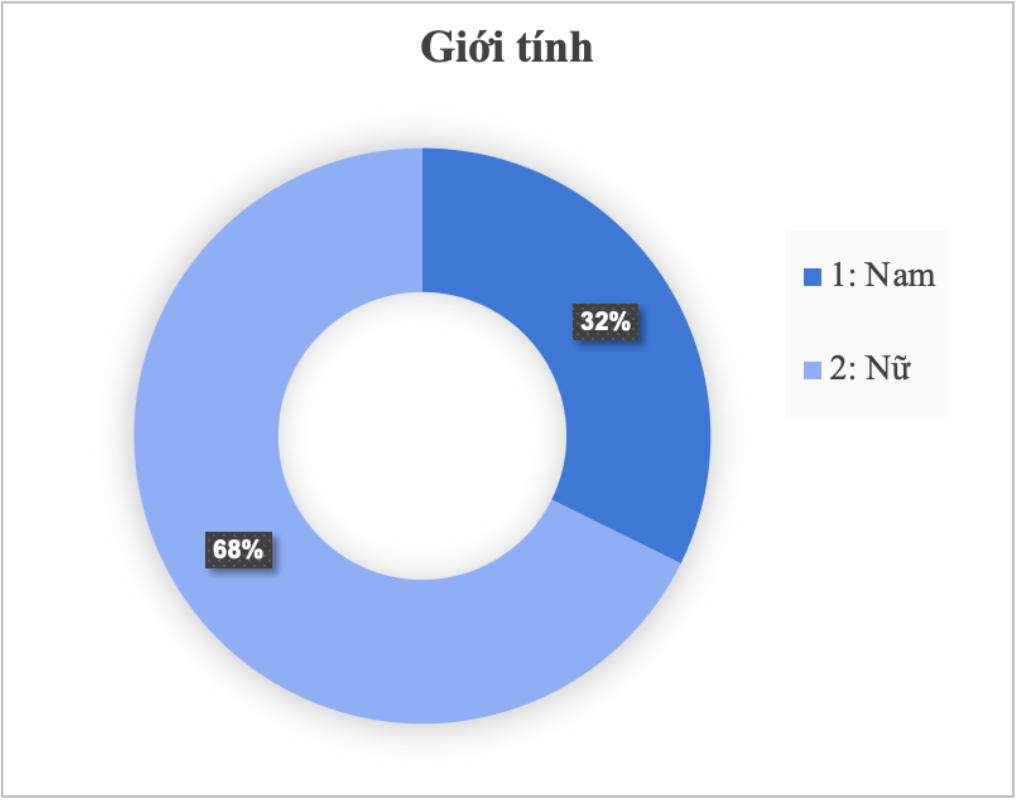
\includegraphics[width=0.8\columnwidth]{pictures/anh-gioi-tinh.jpeg}
    \caption{Biểu đồ tỷ lệ giới tính đối tượng nghiên cứu}
    \label{fig:yeu-to-chi-phoi-mau-sac-rang}
\end{figure}
\noindent
\textbf{Biểu đồ 3.1.1: Tỷ lệ nam nữ đối tượng nghiên cứu}

\noindent
\textbf{Nhận xét:}\par
\quad Tỷ lệ nữ cao gấp khoảng 2 lần so với nam.
\par

\noindent
\textbf{Bảng 3.1.1: Phân bố tiền sử người bệnh theo giới}
%chèn bảng vô đây
\begin{longtblr}[
caption=Phân bố tiền sử người bệnh theo giới
]{
  cells = {c},
  cell{1}{1} = {c=2,r=2}{},
  cell{1}{3} = {c=2}{},
  cell{1}{5} = {c=2}{},
  cell{1}{7} = {c=2}{},
  cell{3}{1} = {r=2}{},
  cell{5}{1} = {r=2}{},
  vlines,
  hline{1,3,5,7} = {-}{},
  hline{2} = {3-8}{},
  hline{4,6} = {2-8}{},
}
                                      &       & \textbf{Nam} &        & \textbf{Nữ} &        & \textbf{Tổng số} &        \\
                                      &       & n            & \%     & n           & \%     & n                & \%     \\
\textbf{Tiền sử sử dụng Tetracycline} & Không & 17           & 26,2\% & 34          & 52,3\% & 51               & 78,5\% \\
                                      & Có    & 4            & 6,2\%  & 10          & 15,4\% & 14               & 21,5\% \\
\textbf{Tiền sử chấn thương răng}     & Không & 20           & 30,8\% & 40          & 61,5\% & 60               & 92,3\% \\
                                      & Có    & 1            & 1,5\%  & 4           & 6,2\%  & 5                & 7,7\%  
\end{longtblr}
\vspace{1cm}
\noindent
\textbf{Nhận xét:}\par
\quad Tỷ lệ tiền sử sử dụng Tetracycline ở hai giới nam và nữ đều thấp (nữ: 21,5\% và nam: 6,2\%). Tỷ lệ có tiền sử chấn thương răng ở hai giới thấp (nữ: 7,7\% và nam: 1,5\%).\par

\noindent
\textbf{Bảng 3.1.2: Phân bố thói quen sử dụng đồ có màu của người bệnh theo giới}
%chèn bảng vô đây
\begin{longtblr}[
caption=Phân bố thói quen sử dụng đồ có màu của người bệnh theo giới
]{
  width = \linewidth,
  colspec = {Q[296]Q[92]Q[42]Q[106]Q[42]Q[106]Q[42]Q[106]Q[90]},
  row{even} = {c},
  row{3} = {c},
  row{5} = {c},
  row{7} = {c},
  row{9} = {c},
  row{11} = {c},
  cell{1}{1} = {c=2,r=2}{0.388\linewidth},
  cell{1}{3} = {c=2}{0.148\linewidth,c},
  cell{1}{5} = {c=2}{0.148\linewidth,c},
  cell{1}{7} = {c=2}{0.148\linewidth,c},
  cell{1}{9} = {r=2}{c},
  cell{3}{1} = {r=2}{},
  cell{3}{9} = {r=2}{},
  cell{5}{1} = {r=2}{},
  cell{5}{9} = {r=2}{},
  cell{7}{1} = {r=2}{},
  cell{7}{9} = {r=2}{},
  cell{9}{1} = {r=2}{},
  cell{9}{9} = {r=2}{},
  cell{11}{1} = {r=2}{},
  cell{11}{9} = {r=2}{},
  vlines,
  hline{1,3,5,7,9,11,13} = {-}{},
  hline{2} = {3-8}{},
  hline{4,6,8,10,12} = {2-8}{},
}
                           &       & \textbf{Nam} &         & \textbf{Nữ} &         & \textbf{Tổng số} &         & \textbf{P} \\
                           &       & n            & \%      & n           & \%      & n                & \%      &            \\
\textbf{Hút thuốc}         & Không & 15           & 23,10\% & 44          & 67,70\% & 59               & 90,80\% &  <0,01      \\
                           & Có    & 6            & 9,20\%  & 0           & 0,00\%  & 6                & 9,20\%  &            \\
\textbf{Cà phê}            & Không & 9            & 13,80\% & 26          & 40,00\% & 35               & 53,80\% &  >0,05      \\
                           & Có    & 12           & 18,50\% & 18          & 27,70\% & 30               & 46,20\% &            \\
\textbf{Nước chè}          & Không & 15           & 23,10\% & 38          & 58,50\% & 53               & 81,50\% &  >0,05      \\
                           & Có    & 6            & 9,20\%  & 6           & 9,20\%  & 12               & 18,50\% &            \\
\textbf{Coca Cola}         & Không & 5            & 7,70\%  & 21          & 32,30\% & 26               & 40,00\% &  >0,05      \\
                           & Có    & 16           & 24,60\% & 23          & 35,40\% & 39               & 60,00\% &            \\
\textbf{Nước uống sẫm màu} & Không & 6            & 9,20\%  & 30          & 46,20\% & 36               & 55,40\% &  <0,05      \\
                           & Có    & 15           & 23,10\% & 14          & 21,50\% & 29               & 44,60\% &            
\end{longtblr}
%đến đây là kết thúc bảng ạ

\noindent
\textbf{Nhận xét:}\par
\quad Thói quen sử dụng đồ có màu, cà phê, coca cola ở cả hai giới không có sự khác biệt nhiều (p>0,05). \par
\quad Thói quen sử dụng cocacola là cao nhất (60\%), uống cà phê chiếm 46,2\%, và đồ uống có màu khác chiếm khoảng 44,6\%. Hút thuốc lá chiếm 9,2\%. Hút thuốc lá chỉ gặp ở nam giới, không gặp ở nữ giới.


\noindent
\textbf{Bảng 3.1.3: Phân bố tình trạng vệ sinh răng miệng của người bệnh theo giới}\par

%chèn bảng vô đây
\begin{longtblr}[
caption=Phân bố tình trạng vệ sinh răng miệng của người bệnh theo giới
]{
  width = \linewidth,
  colspec = {Q[212]Q[302]Q[38]Q[79]Q[38]Q[79]Q[38]Q[79]Q[67]},
  row{2} = {c},
  column{2} = {c},
  column{9} = {c},
  cell{1}{1} = {c=2,r=2}{0.514\linewidth},
  cell{1}{3} = {c=2}{0.117\linewidth,c},
  cell{1}{5} = {c=2}{0.117\linewidth,c},
  cell{1}{7} = {c=2}{0.117\linewidth,c},
  cell{1}{9} = {r=2}{},
  cell{3}{1} = {r=3}{c},
  cell{3}{3} = {c},
  cell{3}{4} = {c},
  cell{3}{5} = {c},
  cell{3}{6} = {c},
  cell{3}{9} = {r=3}{},
  cell{4}{3} = {c},
  cell{4}{4} = {c},
  cell{4}{5} = {c},
  cell{4}{6} = {c},
  cell{5}{3} = {c},
  cell{5}{4} = {c},
  cell{5}{5} = {c},
  cell{5}{6} = {c},
  cell{6}{1} = {r=2}{c},
  cell{6}{3} = {c},
  cell{6}{4} = {c},
  cell{6}{5} = {c},
  cell{6}{6} = {c},
  cell{6}{9} = {r=2}{},
  cell{7}{3} = {c},
  cell{7}{4} = {c},
  cell{7}{5} = {c},
  cell{7}{6} = {c},
  cell{8}{1} = {r=4}{c},
  cell{8}{3} = {c},
  cell{8}{4} = {c},
  cell{8}{5} = {c},
  cell{8}{6} = {c},
  cell{8}{9} = {r=4}{},
  cell{9}{3} = {c},
  cell{9}{4} = {c},
  cell{9}{5} = {c},
  cell{9}{6} = {c},
  cell{10}{3} = {c},
  cell{10}{4} = {c},
  cell{10}{5} = {c},
  cell{10}{6} = {c},
  cell{11}{3} = {c},
  cell{11}{4} = {c},
  cell{11}{5} = {c},
  cell{11}{6} = {c},
  vlines,
  hline{1,3,6,8,12} = {-}{},
  hline{2} = {3-8}{},
  hline{4-5,7,9-11} = {2-8}{},
}
                              &                                  & \textbf{Nam} &        & \textbf{Nữ} &        & \textbf{Tổng số} &        & \textbf{P} \\
                              &                                  & n            & \%     & n           & \%     & n                & \%     &            \\
\textbf{Vệ sinh răng miệng}   & 1 lần/ngày                       & 0            & 0,0\%  & 0           & 0,0\%  & 0                & 0,0\%  & > 0,05       \\
                              & 2 lần/ngày                       & 17           & 26,2\% & 36          & 55,4\% & 53               & 81,5\% &            \\
                              & trên 2 lần/ngày                  & 4            & 6,2\%  & 8           & 12,3\% & 12               & 18,5\% &            \\
\textbf{Nước súc miệng}       & Không                           & 15           & 23,1\% & 32          & 49,2\% & 47               & 72,3\% & > 0,05       \\
                              & Có                               & 6            & 9,2\%  & 12          & 18,5\% & 18               & 27,7\% &            \\
\textbf{Lấy cao răng định kì} & Chưa bao giờ lấy cao răng        & 4            & 6,2\%  & 8           & 12,3\% & 12               & 18,5\% & > 0,05       \\
                              & Lấy cao răng 3 tháng 1 lần       & 0            & 0,0\%  & 4           & 6,2\%  & 4                & 6,2\%  &            \\
                              & Lấy cao 6 tháng 1 lần            & 12           & 18,5\% & 18          & 27,7\% & 30               & 46,2\% &            \\
                              & Trên 1 năm đi lấy cao răng 1 lần & 5            & 7,7\%  & 14          & 21,5\% & 19               & 29,2\% &            
\end{longtblr}

\noindent
\textbf{Nhận xét:}\par
\quad Tình trạng vệ sinh răng miệng ở hai giới tương đối đồng đều. \par
\quad Vệ sinh răng miệng 2 lần/ngày cao nhất, chiếm khoảng 81,5\%, không có ý nghĩa thống kê (p>0,05).\par
\quad Tỷ lệ sử dụng nước súc miệng có màu sẫm tương đối thấp, khoảng 27,7\%. \par
\quad Tình trạng chăm sóc răng miệng định kỳ 6 tháng 1 lần chiếm tỷ lệ khoảng 46,2\%. \par
\quad Tỷ lệ trên 1 năm đi lấy cao răng 1 lần chiếm khoảng 29,2\%. Chưa đi lấy cao răng bao giờ chiếm tỷ lệ 18,5\% và không có ý nghĩa thống kê (p>0,05).

\noindent
\textbf{Bảng 3.1.4: Phân bố đặc điểm của răng theo giới}\par

%chèn bảng vô đây
\begin{longtblr}[
caption=Phân bố đặc điểm của răng theo giới
]{
  width = \linewidth,
  colspec = {Q[202]Q[225]Q[42]Q[90]Q[42]Q[90]Q[42]Q[106]Q[83]},
  row{2} = {c},
  column{2} = {c},
  column{9} = {c},
  cell{1}{1} = {c=2,r=2}{0.427\linewidth},
  cell{1}{3} = {c=2}{0.132\linewidth,c},
  cell{1}{5} = {c=2}{0.132\linewidth,c},
  cell{1}{7} = {c=2}{0.148\linewidth,c},
  cell{1}{9} = {r=2}{},
  cell{3}{1} = {r=2}{c},
  cell{3}{3} = {c},
  cell{3}{4} = {c},
  cell{3}{5} = {c},
  cell{3}{6} = {c},
  cell{3}{9} = {r=2}{},
  cell{4}{3} = {c},
  cell{4}{4} = {c},
  cell{4}{5} = {c},
  cell{4}{6} = {c},
  cell{5}{1} = {r=2}{c},
  cell{5}{3} = {c},
  cell{5}{4} = {c},
  cell{5}{5} = {c},
  cell{5}{6} = {c},
  cell{5}{9} = {r=2}{},
  cell{6}{3} = {c},
  cell{6}{4} = {c},
  cell{6}{5} = {c},
  cell{6}{6} = {c},
  cell{7}{1} = {r=2}{c},
  cell{7}{3} = {c},
  cell{7}{4} = {c},
  cell{7}{5} = {c},
  cell{7}{6} = {c},
  cell{7}{9} = {r=2}{},
  cell{8}{3} = {c},
  cell{8}{4} = {c},
  cell{8}{5} = {c},
  cell{8}{6} = {c},
  cell{9}{1} = {r=2}{c},
  cell{9}{3} = {c},
  cell{9}{4} = {c},
  cell{9}{5} = {c},
  cell{9}{6} = {c},
  cell{9}{9} = {r=2}{},
  cell{10}{3} = {c},
  cell{10}{4} = {c},
  cell{10}{5} = {c},
  cell{10}{6} = {c},
  vlines,
  hline{1,3,5,7,9,11} = {-}{},
  hline{2} = {3-8}{},
  hline{4,6,8,10} = {2-8}{},
}
                       &                 & \textbf{Nam} &        & \textbf{Nữ} &        & \textbf{Tổng số} &         & \textbf{P} \\
                       &                 & n            & \%     & n           & \%     & n                & \%      &             \\
\textbf{Bề mặt răng}   & Nhẵn bóng       & 20           & 30,8\% & 40          & 61,5\% & 60               & 92,3\%  & >0,05        \\
                       & Sần sùi         & 1            & 1,5\%  & 4           & 6,2\%  & 5                & 7,7\%   &             \\
\textbf{Răng rạn nứt}  & Không           & 21           & 32,3\% & 43          & 66,2\% & 64               & 98,5\%  & >0,05        \\
                       & Có              & 0            & 0,0\%  & 1           & 1,5\%  & 1                & 1,5\%   &             \\
\textbf{Răng sâu}      & Không           & 21           & 32,3\% & 44          & 67,7\% & 65               & 100,0\% & 0           \\
                       & Có              & 0            & 0,0\%  & 0           & 0,0\%  & 0                & 0,0\%   &             \\
\textbf{Tính chất màu} & {Không đồng \\ nhất} & 1            & 1,5\%  & 7           & 10,8\% & 8                & 12,3\%  & >0,05        \\
                       & Đồng nhất       & 20           & 30,8\% & 37          & 56,9\% & 57               & 87,7\%  &             
\end{longtblr}

\noindent
\textbf{Nhận xét:}\par
\quad Tỷ lệ bề mặt răng nhẵn bóng (92,3\%) cao hơn so với bề mặt răng sần sùi (7,7\%), không có ý nghĩa thống kê (p>0,05). Đa số các răng không rạn nứt (98,5\%), không có ý nghĩa thống kê (p>0,05). Không có răng sâu nào. Tỷ lệ tính chất màu sắc răng đồng nhất là 87,7\%, cao hơn tỷ lệ tính chất màu sắc răng không đồng nhất khoảng 7 lần (12,3\%), không có ý nghĩa thống kê (p>0,05).\\
\noindent
\textbf{Bảng 3.1.5: Phân bố màu sắc giá trị màu (value) hàm trên theo nhóm răng}\par

\begin{longtblr}[
caption=Phân bố màu sắc giá trị màu (value) hàm trên theo nhóm răng
]{
  row{2} = {c},
  column{2} = {c},
  column{9} = {c},
  cell{1}{1} = {c=2,r=2}{},
  cell{1}{3} = {c=2}{c},
  cell{1}{5} = {c=2}{c},
  cell{1}{7} = {c=2}{c},
  cell{1}{9} = {r=2}{},
  cell{3}{1} = {r=5}{c},
  cell{3}{3} = {c},
  cell{3}{4} = {c},
  cell{3}{5} = {c},
  cell{3}{6} = {c},
  cell{3}{9} = {r=5}{},
  cell{4}{3} = {c},
  cell{4}{4} = {c},
  cell{4}{5} = {c},
  cell{4}{6} = {c},
  cell{5}{3} = {c},
  cell{5}{4} = {c},
  cell{5}{5} = {c},
  cell{5}{6} = {c},
  cell{6}{3} = {c},
  cell{6}{4} = {c},
  cell{6}{5} = {c},
  cell{6}{6} = {c},
  cell{7}{3} = {c},
  cell{7}{4} = {c},
  cell{7}{5} = {c},
  cell{7}{6} = {c},
  cell{8}{1} = {r=5}{c},
  cell{8}{3} = {c},
  cell{8}{4} = {c},
  cell{8}{5} = {c},
  cell{8}{6} = {c},
  cell{8}{9} = {r=5}{},
  cell{9}{3} = {c},
  cell{9}{4} = {c},
  cell{9}{5} = {c},
  cell{9}{6} = {c},
  cell{10}{3} = {c},
  cell{10}{4} = {c},
  cell{10}{5} = {c},
  cell{10}{6} = {c},
  cell{11}{3} = {c},
  cell{11}{4} = {c},
  cell{11}{5} = {c},
  cell{11}{6} = {c},
  cell{12}{3} = {c},
  cell{12}{4} = {c},
  cell{12}{5} = {c},
  cell{12}{6} = {c},
  cell{13}{1} = {r=5}{c},
  cell{13}{3} = {c},
  cell{13}{4} = {c},
  cell{13}{5} = {c},
  cell{13}{6} = {c},
  cell{13}{9} = {r=5}{},
  cell{14}{3} = {c},
  cell{14}{4} = {c},
  cell{14}{5} = {c},
  cell{14}{6} = {c},
  cell{15}{3} = {c},
  cell{15}{4} = {c},
  cell{15}{5} = {c},
  cell{15}{6} = {c},
  cell{16}{3} = {c},
  cell{16}{4} = {c},
  cell{16}{5} = {c},
  cell{16}{6} = {c},
  cell{17}{3} = {c},
  cell{17}{4} = {c},
  cell{17}{5} = {c},
  cell{17}{6} = {c},
  vlines,
  hline{1,3,8,13,18} = {-}{},
  hline{2} = {3-8}{},
  hline{4-7,9-12,14-17} = {2-8}{},
}
                                &        & \textbf{Nam} &        & \textbf{Nữ} &        & \textbf{Tổng số} &        & P    \\
                                &        & n            & \%     & n           & \%     & n                & \%     &      \\
\textbf{Nhóm răng cửa trên}     & Nhóm 1 & 0            & 0,0\%  & 1           & 1,5\%  & 1                & 1,5\%  & >0,05 \\
                                & Nhóm 2 & 9            & 13,8\% & 19          & 29,2\% & 28               & 43,1\% &      \\
                                & Nhóm 3 & 10           & 15,4\% & 23          & 35,4\% & 33               & 50,8\% &      \\
                                & Nhóm 4 & 2            & 3,1\%  & 1           & 1,5\%  & 3                & 4,6\%  &      \\
                                & Nhóm 5 & 0            & 0,0\%  & 0           & 0,0\%  & 0                & 0,0\%  &      \\
\textbf{Nhóm răng nanh trên}    & Nhóm 1 & 0            & 0,0\%  & 0           & 0,0\%  & 0                & 0,0\%  & >0,05 \\
                                & Nhóm 2 & 7            & 10,8\% & 19          & 29,2\% & 26               & 40,0\% &      \\
                                & Nhóm 3 & 11           & 16,9\% & 24          & 36,9\% & 35               & 53,8\% &      \\
                                & Nhóm 4 & 3            & 4,6\%  & 1           & 1,5\%  & 4                & 6,2\%  &      \\
                                & Nhóm 5 & 0            & 0,0\%  & 0           & 0,0\%  & 0                & 0,0\%  &      \\
\textbf{Nhóm răng hàm nhỏ trên} & Nhóm 1 & 0            & 0,0\%  & 1           & 1,5\%  & 1                & 1,5\%  & >0,05 \\
                                & Nhóm 2 & 8            & 12,3\% & 19          & 29,2\% & 27               & 41,5\% &      \\
                                & Nhóm 3 & 11           & 16,9\% & 24          & 36,9\% & 35               & 53,8\% &      \\
                                & Nhóm 4 & 2            & 3,1\%  & 0           & 0,0\%  & 2                & 3,1\%  &      \\
                                & Nhóm 5 & 0            & 0,0\%  & 0           & 0,0\%  & 0                & 0,0\%  &      
\end{longtblr}
%chèn bảng vô đây

\noindent
\textbf{Nhận xét:}\par
\quad Tỷ lệ phân bố màu sắc răng giá trị màu ở nhóm 3 là cao nhất ở cả 3 nhóm răng (nhóm răng cửa (50,8\%), nhóm răng nanh (53,8\%), nhóm răng hàm nhỏ (53,8\%)) và tương đối ngang nhau giữa hai giới nam và nữ (p>0,05).\par
\quad Tỷ lệ giá trị màu sắc răng ở nhóm 2 xếp sau với nhóm răng cửa khoảng 43\%, nhóm răng nanh khoảng 40\% và nhóm răng hàm nhỏ khoảng 41,5\%.\par
\quad Nhóm 1 chỉ chiếm tỷ lệ rất nhỏ là 1,5\% và không có đối tượng nào có màu sắc theo nhóm 5. Không có ý nghĩa thống kê (p>0,05).

\noindent
\textbf{Bảng 3.1.6: Phân bố màu sắc giá trị màu (value) hàm dưới theo nhóm răng
}\par
\begin{longtblr}[
caption=Phân bố màu sắc giá trị màu (value) hàm dưới theo nhóm răng
]{
  row{2} = {c},
  column{2} = {c},
  column{9} = {c},
  cell{1}{1} = {c=2,r=2}{},
  cell{1}{3} = {c=2}{c},
  cell{1}{5} = {c=2}{c},
  cell{1}{7} = {c=2}{c},
  cell{1}{9} = {r=2}{},
  cell{3}{1} = {r=5}{c},
  cell{3}{3} = {c},
  cell{3}{4} = {c},
  cell{3}{5} = {c},
  cell{3}{6} = {c},
  cell{3}{9} = {r=5}{},
  cell{4}{3} = {c},
  cell{4}{4} = {c},
  cell{4}{5} = {c},
  cell{4}{6} = {c},
  cell{5}{3} = {c},
  cell{5}{4} = {c},
  cell{5}{5} = {c},
  cell{5}{6} = {c},
  cell{6}{3} = {c},
  cell{6}{4} = {c},
  cell{6}{5} = {c},
  cell{6}{6} = {c},
  cell{7}{3} = {c},
  cell{7}{4} = {c},
  cell{7}{5} = {c},
  cell{7}{6} = {c},
  cell{8}{1} = {r=5}{c},
  cell{8}{3} = {c},
  cell{8}{4} = {c},
  cell{8}{5} = {c},
  cell{8}{6} = {c},
  cell{8}{9} = {r=5}{},
  cell{9}{3} = {c},
  cell{9}{4} = {c},
  cell{9}{5} = {c},
  cell{9}{6} = {c},
  cell{10}{3} = {c},
  cell{10}{4} = {c},
  cell{10}{5} = {c},
  cell{10}{6} = {c},
  cell{11}{3} = {c},
  cell{11}{4} = {c},
  cell{11}{5} = {c},
  cell{11}{6} = {c},
  cell{12}{3} = {c},
  cell{12}{4} = {c},
  cell{12}{5} = {c},
  cell{12}{6} = {c},
  cell{13}{1} = {r=5}{c},
  cell{13}{3} = {c},
  cell{13}{4} = {c},
  cell{13}{5} = {c},
  cell{13}{6} = {c},
  cell{13}{9} = {r=5}{},
  cell{14}{3} = {c},
  cell{14}{4} = {c},
  cell{14}{5} = {c},
  cell{14}{6} = {c},
  cell{15}{3} = {c},
  cell{15}{4} = {c},
  cell{15}{5} = {c},
  cell{15}{6} = {c},
  cell{16}{3} = {c},
  cell{16}{4} = {c},
  cell{16}{5} = {c},
  cell{16}{6} = {c},
  cell{17}{3} = {c},
  cell{17}{4} = {c},
  cell{17}{5} = {c},
  cell{17}{6} = {c},
  vlines,
  hline{1,3,8,13,18} = {-}{},
  hline{2} = {3-8}{},
  hline{4-7,9-12,14-17} = {2-8}{},
}
                                &        & \textbf{Nam} &        & \textbf{Nữ} &        & \textbf{Tổng số} &        & \textbf{P} \\
                                &        & n            & \%     & n           & \%     & n                & \%     &            \\
\textbf{Nhóm răng cửa dưới}     & Nhóm 1 & 0            & 0,0\%  & 0           & 0,0\%  & 0                & 0,0\%  & <0,05       \\
                                & Nhóm 2 & 6            & 9,4\%  & 11          & 17,2\% & 17               & 26,6\% &            \\
                                & Nhóm 3 & 12           & 18,8\% & 32          & 50,0\% & 44               & 68,8\% &            \\
                                & Nhóm 4 & 3            & 4,7\%  & 0           & 0,0\%  & 3                & 4,7\%  &            \\
                                & Nhóm 5 & 0            & 0,0\%  & 0           & 0,0\%  & 0                & 0,0\%  &            \\
\textbf{Nhóm răng nanh dưới}    & Nhóm 1 & 0            & 0,0\%  & 0           & 0,0\%  & 0                & 0,0\%  & >0,05       \\
                                & Nhóm 2 & 5            & 7,8\%  & 11          & 17,2\% & 16               & 25,0\% &            \\
                                & Nhóm 3 & 11           & 17,2\% & 28          & 43,8\% & 39               & 60,9\% &            \\
                                & Nhóm 4 & 5            & 7,8\%  & 4           & 6,3\%  & 9                & 14,1\% &            \\
                                & Nhóm 5 & 0            & 0,0\%  & 0           & 0,0\%  & 0                & 0,0\%  &            \\
\textbf{Nhóm răng hàm nhỏ dưới} & Nhóm 1 & 0            & 0,0\%  & 0           & 0,0\%  & 0                & 0,0\%  & <0,05       \\
                                & Nhóm 2 & 5            & 7,8\%  & 11          & 17,2\% & 16               & 25,0\% &            \\
                                & Nhóm 3 & 13           & 20,3\% & 32          & 50,0\% & 45               & 70,3\% &            \\
                                & Nhóm 4 & 3            & 4,7\%  & 0           & 0,0\%  & 3                & 4,7\%  &            \\
                                & Nhóm 5 & 0            & 0,0\%  & 0           & 0,0\%  & 0                & 0,0\%  &            
\end{longtblr}
%chèn bảng vô đây

\noindent
\textbf{Nhận xét:}\par
\quad Tỷ lệ phân bố giá trị màu sắc răng ở nhóm 3 là cao nhất ở cả 3 nhóm răng (nhóm răng cửa (68,8\%), nhóm răng nanh (6\%), nhóm răng hàm nhỏ(70,3\%)) và tương đối ngang nhau giữa hai giới nam và nữ. \par
\quad Tỷ lệ giá trị màu sắc răng ở nhóm 2 xếp sau với nhóm răng cửa khoảng 26,6\%, nhóm răng nanh khoảng 25\% và nhóm răng hàm nhỏ khoảng 25\%. Nhóm 1 và nhóm 5 không có đối tượng nào.\par
\quad Tỷ lệ phân bố màu sắc răng ở nhóm răng cửa dưới và nhóm răng hàm nhỏ dưới là có ý nghĩa thống kê (p<0,05) còn ở nhóm răng nanh dưới không có ý nghĩa thống kê (p>0,05).

\noindent
\textbf{Bảng 3.1.7: Phân bố màu sắc răng theo độ bão hoà và nhóm răng}\par

%chèn bảng vô đây
\begin{longtblr}[
caption=Phân bố màu sắc răng theo độ bão hoà và nhóm răng
]{
  row{2} = {c},
  column{2} = {c},
  column{9} = {c},
  cell{1}{1} = {c=2,r=2}{},
  cell{1}{3} = {c=2}{c},
  cell{1}{5} = {c=2}{c},
  cell{1}{7} = {c=2}{c},
  cell{1}{9} = {r=2}{},
  cell{3}{1} = {r=3}{c},
  cell{3}{3} = {c},
  cell{3}{4} = {c},
  cell{3}{5} = {c},
  cell{3}{6} = {c},
  cell{3}{9} = {r=3}{},
  cell{4}{3} = {c},
  cell{4}{4} = {c},
  cell{4}{5} = {c},
  cell{4}{6} = {c},
  cell{5}{3} = {c},
  cell{5}{4} = {c},
  cell{5}{5} = {c},
  cell{5}{6} = {c},
  cell{6}{1} = {r=3}{c},
  cell{6}{3} = {c},
  cell{6}{4} = {c},
  cell{6}{5} = {c},
  cell{6}{6} = {c},
  cell{6}{9} = {r=3}{},
  cell{7}{3} = {c},
  cell{7}{4} = {c},
  cell{7}{5} = {c},
  cell{7}{6} = {c},
  cell{8}{3} = {c},
  cell{8}{4} = {c},
  cell{8}{5} = {c},
  cell{8}{6} = {c},
  cell{9}{1} = {r=3}{c},
  cell{9}{3} = {c},
  cell{9}{4} = {c},
  cell{9}{5} = {c},
  cell{9}{6} = {c},
  cell{9}{9} = {r=3}{},
  cell{10}{3} = {c},
  cell{10}{4} = {c},
  cell{10}{5} = {c},
  cell{10}{6} = {c},
  cell{11}{3} = {c},
  cell{11}{4} = {c},
  cell{11}{5} = {c},
  cell{11}{6} = {c},
  cell{12}{1} = {r=3}{c},
  cell{12}{3} = {c},
  cell{12}{4} = {c},
  cell{12}{5} = {c},
  cell{12}{6} = {c},
  cell{12}{9} = {r=3}{},
  cell{13}{3} = {c},
  cell{13}{4} = {c},
  cell{13}{5} = {c},
  cell{13}{6} = {c},
  cell{14}{3} = {c},
  cell{14}{4} = {c},
  cell{14}{5} = {c},
  cell{14}{6} = {c},
  cell{15}{1} = {r=3}{c},
  cell{15}{3} = {c},
  cell{15}{4} = {c},
  cell{15}{5} = {c},
  cell{15}{6} = {c},
  cell{15}{9} = {r=3}{},
  cell{16}{3} = {c},
  cell{16}{4} = {c},
  cell{16}{5} = {c},
  cell{16}{6} = {c},
  cell{17}{3} = {c},
  cell{17}{4} = {c},
  cell{17}{5} = {c},
  cell{17}{6} = {c},
  cell{18}{1} = {r=3}{c},
  cell{18}{3} = {c},
  cell{18}{4} = {c},
  cell{18}{5} = {c},
  cell{18}{6} = {c},
  cell{18}{9} = {r=3}{},
  cell{19}{3} = {c},
  cell{19}{4} = {c},
  cell{19}{5} = {c},
  cell{19}{6} = {c},
  cell{20}{3} = {c},
  cell{20}{4} = {c},
  cell{20}{5} = {c},
  cell{20}{6} = {c},
  vlines,
  hline{1,3,6,9,12,15,18,21} = {-}{},
  hline{2} = {3-8}{},
  hline{4-5,7-8,10-11,13-14,16-17,19-20} = {2-8}{},
}
                                &   & \textbf{Nam} &        & \textbf{Nữ} &        & \textbf{Tổng số} &        & P    \\
                                &   & n             & \%     & n           & \%     & n                & \%     &      \\
\textbf{Nhóm răng cửa trên}     & L & 2             & 3,1\%  & 2           & 3,1\%  & 4                & 6,2\%  & >0,05 \\
                                & M & 13            & 20,0\% & 21          & 32,3\% & 34               & 52,3\% &      \\
                                & R & 6             & 9,2\%  & 21          & 32,3\% & 27               & 41,5\% &      \\
\textbf{Nhóm răng nanh trên}    & L & 3             & 4,6\%  & 6           & 9,2\%  & 9                & 13,8\% & >0,05 \\
                                & M & 13            & 20,0\% & 30          & 46,2\% & 43               & 66,2\% &      \\
                                & R & 5             & 7,7\%  & 8           & 12,3\% & 13               & 20,0\% &      \\
\textbf{Nhóm răng hàm nhỏ trên} & L & 4             & 6,2\%  & 3           & 4,6\%  & 7                & 10,8\% & >0,05 \\
                                & M & 10            & 15,4\% & 22          & 33,8\% & 32               & 49,2\% &      \\
                                & R & 7             & 10,8\% & 19          & 29,2\% & 26               & 40,0\% &      \\
\textbf{Nhóm răng cửa dưới}     & L & 3             & 4,7\%  & 4           & 6,3\%  & 7                & 10,9\% & >0,05 \\
                                & M & 13            & 20,3\% & 29          & 45,3\% & 42               & 65,6\% &      \\
                                & R & 5             & 7,8\%  & 10          & 15,6\% & 15               & 23,4\% &      \\
\textbf{Nhóm răng nanh dưới}    & L & 2             & 3,1\%  & 8           & 12,5\% & 10               & 15,6\% & >0,05 \\
                                & M & 17            & 26,6\% & 27          & 42,2\% & 44               & 68,8\% &      \\
                                & R & 2             & 3,1\%  & 8           & 12,5\% & 10               & 15,6\% &      \\
\textbf{Nhóm răng hàm nhỏ dưới} & L & 2             & 3,1\%  & 3           & 4,7\%  & 5                & 7,8\%  & >0,05 \\
                                & M & 10            & 15,6\% & 21          & 32,8\% & 31               & 48,4\% &      \\
                                & R & 9             & 14,1\% & 19          & 29,7\% & 28               & 43,8\% &      
\end{longtblr}

\noindent
\textbf{Nhận xét:}\par
\quad Tỷ lệ các răng ở đối tượng nghiên có màu trung tính chiếm phần lớn ở cả hai giới nam và nữ (>46\%). \par
\quad Tỷ lệ màu đỏ thấp hơn còn tỷ lệ màu vàng là thấp nhất ở cả nam và nữ và không có ý nghĩa thống kê (p>0,05).

\textbf{
\section{Xác định nhu cầu điều trị ở nhóm đối tượng trên}}

\noindent
\textbf{Bảng 3.2.1: Phân bố mức độ sự đổi màu theo giới}\par

%chèn bảng vô đây
\begin{longtblr}[
caption=Phân bố mức độ sự đổi màu theo giới
]{
  cells = {c},
  cell{1}{1} = {r=2}{},
  cell{1}{2} = {c=2}{},
  cell{1}{4} = {c=2}{},
  cell{1}{6} = {c=2}{},
  cell{1}{8} = {r=2}{},
  cell{3}{8} = {r=4}{},
  vlines,
  hline{1,3,7} = {-}{},
  hline{2} = {2-7}{},
  hline{4-6} = {1-7}{},
}
                                    & \textbf{Nam} &        & \textbf{Nữ} &        & \textbf{Tổng số} &        & \textbf{P} \\
                                    & n            & \%     & n           & \%     & n                & \%     &            \\
\textbf{Đổi màu nghiêm trọng}       & 2            & 3,1\%  & 1           & 1,5\%  & 3                & 4,6\%  & >0,05       \\
\textbf{Đổi màu vừa phải}           & 19           & 29,2\% & 40          & 61,5\% & 59               & 90,8\% &            \\
\textbf{Đổi màu nhẹ}                & 0            & 0,0\%  & 3           & 4,6\%  & 3                & 4,6\%  &            \\
\textbf{Đổi màu nhẹ hoặc đốm trắng} & 0            & 0,0\%  & 0           & 0,0\%  & 0                & 0,0\%  &            
\end{longtblr}

\noindent
\textbf{Nhận xét:}\par
\quad Sự đổi màu răng ở các đối tượng nghiên cứu là như nhau ở hai giới nam và nữ (p>0,05). \par
\quad Tỷ lệ đổi màu vừa phải cao nhất (90,7\%), tỷ lệ đổi màu nghiêm trọng thấp hơn (4,6\%).

\noindent
\textbf{Bảng 3.2.2: Phân bố vị trí đổi màu răng theo giới}\par

\begin{longtblr}[
  label = none,
  entry = none,
]{
  row{2} = {c},
  column{8} = {c},
  cell{1}{1} = {r=2}{},
  cell{1}{2} = {c=2}{c},
  cell{1}{4} = {c=2}{c},
  cell{1}{6} = {c=2}{c},
  cell{1}{8} = {r=2}{},
  cell{3}{1} = {c},
  cell{3}{2} = {c},
  cell{3}{3} = {c},
  cell{3}{4} = {c},
  cell{3}{5} = {c},
  cell{3}{8} = {r=5}{},
  cell{4}{1} = {c},
  cell{4}{2} = {c},
  cell{4}{3} = {c},
  cell{4}{4} = {c},
  cell{4}{5} = {c},
  cell{5}{1} = {c},
  cell{5}{2} = {c},
  cell{5}{3} = {c},
  cell{5}{4} = {c},
  cell{5}{5} = {c},
  cell{6}{1} = {c},
  cell{6}{2} = {c},
  cell{6}{3} = {c},
  cell{6}{4} = {c},
  cell{6}{5} = {c},
  cell{7}{1} = {c},
  cell{7}{2} = {c},
  cell{7}{3} = {c},
  cell{7}{4} = {c},
  cell{7}{5} = {c},
  vlines,
  hline{1,3,8} = {-}{},
  hline{2} = {2-7}{},
  hline{4-7} = {1-7}{},
}
                                                         & \textbf{Nam} &        & \textbf{Nữ} &        & \textbf{Tổng số} &        & \textbf{P} \\
                                                         & n            & \%     & n           & \%     & n                & \%     &            \\
{\textbf{Phân bố nhiều vết}\\\textbf{đậm nhạt đồng đều}} & 1            & 1,5\%  & 1           & 1,5\%  & 2                & 3,1\%  & >0,05       \\
\textbf{Phân bố đều các răng}                            & 10           & 15,4\% & 16          & 24,6\% & 26               & 40,0\% &            \\
{\textbf{Phân bố trên các}\\\textbf{răng phía trước}}    & 0            & 0,0\%  & 1           & 1,5\%  & 1                & 1,5\%  &            \\
{\textbf{Phân bố ngẫu nhiên}\\\textbf{trên răng}}        & 0            & 0,0\%  & 2           & 3,1\%  & 2                & 3,1\%  &            \\
{\textbf{Phân bố ở ít răng}\\\textbf{hoặc một răng}}     & 10           & 15,4\% & 24          & 36,9\% & 34               & 52,3\% &            
\end{longtblr}
%chèn bảng vô đây


\noindent
\textbf{Nhận xét:}\par
\quad Tỷ lệ phân bố vị trí đổi màu răng ở hai giới cũng có sự tương đồng (p>0,05). \par
\quad Phân bố ở ít răng hoặc một răng chiếm tỷ lệ cao nhất (52,3\%). Tỷ lệ phân bố đều ở các răng thấp hơn (40\%). \par
\quad Tỷ lệ phân bố nhiều vết đậm nhạt đồng đều là 3\%. \par
\quad Tỷ lệ phân bố trên các răng phía trước thấp nhất, chiếm 1,5\%.

\noindent
\textbf{Bảng 3.2.3: Phân bố ảnh hưởng của màu sắc răng tới người bệnh theo giới}\par

%chèn bảng vô đây
\begin{longtblr}[
caption=Phân bố ảnh hưởng của màu sắc răng tới người bệnh theo giới
]{
  width = \linewidth,
  colspec = {Q[402]Q[31]Q[100]Q[48]Q[100]Q[48]Q[100]Q[92]},
  row{2} = {c},
  column{8} = {c},
  cell{1}{1} = {r=2}{},
  cell{1}{2} = {c=2}{0.131\linewidth,c},
  cell{1}{4} = {c=2}{0.148\linewidth,c},
  cell{1}{6} = {c=2}{0.148\linewidth,c},
  cell{1}{8} = {r=2}{},
  cell{3}{1} = {c},
  cell{3}{2} = {c},
  cell{3}{3} = {c},
  cell{3}{4} = {c},
  cell{3}{5} = {c},
  cell{3}{8} = {r=5}{},
  cell{4}{1} = {c},
  cell{4}{2} = {c},
  cell{4}{3} = {c},
  cell{4}{4} = {c},
  cell{4}{5} = {c},
  cell{5}{1} = {c},
  cell{5}{2} = {c},
  cell{5}{3} = {c},
  cell{5}{4} = {c},
  cell{5}{5} = {c},
  cell{6}{1} = {c},
  cell{6}{2} = {c},
  cell{6}{3} = {c},
  cell{6}{4} = {c},
  cell{6}{5} = {c},
  cell{7}{1} = {c},
  cell{7}{2} = {c},
  cell{7}{3} = {c},
  cell{7}{4} = {c},
  cell{7}{5} = {c},
  vlines,
  hline{1,3,8} = {-}{},
  hline{2} = {2-7}{},
  hline{4-7} = {1-7}{},
}
                                     & \textbf{Nam} &        & \textbf{Nữ} &        & \textbf{Tổng số} &        & \textbf{P} \\
                                     & n            & \%     & n           & \%     & n                & \%     &             \\
\textbf{Rất mất tự tin}              & 1            & 1,5\%  & 0           & 0,0\%  & 1                & 1,5\%  & >0,05        \\
\textbf{Mất tự tin}                  & 1            & 1,5\%  & 1           & 1,5\%  & 2                & 3,1\%  &             \\
\textbf{Mất tự tin một chút}         & 9            & 13,8\% & 31          & 47,7\% & 40               & 61,5\% &             \\
\textbf{Không mất tự tin chút nào}   & 8            & 12,3\% & 12          & 18,5\% & 20               & 30,8\% &             \\
\textbf{Hoàn toàn tự tin là rất đẹp} & 2            & 3,1\%  & 0           & 0,0\%  & 2                & 3,1\%  &             
\end{longtblr}

\noindent
\textbf{Nhận xét:}\par
\quad Tỷ lệ của ảnh hưởng màu sắc răng tới người bệnh khiến người bệnh mất tự tin một chút là cao nhất, chiếm khoảng 61,5\%.\par
\quad Tỷ lệ người bệnh không mất tự tin chút nào thấp hơn, khoảng 30,8\%. \par
\quad Tỷ lệ người bệnh hoàn toàn tự tin là rất đẹp và mất tự tin là ngang nhau, khoảng 3\%. \par
\quad Tỷ lệ này không có ý nghĩa thống kê (p>0,05).

\noindent
\textbf{Bảng 3.2.4: Phân bố nhu cầu làm trắng theo giới}\par

%chèn bảng vô đây
\begin{longtblr}[
caption=Phân bố nhu cầu làm trắng theo giới
]{
  width = \linewidth,
  colspec = {Q[235]Q[60]Q[127]Q[60]Q[127]Q[60]Q[127]Q[113]},
  row{2} = {c},
  column{8} = {c},
  cell{1}{1} = {r=2}{},
  cell{1}{2} = {c=2}{0.187\linewidth,c},
  cell{1}{4} = {c=2}{0.187\linewidth,c},
  cell{1}{6} = {c=2}{0.187\linewidth,c},
  cell{1}{8} = {r=2}{},
  cell{3}{1} = {c},
  cell{3}{2} = {c},
  cell{3}{3} = {c},
  cell{3}{4} = {c},
  cell{3}{5} = {c},
  cell{3}{8} = {r=5}{},
  cell{4}{1} = {c},
  cell{4}{2} = {c},
  cell{4}{3} = {c},
  cell{4}{4} = {c},
  cell{4}{5} = {c},
  cell{5}{1} = {c},
  cell{5}{2} = {c},
  cell{5}{3} = {c},
  cell{5}{4} = {c},
  cell{5}{5} = {c},
  cell{6}{1} = {c},
  cell{6}{2} = {c},
  cell{6}{3} = {c},
  cell{6}{4} = {c},
  cell{6}{5} = {c},
  cell{7}{1} = {c},
  cell{7}{2} = {c},
  cell{7}{3} = {c},
  cell{7}{4} = {c},
  cell{7}{5} = {c},
  vlines,
  hline{1,3,8} = {-}{},
  hline{2} = {2-7}{},
  hline{4-7} = {1-7}{},
}
                    & \textbf{Nam} &        & \textbf{Nữ} &        & \textbf{Tổng số} &        & \textbf{P} \\
                    & n            & \%     & n           & \%     & n                & \%     &            \\
\textbf{Cao}        & 1            & 1,5\%  & 1           & 1,5\%  & 2                & 3,1\%  & >0,05       \\
\textbf{Trung bình} & 12           & 18,5\% & 31          & 47,7\% & 43               & 66,2\% &            \\
\textbf{Mong muốn}  & 5            & 7,7\%  & 7           & 10,8\% & 12               & 18,5\% &            \\
\textbf{Khuyến cáo} & 2            & 3,1\%  & 3           & 4,6\%  & 5                & 7,7\%  &            \\
\textbf{Có thể}     & 1            & 1,5\%  & 2           & 3,1\%  & 3                & 4,6\%  &            
\end{longtblr}

\noindent
\textbf{Nhận xét:}\par
\quad Tỷ lệ nhu cầu làm trắng răng mức trung bình là cao nhất ở cả hai giới nam và nữ, chiếm khoảng 66,2\%. \par
\quad Tỷ lệ nhu cầu làm trắng răng mức mong muốn thấp hơn, chiếm 18,5\%. \par
\quad Tỷ lệ nhu cầu làm trắng răng mức khuyến cáo là 7,7\%, mức có thể là 4,6\% và ở mức cao là 3\%. Tỷ lệ này không có ý nghĩa thống kê (p>0,05).

\noindent
\textbf{Bảng 3.2.5: Phân bố mong muốn làm trắng răng của người bệnh theo giới}\par

%chèn bảng vô đây
\begin{longtblr}[
caption=Phân bố mong muốn làm trắng răng của người bệnh theo giới
]{
  width = \linewidth,
  colspec = {Q[448]Q[29]Q[92]Q[44]Q[92]Q[44]Q[92]Q[85]},
  row{2} = {c},
  column{8} = {c},
  cell{1}{1} = {r=2}{},
  cell{1}{2} = {c=2}{0.121\linewidth,c},
  cell{1}{4} = {c=2}{0.136\linewidth,c},
  cell{1}{6} = {c=2}{0.136\linewidth,c},
  cell{1}{8} = {r=2}{},
  cell{3}{1} = {c},
  cell{3}{2} = {c},
  cell{3}{3} = {c},
  cell{3}{4} = {c},
  cell{3}{5} = {c},
  cell{3}{8} = {r=5}{},
  cell{4}{1} = {c},
  cell{4}{2} = {c},
  cell{4}{3} = {c},
  cell{4}{4} = {c},
  cell{4}{5} = {c},
  cell{5}{1} = {c},
  cell{5}{2} = {c},
  cell{5}{3} = {c},
  cell{5}{4} = {c},
  cell{5}{5} = {c},
  cell{6}{1} = {c},
  cell{6}{2} = {c},
  cell{6}{3} = {c},
  cell{6}{4} = {c},
  cell{6}{5} = {c},
  cell{7}{1} = {c},
  cell{7}{2} = {c},
  cell{7}{3} = {c},
  cell{7}{4} = {c},
  cell{7}{5} = {c},
  vlines,
  hline{1,3,8} = {-}{},
  hline{2} = {2-7}{},
  hline{4-7} = {1-7}{},
}
                                                                                                   & \textbf{Nam} &        & \textbf{Nữ} &        & \textbf{Tổng số} &        & \textbf{P} \\
                                                                                                   & n            & \%     & n           & \%     & n                & \%     &            \\
\textbf{Rất muốn được trắng hơn}                                                                   & 0            & 0,0\%  & 2           & 3,1\%  & 2                & 3,1\%  & >0,05       \\
\textbf{Muốn răng được trắng hơn}                                                                  & 9            & 13,8\% & 26          & 40,0\% & 35               & 53,8\% &            \\
{\textbf{Thấy răng có nhiễm màu}\\\textbf{ và muốn các răng đó}\\\textbf{ sáng hơn}}                           & {\\4}            & {\\6,2\%}  & {\\3 }          & {\\4,6\% } & {\\7 }               & {\\10,8\%} &            \\
{\textbf{Nếu những răng nhiễm}\\\textbf{ màu sáng hơn thì tốt}}                                     &{\centering 4 }             & 6,2\%  & 4           & 6,2\%  & 8                & 12,3\% &            \\
{\textbf{Thấy có răng nhiễm màu}\\\textbf{ nhưng không quan tâm,}\\\textbf{ đợi làm trắng răng sau}} & {\\4}            & {\\6,2\% } & {\\9}           &{\\ 13,8\%}& {\\13 }              & {\\20,0\%} &            
\end{longtblr}

\noindent
\textbf{Nhận xét:}\par
\quad Tỷ lệ muốn răng được trắng hơn ở cả nam và nữ đều cao nhất (53,8\%), đặc biệt là nữ (74,3\% trong tổng nữ). Tỷ lệ đối tượng hiện tại đang không quan tâm và đợi làm trắng sau thấp hơn (khoảng 20\%). \par
\quad Tỷ lệ rất muốn được trắng hơn là thấp nhất, chỉ có 3,1\% và đều ở nữ giới và không có ý nghĩa thống kê (p>0,05).

\noindent
\textbf{Bảng 3.2.6: Phân bố màu sắc nhu cầu làm trắng theo mong muốn của người bệnh}\par

%chèn bảng vô đây
\begin{longtblr}[
caption=Phân bố màu sắc nhu cầu làm trắng theo mong muốn của người bệnh
]{
  row{2} = {c},
  cell{1}{1} = {r=2}{},
  cell{1}{2} = {c=2}{c},
  cell{1}{4} = {c=2}{c},
  cell{1}{6} = {c=2}{c},
  cell{1}{8} = {r=2}{c},
  cell{3}{1} = {c},
  cell{3}{2} = {c},
  cell{3}{3} = {c},
  cell{3}{4} = {c},
  cell{3}{5} = {c},
  cell{3}{8} = {r=4}{},
  cell{4}{1} = {c},
  cell{4}{2} = {c},
  cell{4}{3} = {c},
  cell{4}{4} = {c},
  cell{4}{5} = {c},
  cell{5}{1} = {c},
  cell{5}{2} = {c},
  cell{5}{3} = {c},
  cell{5}{4} = {c},
  cell{5}{5} = {c},
  cell{6}{1} = {c},
  cell{6}{2} = {c},
  cell{6}{3} = {c},
  cell{6}{4} = {c},
  cell{6}{5} = {c},
  cell{7}{1} = {c},
  cell{7}{2} = {c},
  cell{7}{3} = {c},
  cell{7}{4} = {c},
  cell{7}{5} = {c},
  cell{7}{8} = {c},
  cell{8}{1} = {c},
  cell{8}{2} = {c},
  cell{8}{3} = {c},
  cell{8}{4} = {c},
  cell{8}{5} = {c},
  cell{8}{8} = {r=4}{},
  cell{9}{1} = {c},
  cell{9}{2} = {c},
  cell{9}{3} = {c},
  cell{9}{4} = {c},
  cell{9}{5} = {c},
  cell{10}{1} = {c},
  cell{10}{2} = {c},
  cell{10}{3} = {c},
  cell{10}{4} = {c},
  cell{10}{5} = {c},
  cell{11}{1} = {c},
  cell{11}{2} = {c},
  cell{11}{3} = {c},
  cell{11}{4} = {c},
  cell{11}{5} = {c},
  vlines,
  hline{1,3,12} = {-}{},
  hline{2} = {2-7}{},
  hline{4-11} = {1-7}{},
}
                  & \textbf{Nam} &       & \textbf{Nữ} &        & \textbf{Tổng số} &        & \textbf{P} \\
                  & n            & \%    & n           & \%     & n                & \%     &            \\
\textbf{Màu khác} & 2            & 3,1\% & 4           & 6,2\%  & 6                & 9,2\%  &            \\
\textbf{2M3}      & 1            & 1,5\% & 0           & 0,0\%  & 1                & 1,5\%  &            \\
\textbf{2M2}      & 1            & 1,5\% & 0           & 0,0\%  & 1                & 1,5\%  &            \\
\textbf{2M1}      & 5            & 7,7\% & 5           & 7,7\%  & 10               & 15,4\% &            \\
\textbf{1M2}      & 5            & 7,7\% & 6           & 9,2\%  & 11               & 16,9\% & >0,05       \\
\textbf{1M1}      & 3            & 4,6\% & 16          & 24,6\% & 19               & 29,2\% &            \\
\textbf{0M3}      & 0            & 0,0\% & 6           & 9,2\%  & 6                & 9,2\%  &            \\
\textbf{0M2}      & 2            & 3,1\% & 5           & 7,7\%  & 7                & 10,8\% &            \\
\textbf{0M1}      & 2            & 3,1\% & 2           & 3,1\%  & 4                & 6,2\%  &            
\end{longtblr}

\noindent
\textbf{Nhận xét:}\par
\quad Tỷ lệ màu sắc mong muốn của người bệnh ở màu 1M1 ở nữ là cao nhất, chiếm 36,4\% tổng số.\par
\quad Tỷ lệ màu sắc mong muốn của nữ giới ở màu 0M3 và 1M2 là như nhau (13,6\%). \par
\quad Tỷ lệ màu sắc mong muốn của nam giới ở màu 2M1 và 1M2 là cao nhất (7.7\%). \par
\quad Tỷ lệ màu sắc mong muốn ở nhóm 0 ở nữ giới cao hơn nam giới (ở nữ: 29,5\%; ở nam: 19\%). Tỷ lệ này không có ý nghĩa thống kê (p>0,05).

\noindent
\textbf{Bảng 3.2.7: Phân bố nhu cầu làm trắng răng theo mong muốn người bệnh và theo sinh viên các năm}\par
%chèn bảng vô đây
\begin{longtblr}[
caption=Phân bố nhu cầu làm trắng răng theo mong muốn người bệnh và theo sinh viên các năm
]{
  width = \linewidth,
  colspec = {Q[233]Q[29]Q[65]Q[35]Q[69]Q[35]Q[69]Q[31]Q[71]Q[27]Q[69]Q[35]Q[69]Q[58]},
  row{2} = {c},
  cell{1}{1} = {r=2}{},
  cell{1}{2} = {c=2}{0.094\linewidth,c},
  cell{1}{4} = {c=2}{0.104\linewidth,c},
  cell{1}{6} = {c=2}{0.104\linewidth,c},
  cell{1}{8} = {c=2}{0.102\linewidth,c},
  cell{1}{10} = {c=2}{0.096\linewidth,c},
  cell{1}{12} = {c=2}{0.104\linewidth,c},
  cell{1}{14} = {r=2}{c},
  cell{3}{1} = {c},
  cell{3}{2} = {c},
  cell{3}{3} = {c},
  cell{3}{4} = {c},
  cell{3}{5} = {c},
  cell{3}{6} = {c},
  cell{3}{7} = {c},
  cell{3}{8} = {c},
  cell{3}{9} = {c},
  cell{3}{10} = {c},
  cell{3}{11} = {c},
  cell{3}{13} = {c},
  cell{3}{14} = {r=2}{},
  cell{4}{1} = {c},
  cell{4}{2} = {c},
  cell{4}{3} = {c},
  cell{4}{4} = {c},
  cell{4}{5} = {c},
  cell{4}{6} = {c},
  cell{4}{7} = {c},
  cell{4}{8} = {c},
  cell{4}{9} = {c},
  cell{4}{10} = {c},
  cell{4}{11} = {c},
  cell{4}{13} = {c},
  cell{5}{1} = {c},
  cell{5}{2} = {c},
  cell{5}{3} = {c},
  cell{5}{4} = {c},
  cell{5}{5} = {c},
  cell{5}{6} = {c},
  cell{5}{7} = {c},
  cell{5}{8} = {c},
  cell{5}{9} = {c},
  cell{5}{10} = {c},
  cell{5}{11} = {c},
  cell{5}{13} = {c},
  cell{5}{14} = {c},
  cell{6}{1} = {c},
  cell{6}{2} = {c},
  cell{6}{3} = {c},
  cell{6}{4} = {c},
  cell{6}{5} = {c},
  cell{6}{6} = {c},
  cell{6}{7} = {c},
  cell{6}{8} = {c},
  cell{6}{9} = {c},
  cell{6}{10} = {c},
  cell{6}{11} = {c},
  cell{6}{13} = {c},
  cell{6}{14} = {r=2}{},
  cell{7}{1} = {c},
  cell{7}{2} = {c},
  cell{7}{3} = {c},
  cell{7}{4} = {c},
  cell{7}{5} = {c},
  cell{7}{6} = {c},
  cell{7}{7} = {c},
  cell{7}{8} = {c},
  cell{7}{9} = {c},
  cell{7}{10} = {c},
  cell{7}{11} = {c},
  cell{7}{13} = {c},
  vlines,
  hline{1,3,8} = {-}{},
  hline{2} = {2-13}{},
  hline{4-7} = {1-13}{},
}
                                                                                                & \textbf{năm hai} &       & \textbf{năm ba} &        & \textbf{năm tư} &        & \textbf{năm năm} &       & \textbf{năm sáu} &        & \textbf{Tổng số} &        & \textbf{P} \\
                                                                                                & n                & \%    & n               & \%     & n               & \%     & n                & \%    & n                & \%     & n                & \%     &            \\
\textbf{Rất muốn răng được trắng hơn}                                                           & {\\0}                & {\\0,0\%} & {\\1}               & {\\1,5\% } & {\\1}               & {\\1,5\%}  & {\\0}                &{\\ 0,0\%} & {\\0 }               &{\\ 0,0\%}  &{\\ 2 }               & {\\3,1\% } &            \\
\textbf{Muốn răng được trắng hơn}                                                               & {\\1 }               & {\\1,5\%} &{\\ 10 }             & {\\15,4 \%} & {\\17 }             & {\\26,2 \%} & {\\0}                & {\\0,0\%} & {\\7}                & {\\10,8 \%} & {\\35}               & {\\53,8 \%} &            \\
{\textbf{Thấy răng có nhiễm màu và}\\\textbf{muốn các răng đó sáng hơn}}                        &{\newline \newline 1}             & {\newline \newline 1,5\%} & {\newline \newline 1 }              & {\newline \newline 1,5\%}  & {\newline \newline 4 }              & {\newline \newline 6,2\% } &{\newline \newline  0 }               & {\newline \newline 0,0\%} &{\newline \newline  1}                & {\newline \newline 1,5\%}  & {\newline \newline 7 }               & {\newline \newline 10,8 \%} & {\\> 0,05}       \\
{\textbf{Nếu những răng nhiễm màu}\\\textbf{sáng hơn thì tốt}}                                  & {\newline \newline 1 }               & {\newline \newline 1,5\%} &{\newline \newline  2}               & {\newline \newline 3,1\% } & {\newline \newline 4}               & {\newline \newline 6,2\%}  & {\newline \newline 0 }               & {\newline \newline 0,0\%} & {\newline \newline 1 }               & {\newline \newline 1,5\%}  & {\newline \newline 8}                & {\newline \newline 12,3 \%} &            \\
{\textbf{Thấy răng nhiễm màu nhưng}\\\textbf{không quan tâm, đợi làm trắng}\\\textbf{răng sau}} & {\newline \newline \newline 0 }               & {\newline \newline \newline 0,0\% }& {\newline \newline \newline 3 }              & {\newline \newline \newline 4,6\% } & {\newline \newline \newline 8}               & {\newline \newline \newline 12,3 \% }& {\newline \newline \newline 1}                & {\newline \newline \newline 1,5\%} & {\newline \newline \newline 1 }               & {\newline \newline \newline 1,5\%}  & {\newline \newline \newline 13}               & {\newline \newline \newline 20,0 \%} &            
\end{longtblr}


\noindent
\textbf{Nhận xét:}\par
\quad Tỷ lệ mong muốn răng được trắng hơn theo sinh viên các năm đều cao và chiếm chủ yếu (53,8\%). Tỷ lệ này không có ý nghĩa thống kê (p>0,05).

\begin{figure}[h]
    \centering
    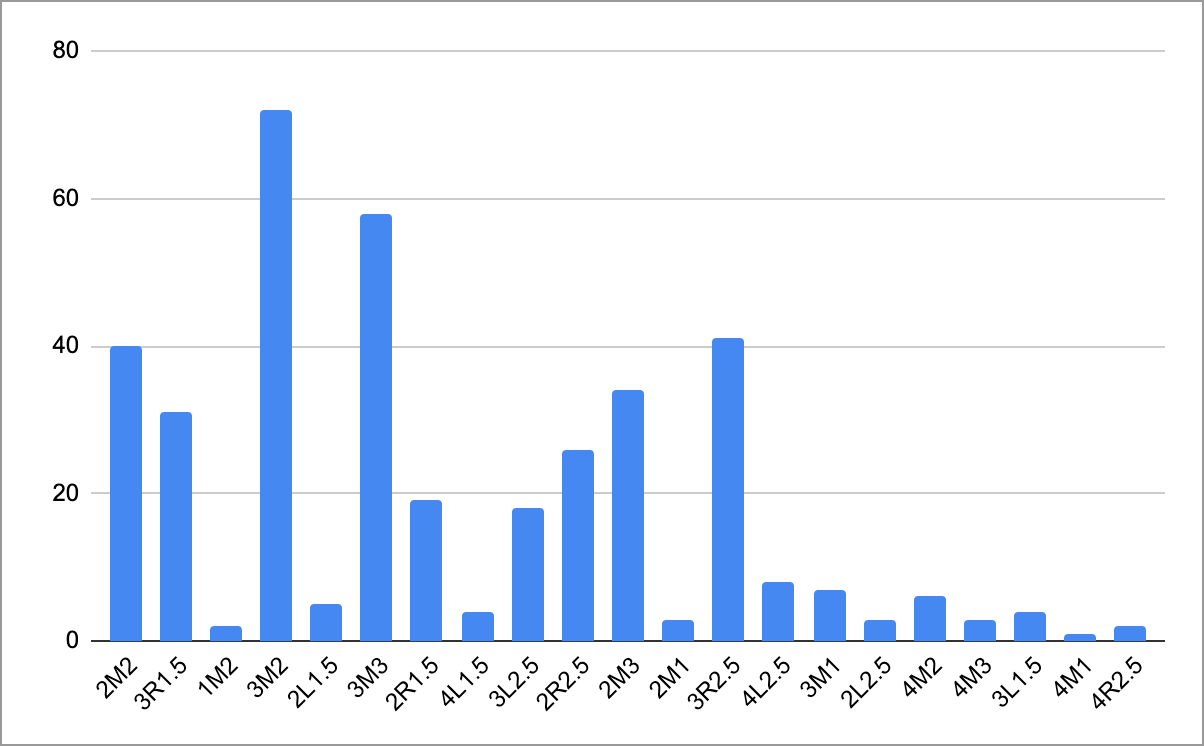
\includegraphics[width=0.9\columnwidth]{pictures/bieu-do-mau-sac-rang.png}
     \caption{Phân bố màu sắc răng hai hàm}
    \label{fig:biểu đồ 3.2}
\end{figure}

\noindent
\textbf{Biểu đồ 3.2.1: Phân bố màu sắc răng hai hàm}\par

\noindent 
\textbf{Nhận xét:}\par
\quad Tỷ lệ màu sắc răng cao nhất ở các đối tượng là màu 3M2, tiếp theo là 3M3 và 3R2.5.\par
\quad Tỷ lệ màu sắc răng thấp nhất là màu 4M1, 4R2.5 và 1M2.



\chapter{BÀN LUẬN}

\textbf{
\section{Đặc điểm màu sắc răng theo bảng màu Vita 3D Master}}

\qquad Biểu đồ 3.1.1 cho thấy tỷ lệ người bệnh nữ cao hơn so với người bệnh nam 2,125 lần.\par
\quad Độ tuổi của đối tượng nghiên cứu từ 20-24 tuổi, là sinh viên trường Đại học Y Dược - Đại học Quốc gia Hà Nội.\par
\quad Bảng 3.1.1 cho thấy tiền sử sử dụng Tetracycline của các đối tượng khá thấp (21,5\% tổng số) và ở nữ nhiều hơn ở nam giới, (nữ: 15,4\% và nam: 6,2\%). Kết quả ở nghiên cứu của Nguyễn Thị Châu \cite{NguyenThiChau} cũng tương tự khi tỷ lệ người bệnh nữ từng sử dụng Tetracycline cao hơn nhiều so với nam. Tình trạng người bệnh 20-24 tuổi có tiền sử sử dụng Tetracycline tương đối thấp so với nhóm tuổi trên 30\cite{NguyenThiChau}.\par
\quad Bảng 3.1.2 cho thấy thói quen sử dụng đồ có màu ở cả hai giới không có sự khác biệt nhiều. Tỷ lệ thói quen sử dụng cocacola là cao nhất (60\%), uống cà phê chiếm 46,2\%, và đồ uống có màu khác chiếm khoảng 44,6\%. Hút thuốc lá chiếm 9,2\% và chỉ gặp ở nam giới, không gặp ở nữ giới. Kết quả này tương đồng với nghiên cứu của Nguyễn Thị Châu\cite{NguyenThiChau}, cho thấy thói quen hút thuốc lá thường gặp ở nam giới. Đặc điểm thói quen sử dụng thực phẩm có màu ảnh hưởng nhiều tới đặc điểm màu sắc răng.\par
\quad Bảng 3.1.3 cho thấy tình trạng vệ sinh răng miệng ở hai giới tương đối đồng đều. Toàn bộ sinh viên vệ sinh răng miệng $\ge$ 2 lần/ngày. Theo báo cáo của Trịnh Thị Tố Quyên\cite{trinhthitoquyen}, 87,8\% đối tượng chải răng hai lần hoặc trên hai lần mỗi ngày và ở báo cáo của Trịnh Minh Báu ở 770 sinh viên, tỷ lệ đánh răng $\ge$ 2 lần/ngày là 90,1\%\cite{trinhminhbau}. Điều này cho thấy ý thức vệ sinh răng miệng hiện nay của sinh viên các trường đại học y đều khá cao và rất tốt.\par
\quad Tỷ lệ sử dụng nước súc miệng có màu sẫm tương đối thấp, khoảng 27,7\%. Tỷ lệ sử dụng nước súc miệng của sinh viên theo Trịnh Minh Báu lại khá cao, 72,2\%.\cite{trinhminhbau}\par
\quad Tình trạng chăm sóc răng miệng định kỳ 6 tháng 1 lần chiếm tỷ lệ khoảng 46,2\%. Tỷ lệ trên 1 năm đi lấy cao răng 1 lần chiếm khoảng 29,2\%. Chưa đi lấy cao răng bao giờ chiếm tỷ lệ 18,5\%. Những con số này cho thấy giới trẻ ngày nay có ý thức cao hơn trong việc chăm sóc vệ sinh răng miệng. Tuy nhiên, thói quen đi kiểm tra định kỳ răng miệng vẫn chưa phổ biến rộng rãi.\par 
\quad Bảng 3.1.4 cho thấy tỷ lệ bề mặt răng nhẵn bóng (92,3\%) cao hơn so với bề mặt răng sần sùi (7,7\%). Đa số các răng không rạn nứt (98,5\%). Không có răng sâu nào. Tỷ lệ tính chất màu sắc răng đồng nhất là 87,7\%, cao hơn tỷ lệ tính chất màu sắc răng không đồng nhất khoảng 7 lần (12,3\%). Ở độ tuổi 20-24, tỷ lệ cao của bề mặt răng nhẵn bóng, răng không bị rạn nứt và không có răng sâu cho thấy tình trạng răng miệng khá tốt. Tuy nhiên, vẫn còn có sự khác biệt về tình trạng răng, nhưng tỷ lệ này không lớn.\par
\quad Hiện nay có nhiều phương pháp đánh giá màu răng: sử dụng bảng so màu bằng băng giấy, sứ có màu hoặc nhựa acrylic, sử dụng phổ quang kế, sắc kế và kỹ thuật phân tích hình ảnh theo Joiner. Nghiên cứu này sử dụng bảng so màu Vita 3D Master.\par
\quad Màu sắc theo bảng Vita 3D Master xác định màu theo phổ màu Munsell: Chroma (độ bão hoà màu), Hue (tông màu), Value (giá trị màu). Phương pháp trực quan này mang tính chủ quan phụ thuộc vào người quan sát và các yếu tố ảnh hưởng tới sự so màu: ánh sáng, thời gian trong ngày, điều kiện thời tiết, môi trường xung quanh, các yếu tố liên quan đến tuổi, kinh nghiệm làm việc, mệt mỏi và trạng thái cảm xúc.\par
\quad Bảng 3.1.5 cho thấy tỷ lệ phân bố giá trị màu sắc răng ở nhóm 3 là cao nhất ở cả 3 nhóm răng (nhóm răng cửa (50,8\%), nhóm răng nanh (53,8\%), nhóm răng hàm nhỏ(53,8\%)) và tương đối ngang nhau giữa hai giới nam và nữ.\par 
\quad Tỷ lệ giá trị màu sắc răng ở nhóm 2 xếp sau với nhóm răng cửa khoảng 43\%, nhóm răng nanh khoảng 40\% và nhóm răng hàm nhỏ khoảng 41,5\%.\par
\quad Nhóm 1 chỉ chiếm tỷ lệ rất nhỏ là 1,5\% và không có đối tượng nào có màu sắc theo nhóm 5.\par
\quad Theo nghiên cứu của Trần Nguyên Lộc\cite{trannguyenloc}, theo bảng màu V3D-M, màu răng có tần suất cao nhất là 2M2 (21,9\%), kế đến là 2M3 (21,1\%). Màu sắc của nhóm nghiên cứu này có tỷ lệ màu răng thuộc nhóm 2 là cao nhất, sự khác biệt kết quả này có thể do rất nhiều nguyên nhân và yếu tố bên ngoài như thói quen sử dụng đồ uống có màu, vệ sinh răng miệng và thói quen khám răng định kỳ.\par 
\quad Bảng 3.1.6 cho thấy tỷ lệ phân bố giá trị màu sắc răng ở nhóm 3 là cao nhất ở cả 3 nhóm răng (nhóm răng cửa (68,8\%), nhóm răng nanh (61\%), nhóm răng hàm nhỏ (70,3\%)) và tương đối ngang nhau giữa hai giới nam và nữ.\par
\quad Tỷ lệ giá trị màu sắc răng ở nhóm 2 xếp sau với nhóm răng cửa khoảng 26,6\%, nhóm răng nanh khoảng 25\% và nhóm răng hàm nhỏ khoảng 25\%.\par
\quad Nhóm 1 và nhóm 5 không có đối tượng nào. \par
\quad Biểu đồ 3.2.2 cho thấy tỷ lệ màu sắc răng cao nhất ở các đối tượng là màu 3M2, tiếp theo là 3M3 và 3R2.5.\par
\quad Tỷ lệ màu sắc răng thấp nhất là màu 4M1,4R2.5 và 1M2.
So sánh với kết quả của Trần Nguyên Lộc\cite{trannguyenloc} thấy được đặc điểm màu sắc răng có sự chênh lệch về màu sắc trên lâm sàng, nguyên nhân có thể đến từ sự khác biệt về độ sáng tối và tông màu, có thể do nguyên nhân ngoại sinh như sử dụng thực phẩm có màu và thói quen vệ sinh răng, tái khám định kỳ là chưa tốt.




\textbf{
\section{Đánh giá nhu cầu làm trắng răng}}
\quad Theo nghiên cứu của Renata Pedrosa Guimarães (2021)\cite{Renata2021}, các nhận thức về những gì là thẩm mỹ hoặc không thẩm mỹ, liên quan đến màu sắc của răng, thay đổi tùy thuộc vào bối cảnh của hiệu suất của mỗi người, bệnh nhân và các chuyên gia. Ý kiến về màu sắc của răng có một cực kỳ tính chất chủ quan và rất khác nhau giữa chuyên gia này và chuyên gia khác. Đa số bệnh nhân tự nhận thấy màu răng của họ tối hơn so với thực tế. Bệnh nhân nữ thường mong muốn có hàm răng sáng màu hơn\cite{LindaGreenwall2019}.\par
\quad Đánh giá nhu cầu làm trắng răng dựa trên 4 yếu tố: sự đổi màu răng, vị trí đổi màu răng, sự ảnh hưởng của màu sắc răng tới cuộc sống người bệnh, và nhu cầu mong muốn làm trắng răng của người bệnh.\par
\quad Bảng 3.2.1 cho thấy sự đổi màu răng ở các đối tượng nghiên cứu là như nhau ở hai giới nam và nữ. Tỷ lệ đổi màu vừa phải cao nhất (90,7\%), tỷ lệ đổi màu nghiêm trọng thấp hơn (4,6\%).\par
\quad Bảng 3.2.2 cho thấy tỷ lệ phân bố vị trí đổi màu răng ở hai giới cũng có sự tương đồng. Phân bố ở ít răng hoặc một răng chiếm tỷ lệ cao nhất (52,3\%). Tỷ lệ phân bố đều ở các răng thấp hơn (40\%). Tỷ lệ phân bố nhiều vết đậm nhạt đồng đều là 3\%. Tỷ lệ phân bố trên các răng phía trước thấp nhất, chiếm 1,5\%.\par
\quad Bảng 3.2.3 cho thấy tỷ lệ của ảnh hưởng màu sắc răng tới người bệnh khiến người bệnh mất tự tin một chút là cao nhất, chiếm khoảng 61,5\%. Tỷ lệ người bệnh không mất tự tin chút nào thấp hơn, khoảng 30,8\%. Tỷ lệ người bệnh hoàn toàn tự tin là rất đẹp và mất tự tin là ngang nhau, khoảng 3\%. \par
\quad Bảng 3.2.5 cho thấy tỷ lệ muốn răng được trắng hơn ở cả nam và nữ đều cao nhất (53,8\%), đặc biệt là nữ (74,3\% trong tổng nữ). Tỷ lệ đối tượng hiện tại đang không quan tâm và đợi làm trắng sau thấp hơn (khoảng 20\%). Tỷ lệ rất muốn được trắng hơn là thấp nhất, chỉ có 3,1\% và đều ở nữ giới.\par
\quad Trong nghiên cứu của Renata Pedrosa Guimarães (2021) về câu hỏi "Bạn có nghĩ rằng bạn cần phải làm trắng răng?"\cite{Renata2021} Tỷ lệ trả lời khẳng định là: nữ cao hơn nhiều so với nam (p=0,001). Các câu trả lời là khẳng định đối với hầu hết sinh viên trong tất cả các khóa học, ngoại trừ những người trong các khóa học y khoa với sự nhấn mạnh về dinh dưỡng học sinh (70,0\%) và học thể dục (63,6\%)\cite{LindaGreenwall2019}.\par
\quad Sự khác biệt giữa hai giới về mong muốn làm trắng răng ở trên cho thấy nữ giới thực sự rất quan tâm tới màu sắc răng và có nhu cầu khá cao về làm trắng răng.\par
\quad Bảng 3.2.4 cho thấy tỷ lệ nhu cầu làm trắng răng mức trung bình là cao nhất ở cả hai giới nam và nữ, chiếm khoảng 66,2\%. Tỷ lệ nhu cầu làm trắng răng mức mong muốn thấp hơn, chiếm 18,5\%. Tỷ lệ nhu cầu làm trắng răng mức khuyến cáo là 7,7\%, mức có thể là 4,6\% và ở mức cao là 3\%.\par
\quad Có thể nhấn mạnh rằng: hơn một nửa (53,9\%) câu trả lời là tẩy trắng răng; có một mối liên quan đáng kể giữa chỉ định của làm trắng với chuyên ngành và thời gian kể từ khi ra trường. Tỷ lệ các dấu hiệu tích cực cao hơn trong số bác sỹ thuộc các chuyên khoa: Răng Hàm Mặt, Răng Hàm Mặt + Chỉnh Nha và Răng Hàm Mặt + Cấy Ghép Implant, và thấp hơn giữa các chuyên khoa Răng Hàm Mặt + Nội Nha, Nội Nha, Nhi Khoa và Nha Chu. Cao nhất phần trăm phản hồi có chỉ định tẩy trắng xảy ra ở những người có hơn 20 năm tốt nghiệp (65,3\%) và thấp nhất là nhóm từ 10 đến 19 tuổi (35,6\%)\cite{LindaGreenwall2019}.\par
\quad Từ những kết quả trên, có thể nhận thấy rằng nhu cầu làm trắng răng được đánh giá dựa trên nhiều yếu tố để có thể đưa ra được kết luận phù hợp, đồng thời hài lòng cả bác sĩ và người bệnh.\par
\quad Bảng 3.2.6 cho thấy tỷ lệ màu sắc mong muốn của người bệnh ở màu 1M1 ở nữ là cao nhất, chiếm 36,4\% tổng số. Tỷ lệ màu sắc mong muốn của nữ giới ở màu 0M3 và 1M2 là như nhau (13,6\%). Tỷ lệ màu sắc mong muốn của nam giới ở màu 2M1 và 1M2 là cao nhất (7.7\%). Tỷ lệ màu sắc mong muốn ở nhóm 0 ở nữ giới cao hơn nam giới (ở nữ: 29,5\%; ở nam: 19\%).\par
\quad Từ đó, có thể thấy rằng nhu cầu làm trắng răng theo đánh giá của bác sĩ và mong muốn của người bệnh có một sự liên quan mật thiết, với nhu cầu thẩm mỹ của nữ giới là rất cao. Tuy nhiên bên cạnh đó có thể thấy được hiện nay nam giới cũng có nhu cầu nhất định liên quan đến thẩm mỹ.



\chapter*{KẾT LUẬN}

\vspace{5pt}
\qquad Từ kết quả nghiên cứu đặc điểm màu sắc răng theo bảng màu Vita 3D Master và đánh giá nhu cầu làm trắng răng của người bệnh chúng tôi rút ra các kết luận sau:\par

\textbf{
\section*{1. Xác định đặc điểm màu sắc răng theo bảng màu Vita 3D Master}}
\quad Trong 65 người bệnh lựa chọn ngẫu nhiên, tỷ lệ nữ cao hơn nam khoảng hơn 2 lần. Độ tuổi của đối tượng nghiên cứu là 20-24 tuổi.\par
\quad Màu sắc răng: nhóm 1, nhóm 2 và nhóm 3 ở hàm trên và nhóm 2, nhóm 3 và nhóm 4 ở hàm dưới. \par 
\quad Tỷ lệ phân bố giá trị màu sắc răng hàm trên ở nhóm 3 là cao nhất ở cả 3 nhóm răng (nhóm răng cửa (50,8\%), nhóm răng nanh (53,8\%), nhóm răng hàm nhỏ(53,8\%)). Tỷ lệ màu sắc răng ở nhóm 2 xếp sau với nhóm răng cửa khoảng 43\%, nhóm răng nanh khoảng 40\% và nhóm răng hàm nhỏ khoảng 41,5\%. Nhóm 1 chỉ chiếm tỷ lệ rất nhỏ là 1,5\% và không có đối tượng nào có màu sắc theo nhóm 5.\par
\quad Tỷ lệ phân bố giá trị màu sắc răng hàm dưới ở nhóm 3 là cao nhất ở cả 3 nhóm răng (nhóm răng cửa (68,8\%), nhóm răng nanh (61\%), nhóm răng hàm nhỏ (70,3\%)). Tỷ lệ màu sắc răng ở nhóm 2 xếp sau với nhóm răng cửa khoảng 26,6\%, nhóm răng nanh khoảng 25\% và nhóm răng hàm nhỏ khoảng 25\%. Nhóm 1 và nhóm 5 không có đối tượng nào.\par
\quad Tỷ lệ màu sắc răng cao nhất ở các đối tượng là màu 3M2, tiếp theo là 3M3 và 3R2.5. Tỷ lệ màu sắc răng thấp nhất là màu 4M1,4R2.5 và 1M2.\par 
\quad Màu sắc răng giữa các nhóm răng cửa, răng nanh và hàm nhỏ là không đồng nhất, màu đậm nhất là nhóm răng nanh. Đa số màu sắc răng ở màu trung tính, một số răng có độ đỏ và độ vàng, chủ yếu ở nhóm răng nanh.\par 
\quad Bề mặt răng đa số nhẵn bóng, không nứt, có tính chất đồng nhất và không sâu răng. 
\vspace{-5pt}
\textbf{
\section*{2. Đánh giá nhu cầu làm trắng răng ở sinh viên trường Đại học Y Dược}}
\quad Tỷ lệ của ảnh hưởng màu sắc răng tới người bệnh khiến người bệnh mất tự tin một chút là cao nhất, chiếm khoảng 61,5\%. Tỷ lệ người bệnh không mất tự tin chút nào thấp hơn, khoảng 30,8\%. Tỷ lệ người bệnh hoàn toàn tự tin là rất đẹp và mất tự tin là ngang nhau, khoảng 3\%.\par
\quad Tỷ lệ muốn răng được trắng hơn ở cả nam và nữ đều cao nhất (53,8\%), đặc biệt là nữ (74,3\% trong tổng nữ). Tỷ lệ đối tượng hiện tại đang không quan tâm và đợi làm trắng sau thấp hơn (khoảng 20\%). Tỷ lệ rất muốn được trắng hơn là thấp nhất, chỉ có 3,1\% và đều ở nữ giới.\par
\quad Tỷ lệ nhu cầu làm trắng răng mức trung bình là cao nhất ở cả hai giới nam và nữ, chiếm khoảng 66,2\%. Tỷ lệ nhu cầu làm trắng răng mức mong muốn thấp hơn, chiếm 18,5\%. Tỷ lệ nhu cầu làm trắng răng mức khuyến cáo là 7,7\%, mức có thể là 4,6\% và ở mức cao là 3\%.\par
\quad Tỷ lệ màu sắc mong muốn của người bệnh ở màu 1M1 ở nữ là cao nhất, chiếm 36,4\% tổng số. Tỷ lệ màu sắc mong muốn của nữ giới ở màu 0M3 và 1M2 là như nhau (13,6\%). Tỷ lệ màu sắc mong muốn của nam giới ở màu 2M1 và 1M2 là cao nhất (7.7\%). Tỷ lệ màu sắc mong muốn ở nhóm 0 ở nữ giới cao hơn nam giới (ở nữ: 29,5\%; ở nam: 19\%).


\chapter*{KIẾN NGHỊ}
\vspace{5pt}
\qquad Từ kết quả trên, chúng tôi đưa ra một số kiến nghị sau:\par 
\begin{itemize}
\setlength{\itemsep}{0pt}
    \item Chỉ số nhu cầu điều trị làm trắng răng nên được phát triển hơn và có thể đưa ra thang điểm đánh giá cụ thể hoá các yếu tố đánh giá hơn để đánh giá tốt hơn về nhu cầu làm trắng răng.
    \item Tuy tỷ lệ người bệnh có thói quen vệ sinh răng miệng tốt là rất cao, tỷ lệ người bệnh đi khám định kỳ thường xuyên 3-6 tháng 1 lần không quá thấp, nhưng thói quen đi kiểm tra răng miệng định kỳ nên phổ biến rộng rãi hơn để người bệnh có thể có ý thức chăm sóc răng miệng được tốt hơn để có thể đạt được kết quả tốt nhất về thẩm mỹ cũng như sức khoẻ của răng miệng. 
    \item Đánh giá đặc điểm màu sắc răng nên được sử dụng các phương pháp đánh giá màu khách quan hơn bằng cách sử dụng các thiết kế đo màu hiện đại, tuy nhiên, phương pháp này khá tốn kém nên chưa quá phổ biến ở các phòng khám hiện tại.
\end{itemize}



\addcontentsline{toc}{chapter}{KẾT LUẬN}
\addcontentsline{toc}{chapter}{KIẾN NGHỊ}
\singlespacing

\clearpage
\renewcommand{\thepage}{}
\bibliography{refs}
\addcontentsline{toc}{chapter}{TÀI LIỆU THAM KHẢO}
\bibliographystyle{plainnat}

\newpage
\begin{appendices}
\addtocontents{toc}{\protect\setcounter{tocdepth}{-1}}
\addcontentsline{toc}{chapter}{PHỤ LỤC}
\chapter*{PHỤ LỤC}
\newpage
\begin{center}
    \textbf{BẢN CUNG CẤP THÔNG TIN NGHIÊN CỨU VÀ PHIẾU TÌNH NGUYỆN THAM GIA NGHIÊN CỨU}\par
\end{center}

\noindent
\textbf{Tên nghiên cứu: “Đặc điểm màu răng theo bảng màu Vita 3D và xác định nhu cầu làm trắng răng ở sinh viên trường Đại học Y Dược - Đại học Quốc gia Hà Nội”}\\
\vspace{3pt}
\textbf{Nghiên cứu viên chính:} Nguyễn Thu Trà – SV năm 6 lớp Răng Hàm Mặt – Trường Đại học Y Dược – Đại học Quốc gia Hà Nội\\
\vspace{3pt}
\noindent
\textbf{Mục đích và cách tiến hành nghiên cứu}
\begin{itemize}
\setlength{\itemsep}{0pt}
    \item Mục đích của nghiên cứu:
    \begin{itemize}
    \setlength{\itemsep}{0pt}
        \item Xác định đặc điểm màu răng theo bảng Vita 3D ở sinh viên trường Đại học Y Dược - Đại học Quốc Gia Hà Nội.
        \item Xác định nhu cầu làm trắng răng ở đối tượng trên.
    \end{itemize}
    \item Tiêu chuẩn lựa chọn đối tượng:
    \begin{itemize}
    \setlength{\itemsep}{0pt}
        \item Sinh viên trường Đại học Y Dược - Đại học Quốc Gia Hà Nội.
        \item Người bệnh tự nguyện tham gia nghiên cứu.
    \end{itemize}
    \item Tiêu chuẩn loại trừ khỏi nghiên cứu:
    \begin{itemize}
    \setlength{\itemsep}{0pt}
        \item Không đáp ứng các tiêu chuẩn lựa chọn.
        \item Người bệnh đang chỉnh nha.
        \item Người bệnh đã làm phục hình răng.
    \end{itemize}
    \item Chúng tôi mời anh/chị tham gia trả lời thông tin cá nhân, một số câu hỏi khảo sát và được thăm khám trên ghế răng.
\end{itemize}

\noindent
\textbf{Quyền lợi của đối tượng}\par
\vspace{3pt}
\quad Những thông tin mà anh/chị cung cấp cho chúng tôi, sẽ giúp chúng tôi đưa ra những khuyến nghị/giải pháp phù hợp với bản thân của anh/chị.\\
\vspace{4pt}
\textbf{Các nguy cơ và bất lợi}\par
\vspace{2pt}
\quad Chúng tôi tiến hành phỏng vấn và không có bất kì can thiệp nào nên anh/chị hầu như không có nguy hại gì tới sức khỏe khi tham gia nghiên cứu.\\
\vspace{4pt}
\textbf{Bảo mật thông tin}\par
\vspace{2pt}
\quad Mọi thông tin anh/chị cung cấp cho nghiên cứu đều được bảo mật và chỉ phục vụ mục đích nghiên cứu. Thông tin cá nhân của anh/chị đều được mã hóa trước khi xử lý số liệu và tiến hành phân tích. Chỉ có nghiên cứu viên chính mới có quyền tiếp cận thông tin của anh/chị.\\
\vspace{4pt}
\textbf{Bồi thường hoặc chăm sóc, điều trị nếu có biến cố về sức khỏe xảy ra liên quan đến nghiên cứu}\par
\vspace{2pt}
\quad Trong trường hợp xảy ra chấn thương hoặc tổn thương do việc tham gia vào nghiên cứu gây ra, anh/chị tham gia nghiên cứu sẽ được điều trị miễn phí.


\newpage
\begin{center}
\textbf{PHIẾU CHẤP THUẬN THAM GIA NGHIÊN CỨU}\par
\end{center}
\textbf{Tên đề tài nghiên cứu: “Đặc điểm màu răng theo bảng màu Vita 3D và xác định nhu cầu làm trắng răng ở sinh viên trường Đại học Y Dược - Đại học Quốc gia Hà Nội”}\par
\quad Đây là nghiên cứu khoa học nhằm mục tiêu xác định đặc điểm màu răng và nhu cầu làm trắng răng ở sinh viên trường Đại học Y Dược - Đại học Quốc Gia Hà Nội năm 2023. Khi ký vào đơn đồng ý, anh/chị sẽ tham gia vào một phỏng vấn.\par
\quad Mọi thông tin trong nghiên cứu đều được giữ bí mật và chỉ phục vụ cho mục đích nghiên cứu. Việc tham gia phỏng vấn và thăm khám của anh/chị là hoàn toàn tự nguyện. Nếu muốn anh/chị có thể từ chối không không trả lời các câu hỏi phỏng vấn và dừng việc thăm khám vào bất cứ lúc nào. Anh/chị sẽ không phải trả bất kỳ một khoản lệ phí nào cho nghiên cứu này.\\
\textbf{XÁC NHẬN ĐỒNG Ý TRẢ LỜI PHỎNG VẤN}\\
Tôi tên:.......................................................................................
\begin{enumerate}
\setlength{\itemsep}{0pt}
    \item Tôi xác nhận rằng đã nhận được thông tin về nghiên cứu này. Tôi cũng có cơ hội để đặt câu hỏi và tôi hoàn toàn đồng ý với thông tin được cung cấp. 
    \item Tôi hiểu rằng việc tham gia của tôi là tự nguyện và miễn phí. Tôi có quyền rút lui khỏi nghiên cứu bất cứ lúc nào mà không cần đưa ra lý do. Điều này không hề ảnh hưởng đến các quyền lợi chăm sóc y tế về sau.
    \item Tôi đồng ý tham gia nghiên cứu đã nêu trên.
\end{enumerate}

Ngày\hspace{1cm}tháng\hspace{1cm}năm 2023\par
Người tham gia nghiên cứu\hspace{5cm}Nghiên cứu viên\par
\hspace{1cm}(Ký, ghi rõ họ tên)	\hspace{5cm}(Ký, ghi rõ họ tên)



\chapter*{PHỤ LỤC 1: BỘ CÂU HỎI KHẢO SÁT}
\vspace{5pt}
\begin{flushright}
    \textbf{Mã số:}\hspace{2cm} \par
\end{flushright}
\vspace{12pt}
\section*{Thông tin cá nhân}

\begin{itemize}
    \item Họ và tên:
    \item Tuổi:
    \item Giới tính: Nam/Nữ
    \item Lớp:
    \item Địa chỉ: 
    \item Liên hệ:
\end{itemize}
\vspace{12pt}
\section*{Câu hỏi}

\textbf{Bạn có tự tin vào màu sắc hàm răng của mình không?}
\begin{enumerate}
    \item Rất mất tự tin
    \item Mất tự tin
    \item Mất tự tin một chút
    \item Không mất tự tin chút nào
    \item Hoàn toàn tự tin là rất đẹp
\end{enumerate}

\noindent
\textbf{Bạn muốn hàm răng mình được trắng hơn đến mức nào?}
\begin{enumerate}
    \item Rất muốn được trắng hơn
    \item Muốn răng được trắng hơn
    \item Thấy răng có nhiễm màu và muốn các răng đó sáng hơn
    \item Nếu những răng nhiễm màu sáng hơn thì tốt
    \item Thấy có răng nhiễm màu nhưng không quan tâm, đợi làm trắng răng sau
\end{enumerate}
  
\noindent
\textbf{Bạn có tiền sử sử dụng kháng sinh Tetracycline không?}
\par
\vspace{5pt}
\begin{enumerate*}[start=0, itemjoin={\hspace{5cm}}]
    \setcounter{enumi}{-1}
    \item Không
    \item Có
\end{enumerate*}
\vspace{5pt}
\par
\noindent
\textbf{Bạn có tiền sử bị chấn thương răng không?}
\par
\vspace{5pt}
\begin{enumerate*}[start=0, itemjoin={\hspace{5cm}}]
    \setcounter{enumi}{-1}
    \item Không
    \item Có
\end{enumerate*}
\vspace{5pt}
\par
\noindent
\textbf{Bạn đã từng sử dụng thuốc tẩy trắng chưa?}
\par
\vspace{5pt}
\begin{enumerate*}[start=0, itemjoin={\hspace{5cm}}]
    \setcounter{enumi}{-1}
    \item Không
    \item Có
\end{enumerate*}
\vspace{5pt}
\par
\noindent
\textbf{Bạn có đã hoặc đang hút thuốc lá không?}
\par
\vspace{5pt}
\begin{enumerate*}[start=0, itemjoin={\hspace{5cm}}]
    \setcounter{enumi}{-1}
    \item Không
    \item Có
\end{enumerate*}
\vspace{5pt}
\par
\noindent
\textbf{Bạn hiện tại có đang sử dụng đồ uống có màu không?}
\begin{itemize}
    \item Cafe:
    \begin{enumerate*}
        \setcounter{enumi}{-1}
        \item Không
        \item Có
    \end{enumerate*}
    \item Nước chè:
    \begin{enumerate*}[start=0]
        \item Không
        \item Có
    \end{enumerate*}
    \item Coca cola:
    \begin{enumerate*}[start=0]
        \item Không
        \item Có
    \end{enumerate*}
    \item Các loại đồ uống có màu sẫm khác:
    \begin{enumerate*}[start=0]
        \item Không
        \item Có
    \end{enumerate*}
\end{itemize}

\par
\noindent
\textbf{Bạn vệ sinh răng miệng bao nhiêu lần trong ngày?}
\par
\vspace{5pt}
\begin{enumerate*}[start=0, itemjoin={\hspace{3cm}}]
    \setcounter{enumi}{-1}
    \item 1 lần/ngày
    \item 2 lần/ngày
    \item trên 2 lần/ngày
\end{enumerate*}
\vspace{5pt}
\par
\noindent
\textbf{Bạn có sử dụng nước súc miệng có màu sẫm sau khi vệ sinh răng không?}
\par
\vspace{5pt}
\begin{enumerate*}[start=0, itemjoin={\hspace{5cm}}]
    \setcounter{enumi}{-1}
    \item Không
    \item Có
\end{enumerate*}
\vspace{5pt}
\par
\noindent
\textbf{Bạn có thường xuyên đi lấy cao răng định kỳ không?}
\begin{enumerate}[start=0, itemjoin={\hspace{5cm}}]
    \setcounter{enumi}{-1}
    \item Chưa bao giờ lấy cao răng
    \item Lấy cao răng 3 tháng 1 lần
    \item Lấy cao răng 6 tháng 1 lần
    \item Trên 1 năm đi lấy cao răng 1 lần 
\end{enumerate}

\par
\noindent
\textbf{Bạn mong muốn làm trắng răng đến màu sắc nào? (kèm bảng màu Vita)}
\begin{enumerate}[start=0]
    \setcounter{enumi}{-1}
    \item Màu khác
    \item 2M3
    \item 2M2
    \item 2M1
    \item 1M2
    \item 1M1
    \item 0M3
    \item 0M2
    \item 0M1
\end{enumerate}

\chapter*{PHỤ LỤC 2: PHIẾU KHÁM RĂNG}
\vspace{5pt}
\begin{flushright}
    \textbf{Mã số:}\hspace{2cm} \par
\end{flushright}
\vspace{-0pt}
\textbf{Ngày khám:} \par
\noindent
\rule{\linewidth}{0.4pt}

\vspace{0.9pt}
\par
\noindent
\textbf{Bề mặt răng}
\par
\vspace{5pt}
\begin{enumerate*}[start=0, itemjoin={\hspace{4cm}}]
    \setcounter{enumi}{-1}
    \item Nhẵn bóng
    \item Sần sùi
\end{enumerate*}
\vspace{5pt}

\par
\noindent
\textbf{Răng rạn nứt}
\par
\vspace{5pt}
\begin{enumerate*}[start=0, itemjoin={\hspace{5cm}}]
    \setcounter{enumi}{-1}
    \item Không
    \item Có
\end{enumerate*}
\vspace{5pt}

\par
\noindent
\textbf{Răng bị sâu}
\par
\vspace{5pt}
\begin{enumerate*}[start=0, itemjoin={\hspace{5cm}}]
    \setcounter{enumi}{-1}
    \item Không
    \item Có
\end{enumerate*}
\vspace{5pt}

\par
\noindent
\textbf{Tính chất màu sắc răng}
\par
\vspace{5pt}
\begin{enumerate*}[start=0, itemjoin={\hspace{3cm}}]
    \setcounter{enumi}{-1}
    \item Không đồng nhất
    \item Đồng nhất
\end{enumerate*}
\vspace{5pt}

\par
\noindent
\textbf{Sự đổi màu răng}
\begin{enumerate}[start=0, itemjoin={\hspace{5cm}}]
 \setlength{\itemsep}{0pt}
    \setcounter{enumi}{-1}
    \item Đổi màu nghiêm trọng
    \item Đổi màu vừa phải
    \item Đổi màu nhẹ
    \item Đổi màu nhẹ hoặc đốm trắng
\end{enumerate}


\par
\noindent
\textbf{Vị trí đổi màu}
\begin{enumerate}[start=0, itemjoin={\hspace{5cm}}]
\setlength{\itemsep}{0pt}
    \setcounter{enumi}{-1}
    \item Phân bố nhiều vết đậm nhạt đồng đều
    \item Phân bố đều các răng
    \item Phân bố trên các răng phía trước
    \item Phân bố ngẫu nhiên trên răng
    \item Phân bố ở ít răng hoặc một răng
\end{enumerate}


\par
\noindent
\textbf{Màu sắc răng}
\par

\begin{longtblr}[
    caption = {Màu sắc răng}, 
    entry = none,
]{
  column{2} = {c},
  cell{1}{1} = {c=2}{},
  cell{1}{3} = {c},
  cell{1}{4} = {c},
  cell{1}{5} = {c},
  cell{1}{6} = {c},
  cell{1}{7} = {c},
  cell{1}{8} = {c},
  cell{1}{9} = {c},
  cell{1}{10} = {c},
  cell{1}{11} = {c},
  cell{1}{12} = {c},
  cell{2}{1} = {r=3}{c},
  cell{5}{1} = {r=2}{c},
  cell{7}{1} = {r=3}{},
  cell{10}{1} = {c},
  cell{11}{1} = {r=3}{},
  cell{14}{1} = {r=7}{c},
  cell{21}{1} = {r=7}{c},
  cell{28}{1} = {r=3}{c},
  cell{30}{12} = {c},
  vlines,
  hline{1-2,5,7,14,21,28,31} = {-}{},
  hline{3-4,6,8-13,15-20,22-27,29-30} = {2-12}{},
}
       &       & R15 & R14 & R13 & R12 & R11 & R21 & R22 & R23 & R24 & R25 \\
Nhóm 0 & 0M1   &     &     &     &     &     &     &     &     &     &     \\
       & 0M2   &     &     &     &     &     &     &     &     &     &     \\
       & 0M3   &     &     &     &     &     &     &     &     &     &     \\
Nhóm 1 & 1M1   &     &     &     &     &     &     &     &     &     &     \\
       & 1M2   &     &     &     &     &     &     &     &     &     &     \\
       & 2L1.5 &     &     &     &     &     &     &     &     &     &     \\
       & 2L2.5 &     &     &     &     &     &     &     &     &     &     \\
       & 2M1   &     &     &     &     &     &     &     &     &     &     \\
Nhóm 2 & 2M2   &     &     &     &     &     &     &     &     &     &     \\
       & 2M3   &     &     &     &     &     &     &     &     &     &     \\
       & 2R1.5 &     &     &     &     &     &     &     &     &     &     \\
       & 2R2.5 &     &     &     &     &     &     &     &     &     &     \\
Nhóm 3 & 3L1.5 &     &     &     &     &     &     &     &     &     &     \\
       & 3L2.5 &     &     &     &     &     &     &     &     &     &     \\
       & 3M1   &     &     &     &     &     &     &     &     &     &     \\
       & 3M2   &     &     &     &     &     &     &     &     &     &     \\
       & 3M3   &     &     &     &     &     &     &     &     &     &     \\
       & 3R1.5 &     &     &     &     &     &     &     &     &     &     \\
       & 3R2.5 &     &     &     &     &     &     &     &     &     &     \\
Nhóm 4 & 4L1.5 &     &     &     &     &     &     &     &     &     &     \\
       & 4L2.5 &     &     &     &     &     &     &     &     &     &     \\
       & 4M1   &     &     &     &     &     &     &     &     &     &     \\
       & 4M2   &     &     &     &     &     &     &     &     &     &     \\
       & 4M3   &     &     &     &     &     &     &     &     &     &     \\
       & 4R1.5 &     &     &     &     &     &     &     &     &     &     \\
       & 4R2.5 &     &     &     &     &     &     &     &     &     &     \\
Nhóm 5 & 5M1   &     &     &     &     &     &     &     &     &     &     \\
       & 5M2   &     &     &     &     &     &     &     &     &     &     \\
       & 5M3   &     &     &     &     &     &     &     &     &     &     
\end{longtblr}

\begin{longtblr}[
    entry = none,
]{
  column{2} = {c},
  cell{1}{1} = {c=2}{},
  cell{1}{3} = {c},
  cell{1}{4} = {c},
  cell{1}{5} = {c},
  cell{1}{6} = {c},
  cell{1}{7} = {c},
  cell{1}{8} = {c},
  cell{1}{9} = {c},
  cell{1}{10} = {c},
  cell{1}{11} = {c},
  cell{1}{12} = {c},
  cell{2}{1} = {r=3}{c},
  cell{5}{1} = {r=2}{c},
  cell{7}{1} = {r=3}{},
  cell{10}{1} = {c},
  cell{11}{1} = {r=3}{},
  cell{14}{1} = {r=7}{c},
  cell{21}{1} = {r=7}{c},
  cell{28}{1} = {r=3}{c},
  cell{30}{12} = {c},
  vlines,
  hline{1-2,5,7,14,21,28,31} = {-}{},
  hline{3-4,6,8-13,15-20,22-27,29-30} = {2-12}{},
}
       &       & R45 & R44 & R43 & R42 & R41 & R31 & R32 & R33 & R34 & R35 \\
Nhóm 0 & 0M1   &     &     &     &     &     &     &     &     &     &     \\
       & 0M2   &     &     &     &     &     &     &     &     &     &     \\
       & 0M3   &     &     &     &     &     &     &     &     &     &     \\
Nhóm 1 & 1M1   &     &     &     &     &     &     &     &     &     &     \\
       & 1M2   &     &     &     &     &     &     &     &     &     &     \\
       & 2L1.5 &     &     &     &     &     &     &     &     &     &     \\
       & 2L2.5 &     &     &     &     &     &     &     &     &     &     \\
       & 2M1   &     &     &     &     &     &     &     &     &     &     \\
Nhóm 2 & 2M2   &     &     &     &     &     &     &     &     &     &     \\
       & 2M3   &     &     &     &     &     &     &     &     &     &     \\
       & 2R1.5 &     &     &     &     &     &     &     &     &     &     \\
       & 2R2.5 &     &     &     &     &     &     &     &     &     &     \\
Nhóm 3 & 3L1.5 &     &     &     &     &     &     &     &     &     &     \\
       & 3L2.5 &     &     &     &     &     &     &     &     &     &     \\
       & 3M1   &     &     &     &     &     &     &     &     &     &     \\
       & 3M2   &     &     &     &     &     &     &     &     &     &     \\
       & 3M3   &     &     &     &     &     &     &     &     &     &     \\
       & 3R1.5 &     &     &     &     &     &     &     &     &     &     \\
       & 3R2.5 &     &     &     &     &     &     &     &     &     &     \\
Nhóm 4 & 4L1.5 &     &     &     &     &     &     &     &     &     &     \\
       & 4L2.5 &     &     &     &     &     &     &     &     &     &     \\
       & 4M1   &     &     &     &     &     &     &     &     &     &     \\
       & 4M2   &     &     &     &     &     &     &     &     &     &     \\
       & 4M3   &     &     &     &     &     &     &     &     &     &     \\
       & 4R1.5 &     &     &     &     &     &     &     &     &     &     \\
       & 4R2.5 &     &     &     &     &     &     &     &     &     &     \\
Nhóm 5 & 5M1   &     &     &     &     &     &     &     &     &     &     \\
       & 5M2   &     &     &     &     &     &     &     &     &     &     \\
       & 5M3   &     &     &     &     &     &     &     &     &     &     
\end{longtblr}


\chapter*{DANH SÁCH SINH VIÊN THAM GIA NGHIÊN CỨU}

\begin{longtblr}[
    entry=none
]{
  width = \linewidth,
  colspec = {Q[85]Q[296]Q[63]Q[119]Q[102]Q[269]},
  row{1} = {c},
  cell{2}{1} = {c},
  cell{2}{3} = {c},
  cell{2}{4} = {c},
  cell{3}{1} = {c},
  cell{3}{3} = {c},
  cell{3}{4} = {c},
  cell{4}{1} = {c},
  cell{4}{3} = {c},
  cell{4}{4} = {c},
  cell{5}{1} = {c},
  cell{5}{3} = {c},
  cell{5}{4} = {c},
  cell{6}{1} = {c},
  cell{6}{3} = {c},
  cell{6}{4} = {c},
  cell{7}{1} = {c},
  cell{7}{3} = {c},
  cell{7}{4} = {c},
  cell{8}{1} = {c},
  cell{8}{3} = {c},
  cell{8}{4} = {c},
  cell{9}{1} = {c},
  cell{9}{3} = {c},
  cell{9}{4} = {c},
  cell{10}{1} = {c},
  cell{10}{3} = {c},
  cell{10}{4} = {c},
  cell{11}{1} = {c},
  cell{11}{3} = {c},
  cell{11}{4} = {c},
  cell{12}{1} = {c},
  cell{12}{3} = {c},
  cell{12}{4} = {c},
  cell{13}{1} = {c},
  cell{13}{3} = {c},
  cell{13}{4} = {c},
  cell{14}{1} = {c},
  cell{14}{3} = {c},
  cell{14}{4} = {c},
  cell{15}{1} = {c},
  cell{15}{3} = {c},
  cell{15}{4} = {c},
  cell{16}{1} = {c},
  cell{16}{3} = {c},
  cell{16}{4} = {c},
  cell{17}{1} = {c},
  cell{17}{3} = {c},
  cell{17}{4} = {c},
  cell{18}{1} = {c},
  cell{18}{3} = {c},
  cell{18}{4} = {c},
  cell{19}{1} = {c},
  cell{19}{3} = {c},
  cell{19}{4} = {c},
  cell{20}{1} = {c},
  cell{20}{3} = {c},
  cell{20}{4} = {c},
  cell{21}{1} = {c},
  cell{21}{3} = {c},
  cell{21}{4} = {c},
  cell{22}{1} = {c},
  cell{22}{3} = {c},
  cell{22}{4} = {c},
  cell{23}{1} = {c},
  cell{23}{3} = {c},
  cell{23}{4} = {c},
  cell{24}{1} = {c},
  cell{24}{3} = {c},
  cell{24}{4} = {c},
  cell{25}{1} = {c},
  cell{25}{3} = {c},
  cell{25}{4} = {c},
  cell{26}{1} = {c},
  cell{26}{3} = {c},
  cell{26}{4} = {c},
  cell{27}{1} = {c},
  cell{27}{3} = {c},
  cell{27}{4} = {c},
  cell{28}{1} = {c},
  cell{28}{3} = {c},
  cell{28}{4} = {c},
  cell{29}{1} = {c},
  cell{29}{3} = {c},
  cell{29}{4} = {c},
  cell{30}{1} = {c},
  cell{30}{3} = {c},
  cell{30}{4} = {c},
  cell{31}{1} = {c},
  cell{31}{3} = {c},
  cell{31}{4} = {c},
  cell{32}{1} = {c},
  cell{32}{3} = {c},
  cell{32}{4} = {c},
  cell{33}{1} = {c},
  cell{33}{3} = {c},
  cell{33}{4} = {c},
  cell{34}{1} = {c},
  cell{34}{3} = {c},
  cell{34}{4} = {c},
  cell{35}{1} = {c},
  cell{35}{3} = {c},
  cell{35}{4} = {c},
  cell{36}{1} = {c},
  cell{36}{3} = {c},
  cell{36}{4} = {c},
  cell{37}{1} = {c},
  cell{37}{3} = {c},
  cell{37}{4} = {c},
  cell{38}{1} = {c},
  cell{38}{3} = {c},
  cell{38}{4} = {c},
  cell{39}{1} = {c},
  cell{39}{3} = {c},
  cell{39}{4} = {c},
  cell{40}{1} = {c},
  cell{40}{3} = {c},
  cell{40}{4} = {c},
  cell{41}{1} = {c},
  cell{41}{3} = {c},
  cell{41}{4} = {c},
  cell{42}{1} = {c},
  cell{42}{3} = {c},
  cell{42}{4} = {c},
  cell{43}{1} = {c},
  cell{43}{3} = {c},
  cell{43}{4} = {c},
  cell{44}{1} = {c},
  cell{44}{3} = {c},
  cell{44}{4} = {c},
  cell{45}{1} = {c},
  cell{45}{3} = {c},
  cell{45}{4} = {c},
  cell{46}{1} = {c},
  cell{46}{3} = {c},
  cell{46}{4} = {c},
  cell{47}{1} = {c},
  cell{47}{3} = {c},
  cell{47}{4} = {c},
  cell{48}{1} = {c},
  cell{48}{3} = {c},
  cell{48}{4} = {c},
  cell{49}{1} = {c},
  cell{49}{3} = {c},
  cell{49}{4} = {c},
  cell{50}{1} = {c},
  cell{50}{3} = {c},
  cell{50}{4} = {c},
  cell{51}{1} = {c},
  cell{51}{3} = {c},
  cell{51}{4} = {c},
  cell{52}{1} = {c},
  cell{52}{3} = {c},
  cell{52}{4} = {c},
  cell{53}{1} = {c},
  cell{53}{3} = {c},
  cell{53}{4} = {c},
  cell{54}{1} = {c},
  cell{54}{3} = {c},
  cell{54}{4} = {c},
  cell{55}{1} = {c},
  cell{55}{3} = {c},
  cell{55}{4} = {c},
  cell{56}{1} = {c},
  cell{56}{3} = {c},
  cell{56}{4} = {c},
  cell{57}{1} = {c},
  cell{57}{3} = {c},
  cell{57}{4} = {c},
  cell{58}{1} = {c},
  cell{58}{3} = {c},
  cell{58}{4} = {c},
  cell{59}{1} = {c},
  cell{59}{3} = {c},
  cell{59}{4} = {c},
  cell{60}{1} = {c},
  cell{60}{3} = {c},
  cell{60}{4} = {c},
  cell{61}{1} = {c},
  cell{61}{3} = {c},
  cell{61}{4} = {c},
  cell{62}{1} = {c},
  cell{62}{3} = {c},
  cell{62}{4} = {c},
  cell{63}{1} = {c},
  cell{63}{3} = {c},
  cell{63}{4} = {c},
  cell{64}{1} = {c},
  cell{64}{3} = {c},
  cell{64}{4} = {c},
  cell{65}{1} = {c},
  cell{65}{3} = {c},
  cell{65}{4} = {c},
  cell{66}{1} = {c},
  cell{66}{3} = {c},
  cell{66}{4} = {c},
  hlines,
  vlines,
}
\textbf{Mã số} & \textbf{Họ và tên}    & \textbf{Tuổi} & \textbf{Giới tính} & \textbf{Lớp} & \textbf{Địa chỉ}      \\
1              & Tạ Thị Thuý Hằng      & 24            & Nữ                 & K6 RHM        & Đống Đa - Hà Nội          \\
2              & Chu Thị Ngọc Mai      & 24            & Nữ                 & K6 RHM        & Cầu Giấy - Hà Nội         \\
3              & Trần Minh Hiền        & 24            & Nữ                 & K6 RHM        & Quan Hoa - Hà Nội         \\
4              & Lê Linh Chi           & 24            & Nữ                 & K6 RHM        & Cầu Giấy - Hà Nội         \\
5              & Nguyễn Thị Ngọc Trang & 24            & Nữ                 & K6 RHM        & Đống Đa - Hà Nội          \\
6              & Nguyễn Thị Hoài Trang & 22            & Nữ                 & K9 ĐD         & Yên Lạc - Vĩnh Phúc   \\
7              & Cấn Thị Ngọc Linh     & 21            & Nữ                 & K9 ĐD         & Thạch Thất - Hà Nội       \\
8              & Đỗ Minh Đức Anh       & 21            & Nữ                 & K9 ĐD         & Cửa Bắc - Nam Định    \\
9              & Nguyễn Thị Huệ        & 21            & Nữ                 & K9 ĐD         & Cầu Giấy - Hà Nội         \\
10             & Vũ Phương Anh         & 24            & Nữ                 & K6 RHM        & Cầu Giấy - Hà Nội         \\
11             & Nguyễn Khánh Hoàng    & 24            & Nam                & K6 RHM        & Cầu Giấy - Hà Nội         \\
12             & Phạm Trung Kiên       & 24            & Nam                & K6 RHM        & Cầu Giấy - Hà Nội         \\
13             & Bùi Diệu Linh         & 23            & Nữ                 & K6 RHM        & Nam Từ Liêm - Hà Nội      \\
14             & Trần Thanh Phương     & 22            & Nữ                 & K8 RHM        & Tây Hồ - Hà Nội           \\
15             & Nguyễn Thị Phương Anh & 22            & Nữ                 & K8 RHM        & Đan Phượng - Hà Nội       \\
16             & Đàm Minh Huyền        & 22            & Nữ                 & K8 RHM        & Đông Anh - Hà Nội         \\
17             & Nguyễn Thị Minh Huyền & 22            & Nữ                 & K8 RHM        & Nam Từ Liêm - Hà Nội      \\
18             & Phạm Thị Lý           & 20            & Nữ                 & K9 ĐD         & Nam Từ Liêm - Hà Nội      \\
19             & Vũ Thị Ngọc Yến       & 20            & Nữ                 & K9 ĐD         & Mỹ Hào - Hưng Yên     \\
20             & Mai Thị Vân Anh       & 20            & Nữ                 & K9 ĐD         & Quỳnh Phụ - Thái Bình \\
21             & Nguyễn Quang Anh      & 20            & Nam                & K10 YB        & Hai Bà Trưng - Hà Nội     \\
22             & Phạm Quang Dũng       & 20            & Nam                & K10 YB        & Ba Đình - Hà Nội          \\
23             & Nguyễn Đức Dương      & 21            & Nam                & K10 YB        & Hà Đông - Hà Nội          \\
24             & Sằn Thạch Thảo        & 24            & Nữ                 & K6 RHM        & Cầu Giấy - Hà Nội         \\
25             & Phạm Minh Hoàng       & 22            & Nam                & K8 RHM        & Nam Từ Liêm - Hà Nội      \\
26             & Trần Tiến Thành       & 22            & Nam                & K8 YA         & Hoàng Mai - Hà Nội        \\
27             & Trần Huyền Trang      & 21            & Nữ                 & K9 ĐD         & Cầu Giấy - Hà Nội         \\
28             & Nguyễn Hoài Nam       & 22            & Nam                & K8 RHM        & Long Biên - Hà Nội        \\
29             & Nguyễn Thị Việt Hà    & 22            & Nữ                 & K8 RHM        & Cầu Giấy - Hà Nội         \\
30             & Đinh Thị Như Hoa      & 22            & Nữ                 & K8 RHM        & Cầu Giấy - Hà Nội         \\
31             & Nguyễn Thị Loan      & 22            & Nữ                 & K8 RHM        & Thanh Xuân - Hà Nội       \\
32             & Vũ Trang Nhung        & 22            & Nữ                 & K8 RHM        & Bắc Từ Liêm - Hà Nội     \\
33             & Lưu Đức Hải           & 22            & Nam                & K8 RHM        & Bắc Từ Liêm - Hà Nội     \\
34             & Lưu Quỳnh Anh         & 22            & Nữ                 & K8 RHM        & Cầu Giấy - Hà Nội        \\
35             & Lê Đình Tài           & 22            & Nam                & K8 RHM        & Đống Đa - Hà Nội          \\
36             & Hoàng Ngọc Quang      & 22            & Nam                & K8 RHM        & Cầu Giấy - Hà Nội        \\
37             & Tạ Thị Lan Anh        & 22            & Nữ                 & K8 RHM        & Bắc Giang             \\
38             & Nguyễn Thu Hà         & 22            & Nữ                 & K8 RHM        & Cầu Giấy - Hà Nội        \\
39             & Hồ Công Bình          & 22            & Nam                & K9 RHM        & Bắc Từ Liêm - Hà Nội     \\
40             & Nguyễn Vũ Khánh Huyền & 22            & Nữ                 & K8 RHM        & Bắc Từ Liêm - Hà Nội     \\
41             & Lưu Thuỷ Tiên         & 22            & Nữ                 & K8 RHM        & Quốc Oai - Hà Nội         \\
42             & Nông Thị Linh Đan     & 22            & Nữ                 & K8 RHM        & Cầu Giấy - Hà Nội        \\
43             & Doãn Thị Ánh Dương    & 22            & Nữ                 & K8 RHM        & Cầu Giấy - Hà Nội        \\
44             & Vũ Việt Hùng         & 22            & Nam                & K8 RHM        & Cầu Giấy - Hà Nội        \\
45             & Hoàng Tuyết Linh      & 22            & Nữ                 & K8 RHM        & Thanh Xuân - Hà Nội       \\
46             & Bùi Quang Đức         & 22            & Nam                & K8 RHM        & Nam Từ Liêm - Hà Nội      \\
47             & Đặng Hoàng Hiệp       & 22            & Nam                & K8 RHM        & Đống Đa - Hà Nội          \\
48             & Chu Thuý Quỳnh        & 22            & Nữ                 & K8 RHM        & Nam Từ Liêm - Hà Nội      \\
49             & Nguyễn Đức Thọ        & 21            & Nam                & K9 YB         & Hoài Đức - Hà Nội         \\
50             & Lưu Anh Việt          & 23            & Nam                & K7 RHM        & Đống Đa - Hà Nội          \\
51             & Ngô Gia Phi Vũ        & 22            & Nam                & K8 RHM        & Đống Đa - Hà Nội          \\
52             & Nguyễn Lan Nhi        & 21            & Nữ                 & K8 RHM        & Cầu Giấy - Hà Nội        \\
53             & Phạm Đức Mạnh         & 22            & Nam                & K8 RHM        & Thanh Xuân - Hà Nội       \\
54             & Trần Thị Hoàng Cúc    & 22            & Nữ                 & K8 RHM        & Bắc Từ Liêm - Hà Nội     \\
55             & Trịnh Thị Hồng Nga    & 22            & Nữ                 & K8 RHM        & Cầu Giấy - Hà Nội        \\
56             & Doãn Tuấn Nam         & 22            & Nam                & K8 RHM        & Hà Đông - Hà Nội          \\
57             & Bùi Khánh Ly          & 22            & Nữ                 & K8 RHM        & Cầu Giấy - Hà Nội        \\
58             & Đinh Thuỳ Trang       & 22            & Nữ                 & K8 RHM        & Cầu Giấy - Hà Nội        \\
59             & Ngô Thị Hoa           & 21            & Nữ                 & K9 ĐD         & Nam Từ Liêm - Hà Nội      \\
60             & Bùi Thu Nguyệt        & 20            & Nữ                 & K9 ĐD         & Tây Hồ - Hà Nội           \\
61             & Giáp Thị Mùi          & 20            & Nữ                 & K9 ĐD         & Cầu Giấy - Hà Nội        \\
62             & Nguyễn Hồng Ngọc      & 21            & Nữ                 & K9 ĐD         & Hà Nội                \\
63             & Nguyễn Thị Phương     & 21            & Nữ                 & K9 ĐD         & Bắc Ninh              \\
64             & Phạm Hùng Thiên       & 21            & Nam                & K9 ĐD         & Hà Nội                \\
65             & Lê Thanh Hà           & 21            & Nữ                 & K9 YA         & Bắc Từ Liêm - Hà Nội     
\end{longtblr}

\end{appendices}

\end{document}
